% thesis.tex

\documentclass[12pt]{report}

\usepackage{utepcsthesis}
\usepackage{graphicx}
\usepackage{float}
\graphicspath{ {figures/} }
\usepackage{listings}
\usepackage{color}
\usepackage{url}
\usepackage[latin1]{inputenc}
\usepackage[caption=false]{subfig}

\begin{document}

%%%%%%%%%%%%%%%%%%%%%
% Preliminary Pages %
%%%%%%%%%%%%%%%%%%%%%%%%%%%%%%%%%%%%%%%%%%%%%%%%%%%%%%%%%%%%%%%%%%%%%%%%%%%%%%%%

% Set the table of contents depth (tocdepth) to the least significant section
% type that you want to be included in the table of contents using this key:
%   1 = section
%   2 = subsection
%   3 = subsubsection
%   4 = paragraph
\setcounter{tocdepth}{2}

\begin{figure}
\begin{center}
  \resizebox{\textwidth}{!}
  {
\includegraphics{upblogo.png}}
  \label{fig:upblogo}
\end{center}
\end{figure}

% The graduate school requires all caps for the title, and if
% the title contains more than one line, the lines should be
% of decreasing length, giving the look of an inverted pyramid.

\title{SDN TESTBED-BASED EVALUATION OF FLOW PROCESSING-AWARE CONTROLLER PLACEMENT}
% If the title is more than one line, separate the lines with \\[1pc]
% as shown below:
%\title{THIS IS THE VERY FIRST LINE\\[1pc]
%       THIS IS THE SECOND LINE\\[1pc]
%       THIS IS THE THIRD ONE}

% The author should also be all caps
\author{TARUN KUMAR SARKAR}
% Uncomment to put degrees on title page
%\AuthorDegrees{B.TECH.}
\date{May 2017}
\DeptName{Computer Networks}
\UniversityName{University of Paderborn}

\CommitteeChair{Prof. Dr. Holger Karl}
\Referees{Prof. Dr. Gregor Engels}
\Advisor{S�bastien Auroux, M.Sc.}
%\CommitteeMembers{Luc Longpr\'{e}, Ph.D.}
%Uncomment if you have a fourth member on your committee
%\AdditionalMember{Additional Member's name}

\HeadOfChair{Prof. Dr. Holger Karl}
%Produce the signature page
\makesigpage

%Uncomment if you want a copyright page
%\begin{CenteredPage}
%\copyright Copyright\\[0.2in]
%by\\[0.2in]
%Patrick Kahl\\[0.2in]
%1996
%\end{CenteredPage}

%Delete if you don't want a dedication
%\begin{CenteredPage}
%{\it to my\\[0.2in]
%MOTHER and FATHER\\[0.2in]
%with love}
%\end{CenteredPage}

\maketitlepage

% acknowl.tex {Acknowledgements}

\addcontentsline{toc}{chapter}{Acknowledgements}

\chapter*{Acknowledgements}
I would like to express my deep-felt gratitude to my advisor, S�bastien Auroux. I could successfully complete this work because of your continuous guidance and valuable suggestions at the right time. I must thank Prof. Dr. Holger Karl for giving me the opportunity to work on this topic and for valuable inputs at the difficult situation. I would also like to convey my thanks to the Computer Networks Group of Paderborn University for suggestions on different problems I faced during this work.

My biggest thanks go to my parents for bringing me into this beautiful world. I would not be in this place without your teachings, blessings and immeasurable love. You always believed in me and supported me in all situations in my life.

And finally, I must thank my dear girlfriend Pilar for being there with me always and for your continuous love. Without your help and support, I could not finish this work.
       % Acknowledgements, optional
%\include{preface}       % Preface, optional
% abstract.tex (Abstract)
\newpage
\thispagestyle{empty}
\mbox{}

\addcontentsline{toc}{chapter}{Abstract}

\chapter*{Abstract}
Software-Defined Networking (SDN) is a promising solution for dealing with high traffic demand in the mobile wireless network. However, while SDN controllers support routing of information flow, it has limited data processing mechanisms. Flow processing-aware Control Application Placement Problem (FCAPP) addresses this limitation as well as provide a solution to perform network control and data flow processing in the network.

This thesis aims to create an SDN-based testbed in order to facilitate Flexible Flow processing-aware Control Application Placement Framework (FlexFCAPF) and evaluate its functionality in an emulated network environment. To this end,  this thesis follows four major processes, investigate networking application testing methods, implement the testbed, evaluate FlexFCAPF algorithm and analyze test execution results.

An emulation testbed was built using the Mininet and MaxiNet platforms. In particular, Mininet was used for small-scale testing and MaxiNet for large scale testing. A custom SDN controller was developed which has the ability to discover the underlying network and can process request from other applications. This controller is made from Ryu since Ryu framework is easily customizable, compatible to Mininet and MaxiNet, and component-based. Generation of real controlled traffic was implemented in the emulation network and a way to provide user defined identifier in the packet of the generated traffic was developed. Linux Traffic Control functionality with NetEm was also used for emulating the processing capability in Control Applications (CAs). Bucket, which is a grouping of traffic flow was developed to minimize configuration overhead for data processing and maintain the unique identification of different flows. These tools and technologies were configured following a laboratory set-up design. Several emulation test scenarios were executed and mesh topology was used for Mininet and while both mesh and ring topology for MaxiNet scenarios.

The findings of this thesis suggest that FlexFCAPF is a feasible solution both functionality-wise and performance-wise. Traffic generation logs show that all real traffic was generated as desired.  Data processing capability under high load situation was tested and 0\% packet loss was observed. A varying load level is maintained during the whole execution and it is observed that FlexFCAPF algorithm successfully adjust the network based on the load level in the system. It is observed that even at the peak load situation, FlexFCAPF does not take more than 20 ms to reconfigure the whole network.
      % Abstract, optional, but strongly recommended

\tableofcontents        % Generate Table of Contents

\newpage
\thispagestyle{empty}
\mbox{}
% If you a list of tables, uncomment the next line.
% It is required if the document contains three or more tables
\listoftables

% If you use a list of figures, uncomment the next line
% It is required if the document contains three or more figures
\listoffigures

\newpage
\thispagestyle{empty}
\mbox{}
% Here would go optional list of illustrations, maps, slides
\listoflistings

%%%%%%%%
% Body %
%%%%%%%%%%%%%%%%%%%%%%%%%%%%%%%%%%%%%%%%%%%%%%%%%%%%%%%%%%%%%%%%%%%%%%%%%%%%%%%%

%Start arabic numbering, bottom of first page and top right of subsequent pages
\StartBody

% chap1.tex {Introduction}

\chapter{Introduction}\label{INTR-CHAP}
Earlier, people were using mobile devices mainly for making calls and sending text messages. Today, wireless devices have become a main tool for surfing the internet, staying connected with friends and family, playing games, watching live news and streaming videos \cite{6146489}. To accommodate this development, cloud computing and storage services have recently grown and in effect caused the increase in the use of internet multiple times. Due to the diversity of internet uses and mobile devices, as well as the surge in the number of mobile users, traffic demand on mobile networks is growing exponentially, both in terms of total volume and the rate of data each user requires \cite{icsssti}. 

To cope with this consistently increasing traffic demand in mobile access networks, modern cellular network deployments become more and more complex and heterogeneous, or also called DenseNets \cite{6146489}. Extending the underlying backhaul network may be very costly and the network complexity at different levels present new management challenges and flexibility requirements. Thus, an efficient management of such network is necessary, which is why efficiently controlling DenseNets is a hot topic in research today. The Software-Defined Networking (SDN) has been identified as a promising solution to tackle these challenges. SDN separates the control plane from the data plane, which are usually tied together in conventional network devices. This solution provides the operator the ability to manage, control and monitor network devices using custom applications and enables an increased network flexibility independent of proprietary solutions.

Moreover, future wireless access networks support a broad variety of network functions with different purposes. For example, techniques like Coordinated Multi-Point (CoMP) \cite{comp} transmission, over coordinating network mechanisms for Inter-Cell Interference Coordination (ICIC) and Virtual Network Functions (VNFs) have virtualized applications to gain flexibility and save hardware costs. Along with that, trends such as network function virtualization (NFV) \cite{DBLP:journals/corr/MijumbiSGBTB15} lead to a growing relevance of data flow processing in the network. The data flow processing in the network imposes many other requirements on network resources. Choosing the right location for data processing is a challenging task and important for network performance.

However, while SDN controllers support the routing of information flow, sophisticated processing mechanisms like NFV or CoMP are not easy to include in the controller. Recent work describes Flow processing-aware Control Application Placement Problem (FCAPP) \cite {7343600} \cite{aurouxew2017} for an efficient management of future wireless networks, which considers both the aforementioned situation and provides a solution to perform network control and data flow processing in the network.

\section{Motivation}
New networking technologies such as cloud services, mobile computing, and server virtualization are difficult to implement using the conventional network architecture. The main issue with conventional networking devices is they are operated by specialized control planes with specialized features on top of proprietary hardware. Only networking hardware vendors know how to make things work on them and the user has very limited control. Recently, many network equipment vendors have started supporting open source networking architecture, which is why SDN is currently of a high-interest area in the industry. Most of the organizations, including Cisco, Juniper Networks, Broadcom, Brocade, Dell, HP, IBM, Intel, Microsoft, NEC, and Google, are developing components and standards based on SDN. For example, Google has developed its own OpenFlow controller and deployed an OpenFlow-enabled SDN solution using commodity hardware in its data center network \cite{googlesdn}.

Performance evaluation is a critical part of the software development life cycle. The faster defects can be discovered and corrected, the more quickly and cost-effectively a product can be deployed. New SDN solutions need rigorous testing and evaluation before deploying in real production-ready networks. SDN is still an open research field and it is evolving continuously. New design decisions and protocol changes are very common at this stage. Therefore, a high-fidelity testbed for evaluating large-scale SDN application is necessary to facilitate the transformation of research efforts on SDN into real productions. The success or failure of any given testing environment is determined by how closely, efficiently and cost-effectively the target environment can be reproduced.

Researchers have created real SDN testbed such as OCEAN \cite{ocean} and 100G SDN \cite{100gsdn} to provide a realistic environment where users can conduct real networking experiments. However, it has its limitations. First, the user has very limited control and undergoes a long process of accessing the test environment. Second, the user has limited flexibility on scenarios with which he can experiment. Thus, researchers developed many simulations and emulation testbeds for better control, quick accessibility, and where test scenarios could be reproduced easily. Emulation testbeds such as Mininet \cite{min-intro} and MaxiNet \cite{max-over} utilize Linux virtualization technologies and offer better scalability and flexibility than the real testbed. SDN simulation testbed like NS-3 \cite{ns-3} offers more cost-effective, scalable option but the accuracy degrades because of the simplification and abstraction of the simulation model.

In this thesis, it is desired to develop a testbed that combines most of the advantages of simulation, emulation, and real testbed (see Section \ref{sec:nta}) to test and evaluate FCAPP solution. FCAPP addresses two main problems of today's network - combining data flow processing and assign or reassign controllers in the network. FCAPP follows an evolving process of solving this critical problem. In \cite{7136368}, the authors proposed an optimization model to solve the problem and prove it is an NP-hard problem while in \cite{7127739}, the authors proposed an efficient heuristic algorithm to solve the problem. Though the solution provided in \cite{7136368} and \cite{7127739} gave good results, the dynamic nature of traffic in real world network was not considered in those studies. It considered only the static snapshot of the network. In \cite{7343600}, the authors rectified this shortcoming (i.e., dynamic nature was considered) and proposed an improved solution which is more robust and better in terms of runtime and gave closer to the optimal result. This can be further improved in the future. Thus, I decided to build a testbed which is flexible and scalable enough that any solution approach of FCAPP can be tested on the same infrastructure using the same network configuration. This way, another benefit of comparing the evaluation results of different solution approach is achieved. The testbed provides a number of features such as run a real customized SDN controller, generate real network traffic, emulate data processing capability, control processing capacity of the virtual host, and control the bandwidth of the links and evaluate in real system time. These features are not easily achievable by means of a mathematical analysis or system level simulations. On the other hand, it provides a very flexible way to the users to test and evaluate their application which is difficult to obtain in a real testbed.

\section{Problem Definition}\label{sec:pd}
The main objectives of this thesis are to build an SDN-based emulation testbed; evaluate the functionality, feasibility, and performance of FCAPP solution; design the testbed in such a way that FCAPP solution could be easily adapted in the testbed; and fulfill the objective of FCAPP solution. Following are the high-level requirements:

\begin{itemize}
	\item Investigate and implement a suitable controller software to run in the testbed,
	\item Investigate suitable traffic models and implement it to emulate DFG creation,
	\item Investigate and implement a suitable way to emulate DFG processing,
	\item Design and implement the testbed using an emulation tool,
	\item Adapt FCAPP solution in the testbed, 
	\item Perform evaluation of FCAPP solution, and
	\item Analyze the testbed results. 
\end{itemize}

Different problems were solved to satisfy these requirements. The first problem is to select an emulation tool to create the testbed network with different network elements. The basic characteristics of an emulation environment to be considered when deciding on a tool are the following:
\begin{itemize}
	\item The ability to provide the same functionality as a real hardware network,
	\item The ability to create any kind of topology,
	\item Replicability and reproducibility of the experiment's setup,
	\item Capability to generate and capture real traffic, and
	\item Cost-effectiveness in terms of the hardware resource.
\end{itemize}
It is not an easy task since there is not much option available which support SDN (see Section \ref{sec:setnet}). Next is to adapt FCAPP solution in the emulation testbed, though the FCAPP solution algorithm was implemented in the simulation as part of a recent work \cite{7343600} (see Section \ref{sec:algoadap}). The simulation does not have to run real SDN controller or generate real network traffic or emulate data processing. These requirements are most important for the emulation and are not trivial to implement in the testbed.

At this point, it is important to understand FCAPP solution in high level. The main objective of FCAPP solution is to provide a complete control structure of all nodes in the network which means each node is satisfied by at least one Control Application (CA). This way, it provides the complete connection path of a node to its CA in the network. This path is not static; it might change while FCAPP solution algorithm will be executed next time. Therefore, the testbed needs an SDN controller to manage flow table in the switches/routers dynamically. A simple SDN controller is not enough for the testbed because the input for modification of the forwarding entries in the network would come from FCAPP solution. The SDN controller should have an interface to listen to FCAPP solution so that FCAPP solution can query the network controller for current network link details and request for updating the forwarding entries in the network as the way it wants. There is no ready-made controller available which could serve these specific requirements (see Section \ref{sec:fca}).

Another aspect of FCAPP solution is, it satisfies Data Flow Group (DFG), which DFG should be processed by which CA is determined by the solution. Each DFG has a particular bandwidth, latency, and lifetime (duration) and to satisfy the DFG, a CA requires a specific amount of processing capacity. To emulate this particular scenario, I need a real network traffic generator in the testbed and the traffic generation should be configurable and would have clear parametrised way of generating controlled traffic. It is also important to consider whether to use one centralized process to generate traffic for all DFG source nodes or distributed process running in each node to generate traffic for DFG (see Section \ref{sec:tmfg}).

Once traffic is generated in the network, it is necessary to implement a way to emulate the processing of data flow. Ideally, the CA in the network should capture the flow targeted to it, do some processing, and send it back to the flow source. This would require huge performance capability in the node where the CA is running. For an emulation testbed, that is not feasible due to the limitation of the hardware resource. Another option is to implement the processing time delay instead of actually perform the processing. Implementing the processing delay in a virtual SDN testbed is not easy and there is no ready-made solution available. Implementing the delay is not enough to fulfill the requirement of the data processing. The data flow has to come back to the network after the processing delay and back to the source of the flow. That means a regeneration of the traffic has to be implemented in the node where the CA is running (see Section \ref{sec:tmfg}).

While all aspects of the emulation are considered, at this stage, a laboratory setup design needs to be prepared, i.e., where to place which component of the emulation framework, the SDN controller, FCAPP solution, and traffic generator based on the available hardware resources at hand. Finally, the emulation runs in real system time, that means the execution had to happen in real-time as opposed to the simulation (see Section \ref{sec:emuexec}).

Next step is to evaluate FCAPP solution in the emulation testbed. For this purpose, I have to design test execution scenarios. There could be both functional or non-functional, i.e., performance, scenario. Then, I have to execute them and capture the results of the test execution. After capturing, I have to develop a way to parse the results so that it is easy to analyze and present the outcome.

\section{Related Work}
Researchers usually use simulation or emulation to test and evaluate new network protocols or applications. Recent works \cite{7343600} already evaluated FCAPP heuristic solution using simulation. One of the main requirements of this thesis is to evaluate the same in an emulation environment and the testbed should be implemented using an SDN-supported architecture. Existing options for setting up SDN-based testbed includes NS-3 \cite{ns-3}, Mininet \cite{Lantz:2010:NLR:1868447.1868466}, MaxiNet \cite{6857078}, EstiNet \cite{6588659}, DOT \cite{6838241} and OFnet \cite{ofnet}. FCAPP also provides a unique solution combining the control and data processing capability by the CA in the network. Considering all the aspects mentioned in problem definition (see Section \ref{sec:pd}), existing implementation which matches the similar requirements was diligently searched.

Several researchers have tried various techniques to set up a small-scale or large-scale network simulation or emulation testbeds. The authors of \cite{Gupta:2015:NRE:2756509.2756516} built an LTE testbed in an indoor lab network using NS-3 LTE LENA stack for the EU FP7 CROWD (Connectivity management for eneRgy Optimised Wireless Dense networks) project. They have modified the NS-3 MAC/PHY layer architecture to interface with LabView implementation of the LTE physical layer. They also had to modify the NS-3 core modules to enable real-time performance. They had a requirement of running an SDN controller in their testbed, that matches one of the testbed requirements in this thesis. However, the identified solution does not fulfill other requirements (e.g., data processing) for this thesis's purpose. Another drawback is they had to extend the NS-3 to have real-time operation support and to interface with hardware. 

In \cite{estinettestbed}, the authors used EstiNet to perform functional validation and performance evaluation of NOX OpenFlow controller. It was claimed that a creation of a network of thousands of simulated switch using EstiNet is possible. Though they created a small network to evaluate the functionality and performance of NOX controller, it has comparatively very limited requirements. Moreover, EstiNet is a proprietary emulation environment that is not a viable option in this case. 

In \cite{7503872}, the authors built a small, automated testbed using Mininet. Their goal was to implement an automated testbed for performance evaluation, and perform an in-depth analysis of different scheduling algorithms implemented in MPTCP (Multi-Path TCP) protocol. They used an SDN controller in their environment to setup flow paths in the network. Again, a small-scale testbed was created that do not have any requirements of data processing. 

In \cite{7726828}, the authors presented an SDN-based emulation of an academic networking testbed. They used Mininet and POX controller to build the testbed. They presented an emulation of their networking testbed called Point of Distribution (POD) used in the Internetworking Program (INWK). Their main requirement is to determine the capabilities and the limitations in the emulation with a comparison to their existing physical INWK PODs, which is more like checking the feasibility of INWK PODs in SDN than evaluating its performance. There was no testbed implementation that used MaxiNet, DOT or OFnet which has similar or matching requirement with this thesis.

In my knowledge, this work is a first where a large-scale distributed SDN-based emulation testbed was set up with a flexible option of using any SDN controller along with the capability of data processing in the network to test and evaluate a unique SDN solution proposed in \cite{7343600}.

\section{Structure of the Thesis}
This masters' thesis is structured as follows: Chapter \ref{BACK-CHAP} describes the background where different networking testing approaches were presented as a rationale in building an emulation testbed. It also presents a brief description of SDN and some of its elements and gave an introduction of FCAPP framework and the tools and technologies used in this thesis. 

In Chapter \ref{IMPL-CHAP}, the implementation details of the thesis work is fully laid out. In section \ref{sec:fca}, I describe about the SDN controller, how forwarding rules being populated in the switches and how it can be used for network discovery. In section \ref{sec:algoadap}, I describe how FCAPP solution works. Specific implementation necessary for emulation testbed setup and emulation execution flow are also extensively described in this chapter. 

In Chapter \ref{EVAL-CHAP}, testbed configuration and benchmarking are discussed to show performance parameters considered and assumed. It also includes experiment scenarios and the execution of those scenarios. Furthermore, a discussion about the execution result and comparison with the simulation result is included. 

Finally, Chapter \ref{CONC-CHAP} presents the findings and conclusions of this thesis and presents open problems and an outlook on possible future work. The Appendix \ref{APPD-CHAP} section describes the testbed infrastructure and its configuration along with installation instructions.




         % Introductory Chapter
% chap2.tex {Background}
\newpage
\thispagestyle{empty}
\mbox{}


\chapter{Background}\label{BACK-CHAP}
This chapter presents a brief description of all technologies, strategies, and frameworks used to develop and run the testbed. Section \ref{sec:nta} talks about different networking testing approaches and its advantages and disadvantages. Section \ref{sec:sdn} introduces SDN architecture along with important aspects of the OpenFlow protocol and gives a brief overview of Open vSwitch. Section \ref{sec:fcpf} discusses FCAPP, its problem statement, and the approach followed to solve the problem. Lastly, Section \ref{sec:tools} introduces all the tools and technologies used in the testbed and the justification for using them.

\section{Network Testing Approaches}\label{sec:nta}
There are four general approaches that are often used for testing computer communication network applications. These are mathematical analysis, simulation, emulation, and a real network testbed \cite{doi:10.1287/opre.50.1.125.17772} \cite{Krop:2007:JCS:1287767.1287774}. Each method has its advantages and disadvantages and is appropriate at a different time of development cycle. 

Only general ideas come up during the initial phase of the design, such as the behavior and reaction of the application in certain situations. With these ideas, a model of the application can be developed. A mathematical analysis is capable of evaluating the feasibility and performance of an experimental model. If the model's performance is promising, an actual implementation might be developed. The implementation describes how the application would respond in every possible situation. Simulation, emulation and real network testbeds are used to evaluate the implementation to see if it performs as the model suggested.

\subsection{Mathematical Analysis}
Mathematical analysis usually reproduces the network by using stochastic queuing models \cite{2013arXiv1307.2968Z} to determine how the network would perform in certain situations. These models require various assumptions to be made in order to perform evaluation and analysis. Even with these assumptions, it can become very lengthy and complicated. Simulation is usually used as an alternative to mathematical analysis.

\subsection{Network Simulations}
Most network simulators use a discrete event-based approach to modeling network operation. In this approach, the network represented by a collection of nodes (e.g., switch and router) and edges (e.g., links) as in a graph and the operation is reproduced as a collection of events. An example of key events that a simulator would keep track of would be a traffic flow generation or processing of the flow by an application. These key events are typically stored in a list and sorted by the time at which the event was executed (e.g., the flow generation). The list is then traversed and executes each event in sequential order. Normally, simulation approaches use an artificial representation of time. The current time in the simulation is given by the time of the event being executed. If there is no event during a given period of time, then the simulation can skip over this time as being unimportant. Additionally, some events might take a long time to be executed, but this does not matter to the simulator since the representation of time is artificial and does not have to be synchronized with an outside clock. Therefore, the length of simulation is dependent on the complexity of the application and the amount of traffic, and not on the length of time it would take to execute in real time. To illustrate, if a researcher wanted to model a scenario with thousands of flow over a network consisting of hundred nodes for 24 hours, that simulation might only take a few minutes to evaluate. In a real situation, one has to wait for 24 hours to evaluate the result. In the simulation, the reproducibility of results for later statistical analysis is guaranteed. This is often not possible in real world experiments due to many unpredictable impacts. Simulations usually only require one computer to perform the desired analysis. This means that simulations allow a cost-efficient way of researching complex systems. However, the difficult part of using a computer simulation is creating a representative implementation of the original system in a model. Additionally, to cope with the real system's complexity, the simulation model requires abstractions and simplifications, which possibly do not have an impact on the final result.

\subsection{Network Emulations}
Emulation is a technique to provide the interface and functionality of a system component in a potentially unrelated environment. In the best case, emulation offers the same functional (service) and non-functional properties (performance) as the original system. Since an emulation imitates the real system that it models, it can be used transparently without requiring many changes in the real setup. The target network environment in emulation can be reproduced by means of a virtualization mechanism. For example, when sending packets, the actual protocol and application implementation is used, but links that the packet travels over are modeled. This is done by imposing additional delays, and by restricting the bandwidth of the laboratory network to more closely reflect the network being emulated. It allows running the original protocols and applications of a real OS (Operating System). Since the actual application implementations are used, the emulator must be executed in real time, so that the application's behavior does not have to be modified. This makes network emulation a valuable technique to study realistic network scenarios \cite{Zheng2012}. Additionally, emulation usually involves multiple computers, mostly employing a one to one mapping scheme between nodes in a real situation and virtual node used in the emulation. This one to one mapping scheme has serious implications on scalability, that means the hardware setup in the laboratory has to be relatively large to accommodate all the nodes. The benefit of emulation is that the network links are modeled, allowing for ad hoc and distributed networks to be evaluated in a cost-effective manner. Additionally, an emulator can be easily reconfigured, because no hardware needs to be manipulated to make changes to the emulated network. Furthermore, emulation results usually can be reproduced over multiple runs, which aids in the debugging of the application \cite{Noble:1997:TMN:263109.263140} \cite{Lochin2012}.

The authors of \cite{eoeqofohn} provided a detailed discussion of this topic. There are mainly four major application areas for network emulation, as follows: 
\begin{itemize}
	\item Examination of a protocol implementation under different network scenario and detect its limitations, error or external effects, and problems,
	\item Examination of different protocols using the same network and traffic load conditions to study the advantages and disadvantages of them,
	\item Evaluation of protocols and network applications for performance benchmarking, and 
	\item Analyzation of the effectiveness of distributed network applications in a real network scenario.
\end{itemize}

Network emulation is an ongoing field of research in which a number of different approaches have been developed to reproduce a target network environment, where the target network is the network to which the protocol or application is designed to be used on. However, all of these approaches have some general characteristics in common. These characteristics include:

\begin{itemize}
	\item Actual protocol implementation - the actual implementation of the protocol or application should be used,
	\item Real traffic - packets should be transmitted between nodes,
	\item Real time - the testing should be conducted in the same amount of time that the application would normally take so that the application's performance can be accurately measured, and
	\item Network links modeled - the links between the nodes in the laboratory should be augmented so that they appear like links in the target network and not like the physical links in the laboratory. This also allows for the topology of the target network to be changed without making any modifications to the hardware in the laboratory.
\end{itemize}

Most emulation approaches use the same basic architecture consisting of applications (for traffic generating or receiving) and a network description. The network description consists of the location of the nodes, relevant hardware information (e.g., CPU power, memory), and the characteristics of the links (e.g., delay, bandwidth), also called the network model. The network model is then passed to a traffic shaper which applies the link characteristics to packets sent over the network by the application. The traffic shaper is usually implemented in the kernel of the operating system. This structure is illustrated in Figure \ref{fig:emulator} and followed by the definitions of the different elements.

\begin{figure}[H]
\begin{center}
	{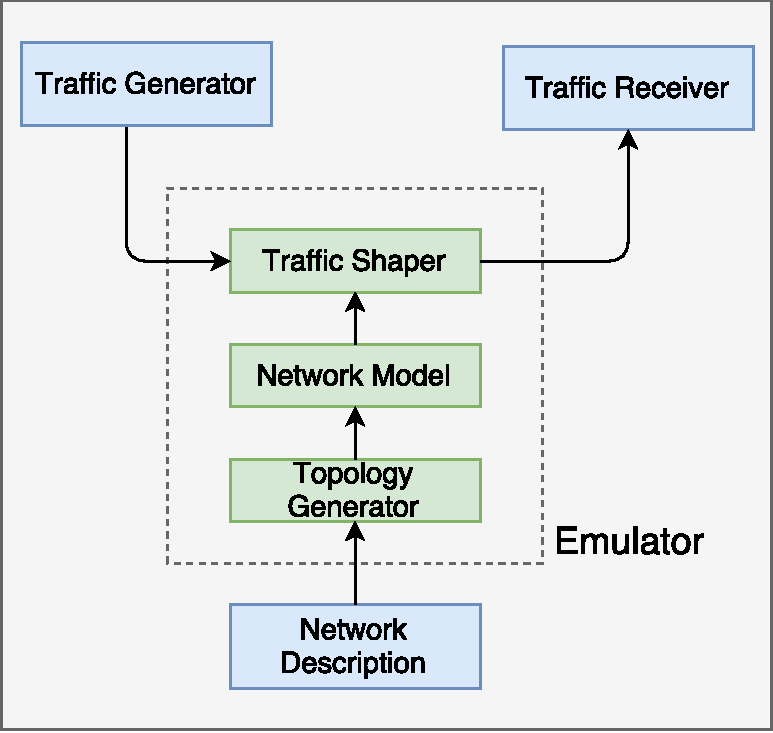
\includegraphics[width=0.5\textwidth]{emulator.pdf}}
	\caption{Basic structure of emulation}
	\label{fig:emulator}
\end{center}
\end{figure}

Definitions of the building blocks of emulation:
\begin{itemize}
	\item Application - here applications are the traffic generator or traffic receiver.
	\item Traffic Shaper - this is normally an operating system process which applies the physical properties (e.g., delay, bandwidth) of the target link in software. The traffic shaper must work in real time.
	\item Network Description - information about the nodes in the network, including position and relevant hardware information, along with the link description.
	\item Topology Generator - the topology generator translates the network description into a model of the network nodes and links.
	\item Network Model - a real-time description of the network nodes and links, including information about which links between which nodes are available and their characteristics (e.g., delay, bandwidth).
\end{itemize}

These are the basic elements of an emulator even though most emulators do not make a clear distinction between the different elements. This allows for a two-stage approach \cite{Perennou2005}, where the network description is converted to a network model in the first stage, and then the traffic shaper is applied on the network model in the second stage. This approach can be beneficial because the first stage does not have to be done in real time, so the computations can be more complex, allowing for more complicated phenomena to be considered. However, in the second stage, the application of the network model must still be done in real time.

\subsection{Real Network Testbeds}
Real network test beds use the actual implementation, along with the actual network links, to determine the performance of a network. This means that the test will be executed in real time, just as it would in real life scenario. Additionally, since the links are the actual physical links that would be used in real life, the results produced by a real network testbed would be an extremely accurate depiction of how the network would actually perform. The drawback to this approach is that it is very expensive and sometimes impossible to reconstruct. Every node in the scenario and the links connecting the nodes together has to be the same links that would be used in the actual network. For large mobile networks, this can be a very difficult task to faithfully represent it and the motion of the user device would have to be precisely reproduced. Even if the motion can be reproduced, the interference encountered by the nodes would have to be reproduced which might be difficult to attain \cite{Noble:1997:TMN:263109.263140}. Real network testbeds are also not very flexible since hardware changes must be made to create a different scenario. This forces the researcher to only consider a subset of the possible networks on which the application could be deployed.

\section{Software-Defined Network}\label{sec:sdn}
Software-Defined Networking (SDN) is an emerging concept that is dynamic, manageable, cost-effective, and adaptable, making it ideal for the high-bandwidth, dynamic nature of today's applications \cite{sdn-def}. Fundamentally, the SDN concept separates the network data plane, i.e., the network devices that forward traffic, from the control plane, i.e., the software logic that controls ultimately how traffic is forwarded through the network. The separation of the network's data plane and control plane allows the network operator to control network behavior from a single high-level control program. The main goal of SDN is to make the network more open and programmable. If an organization requires a specific type of network behavior, it can develop or install an application to do what it needs to do. These applications may be for networking functions, e.g., traffic engineering and security. There can also be applications for functionality that have not been thought of today and will be introduced in the future. This kind of flexibility would allow the network to evolve at the speed of the software. A desktop computer operating system model can be broken down to understand the SDN model. 

A desktop computer OS has three basic layers. First, there is the operating system itself that manages access of applications to underlying hardware. The OS also comes with core services to aid, i.e., responsible for managing system hardware on the lower level, e.g., CPU, storage, memory, and network interfaces. It can also be called the south of the OS instead of the lower level. Above the operating system, on the north side, are the applications. The ability to develop or add and remove applications makes the system a flexible one that can be customized to the costumers' specific needs whether gaming, design, engineering, and so on.

The SDN model also looks quite similar to the operating system model. In SDN, there is a network operating system or NOS instead of the operating system in the middle layer. This is also commonly called an SDN controller. The network operating system will typically have core services to aid in its job such as interfacing with network nodes and providing a programmable interface to the network applications. On the south side, instead of a hardware like a processor, storage, and memory, there are network forwarding devices that receive packets, take actions on those packets and update counters. The types of actions include simply dropping the packet, modifying packet headers, and sending packets out a single or multiple ports. The instructions on how to handle packets originate from the SDN controller. Like the desktop model on the top of the north side, there are applications, also called network applications, which similar to applications on top of a standard OS, can serve many purposes, but with SDN, are all network focused \cite{6994333}.

\begin{figure}[tb]
\begin{center}
	\resizebox{\textwidth}{!}
	{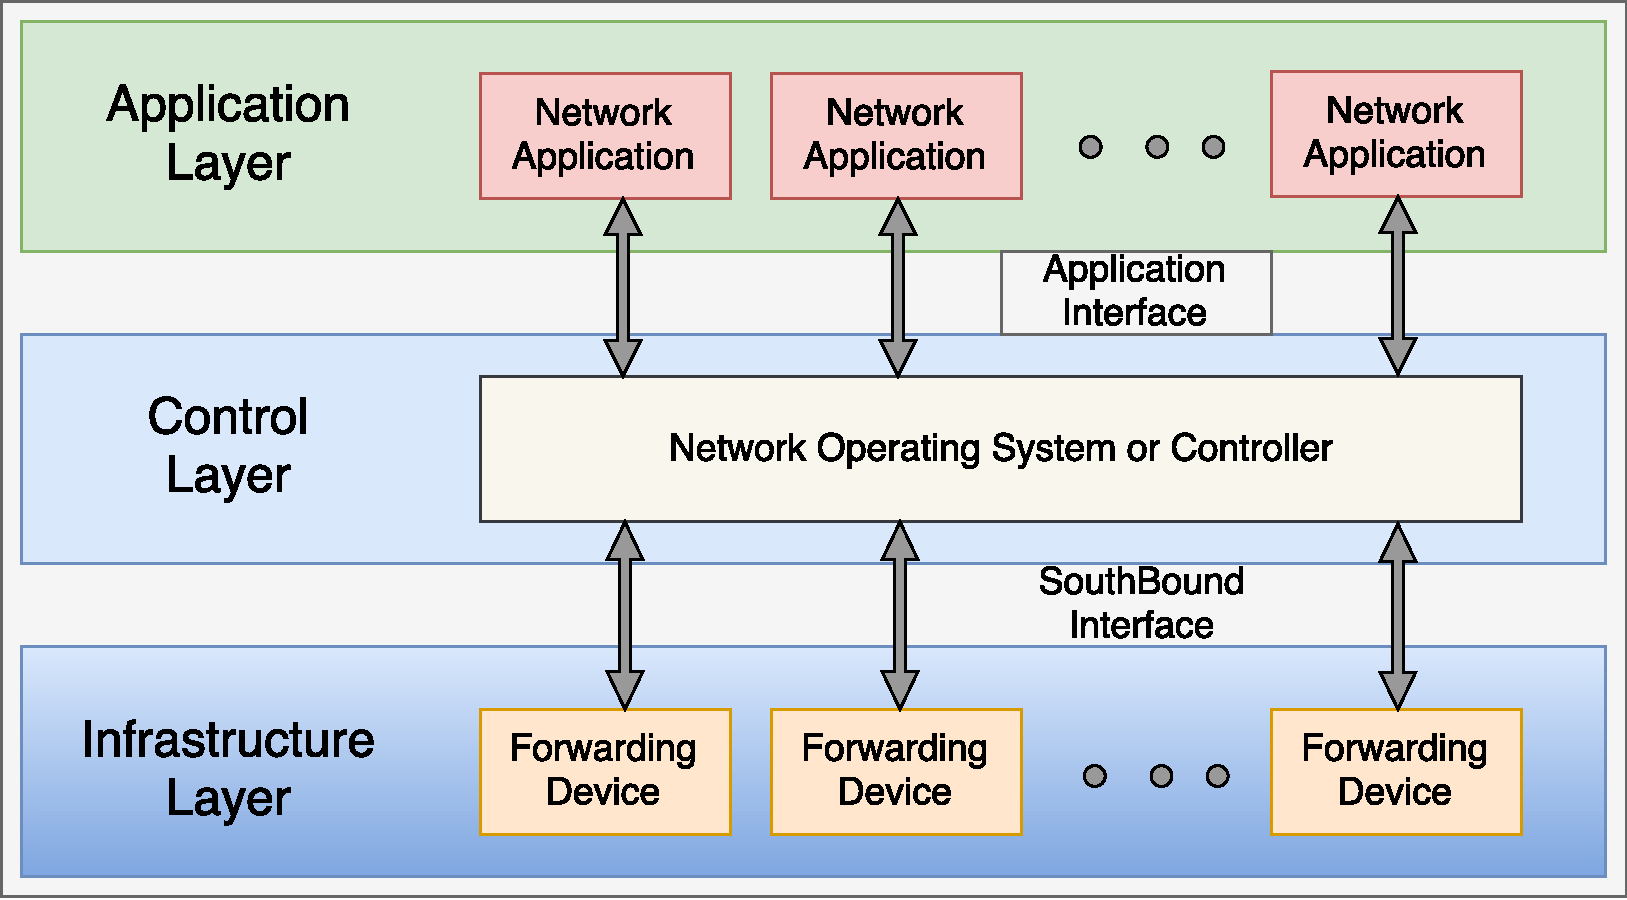
\includegraphics{sdn-architecture.pdf}}
	\caption{SDN architecture \cite{6994333} \cite{sdn-def}}
	\label{fig:sdnarch}
\end{center}
\end{figure}


Figure \ref{fig:sdnarch} provides an overview of the SDN model and its components, which are described in detail below.

\paragraph{Forwarding Devices:}
Forwarding devices, found at the lowest layer, can be conventional hardware switches as long as it support a programmable interface like OpenFlow (see Section \ref{sec:openflow}), or software switches like Open vSwitch (see Section \ref{sec:ovs}). Hardware switches are usually expected to support higher performance while software switches provide greater flexibility for new behaviors.

\paragraph{SouthBound Interface:}
The SDN controller needs a way to communicate with network forwarding devices. The information that needs to be communicated includes packet handling instructions, alerts of packet arrivals on network nodes, notifications of status changes like links going up or down, and statistics information like flow counters. All these happens over the southbound interface. The popular protocol for SDN on the southbound interface is OpenFlow for packet handling instructions. Complimentary to OpenFlow is the Open vSwitch Database Management protocol (OVSDB) \cite{ovsdbproto} which is a network management protocol used to manage network device configurations in Open vSwitch. It is also being adopted by some hardware-based switches.

\paragraph{Network Operating System:}
The network operating system is commonly referred to as an SDN controller. The controller typically runs with key core services, such as topology, inventory, and statistic services, and a host tracker. The topology service determines how forwarding devices are connected to one another and build what is known as a topology graph. For example, this might work by instructing switches to send Link Layer Discovery Protocol (LLDP) packets or other specialized packets and discovering where they arrived. An inventory service is used to track all SDN-enabled devices and record basic information about them, e.g., the version of OpenFlow and capabilities it support. A statistic service can be employed for reading counter information of floating devices like traffic counters on flows interfaces and flow tables. A host tracker discovers where IP address and MAC addresses of hosts are located in the network, typically by intercepting packets in the network or perhaps in coordination with the virtual machine (VM) platform.

\paragraph{Application Interface:}
The SDN controller provides application interfaces for network applications to hook into. It should be able to provide a simplified abstraction of the underlying network infrastructure often sufficient for the entire network fabric to be represented as a single large switch. For an application, there can be native plug-ins co-located with controllers and using a programming language-based application program interface (API) (e.g., Java API). There is a northbound interface as well, commonly a RESTfull interface which allows the use of standard HTTPS calls directed towards the controller to control network behavior and gather information collected by core services.

\paragraph{Network Application:}
Network applications can serve a wide range of disciplines. With SDN providing a programmable abstraction of the network, network applications can effectively be whatever an organization requires it to be in the context of controlling network behavior and implementing network policies.

\paragraph{}
As to how an SDN network works differently compared to today's conventional networks, below are some important concepts \cite{sdn-def}.

\paragraph{Fault tolerance and scalability:}
Commonly, an SDN controller is referred to as being logically centralized. It is important to understand how this is different from being physically centralized. In a production network, no one would depend on a single physical SDN controller. This would lead to a single point of failure for the entire network, and additionally, there could be scaling limitations. There are different ways to ensure that SDN network is both highly available and scalable. One is clustering and teaming, which is not new in areas like database servers. The idea is to have a cluster of systems that can load balanced workload and provide high availability since one or more systems can break down, ensuring there are still active functional systems. This also provides scalability as multiple systems can handle requests. 

Additionally, the network can be separated into different regions with each region's traffic handled by a regional SDN controller. Different regions can then communicate information between one another as needed using an east-west protocol. SDN controllers also might be designed in a hierarchy. There may be high-level controllers with high levels of abstraction and lower level controllers underneath closer to the network forwarding devices \cite{6994333}.

\paragraph{Directly programmable:} This gives the flexibility to network administrators who directly program network control because it is separated from forwarding devices \cite{sdn-def}.

\paragraph{Agile:} Abstraction of the control from forwarding devices allows administrators to dynamically adjust network-wide traffic flow to achieve changing needs of the environment \cite{sdn-def}.

\paragraph{Programmatically configured:}
SDN allows network managers to write dynamic, automated SDN programs to configure, manage, secure, and optimize network resources very quickly \cite{sdn-def}.

\paragraph{Open standards-based and vendor-neutral:} SDN is implemented through open standards-based which simplifies network design and operation. The control instructions are provided by SDN controllers rather than multiple, vendor-specific devices and protocols \cite{sdn-def}.

\paragraph{Conventional Network Devices}
\paragraph{}
In conventional networks, nodes have a data plane and a control plane both contained within a single physical system. The function of the data plane is to handle packets and line rate in hardware based on information stored in tables like the FIB, LFIB and MAC tables. Execution instructions in the data plane originated in the control plane. The control plane is sometimes referred to as the network nodes brain. The network node uses the control plane to communicate with other nodes in the network. They usually run distributed protocols like BGP, MPLS, and OSPF. Thus, the control plane handles the complexity and it is where network policies are enforced. The control plane determines how individual packets should be handled and pushes this information down to the fast path in the hardware-based data plane. 

Different from the SDN ecosystem discussed earlier, conventional network nodes are, first, proprietary locked boxes. Second, the control plane is chained in the data plane and both are coupled together in a single network node. There is no direct access to the behavior of the data plane to implement network policies so that network operators have to think in terms of what is already available in the control plane or what features or options the device include. Operators most often configure the device through a command-line interface. If a new kind of network behavior is required, options can be limited. 

Another disadvantage of a conventional network compared to an SDN network is that each network node has to be configured individually, so the network operator needs to deal with multiple points of configuration. In a data center, for example, there could be tens or hundreds of nodes to reconfigure to implement new policies. Each of these nodes has its own control plane and all these control planes must communicate using distributed protocols. Therefore, this conventional network paradigm is typically complex and can lead to configuration error as cited earlier \cite{6994333}. 

By contrast with SDN, conventional networks have a lengthy vendor equipment product life cycles. It does not have any specific standard and the lack of open interfaces limit the ability of network operators to adapt the network to their individual environment's requirements \cite{sdn-def}. However, it is important to note that significant complexity may be present in the architecture of the SDN controller itself to accomplish all of its benefits.

\subsection{OpenFlow}\label{sec:openflow}
As previously mentioned, OpenFlow is the standard communications interface defined between the control and forwarding layers of an SDN architecture \cite{openflow}. OpenFlow allows direct access to SDN-enabled devices, such as switches and routers, both physical and virtual. In the SDN architecture (see Figure \ref{fig:sdnarch}), business requirements come into play in the control layer. A control layer software figures out how to translate these requirements into commands to the switches and instructs how to route traffic. The OpenFlow protocol conveys that information to the switches and the switches process the traffic as it comes through. Thus, OpenFlow is a standardized protocol for interaction and manipulation of the forwarding plane or network devices such as switches and routers.

\paragraph{Switch Components}
\paragraph{}
Logically, an OpenFlow switch has one or more flow tables and a group table, which are responsible for packet lookups and packet forwarding. It has also one or more OpenFlow channels to connect to the controller (see Figure \ref{fig:ofscomp}). Both the switch and controller can communicate through such channel and the controller manages the switch using the OpenFlow switch protocol. The controller can add, update, and delete flow entries in flow tables using the OpenFlow switch protocol. The update can happen reactively, i.e., in response to packets, and proactively. Each flow table in the switch has a set of flow entries and each flow entry has a match of fields, counters, and a set of instructions to apply to the matching packets. The group table comprises group entries and each group entry has a list of action buckets with specific semantics based on group type. The actions from one or more action buckets are applied to packets before sending it to the group \cite{openflowspecification13}.

\begin{figure}[H]
\begin{center}
	{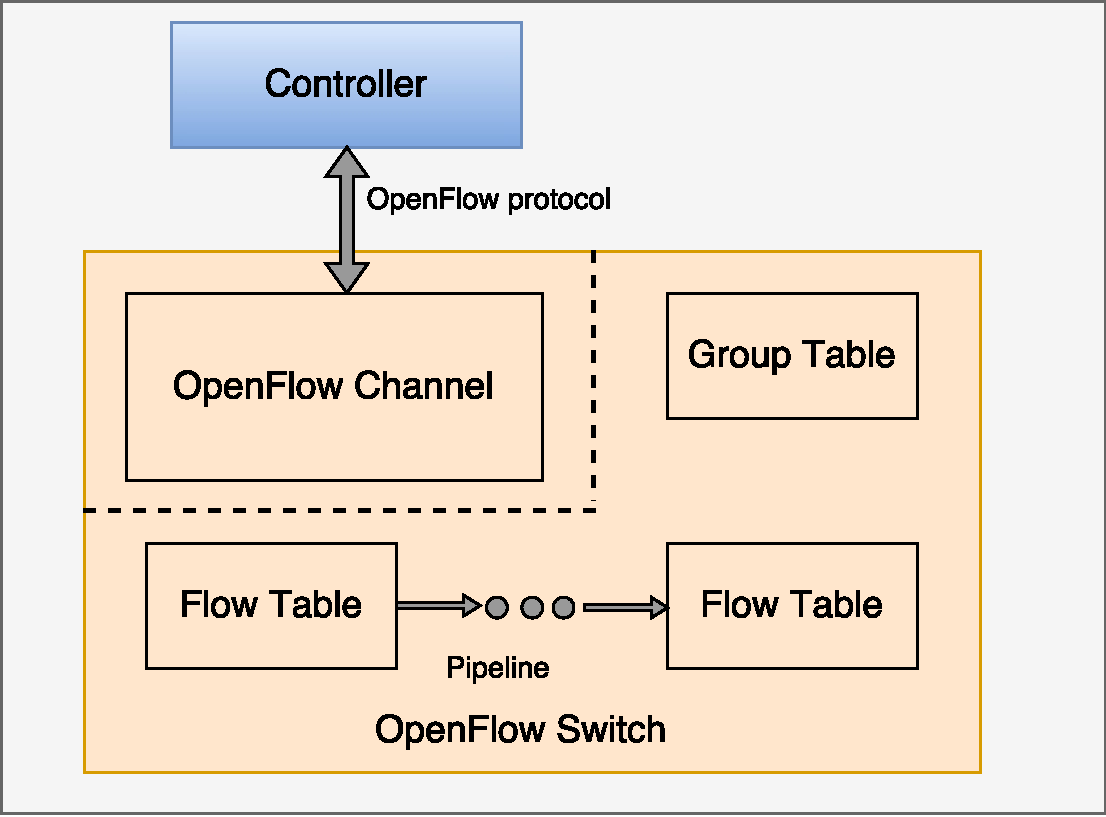
\includegraphics[width=0.75\textwidth]{openflowswitchcomponent.pdf}}
	\caption{Components of an OpenFlow switch \cite{openflowspecification13}.}
	\label{fig:ofscomp}
\end{center}
\end{figure}

\paragraph{Packet Processing}
\paragraph{}
The OpenFlow table entry consists of three fundamental parts, a match field, a counter, and an instruction (see Figure \ref{fig:oftcomp}). The match field dictates what to match in an incoming packet.

\begin{figure}[H]
\begin{center}
	\resizebox{\textwidth}{!}
	{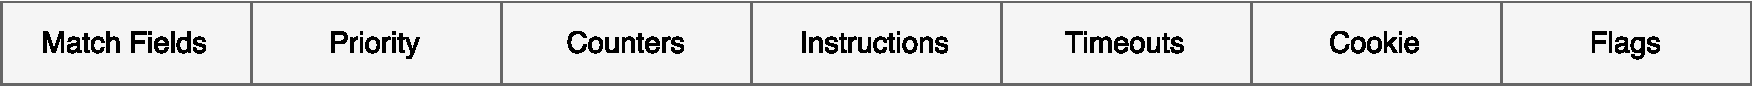
\includegraphics{openflowtablecomponent.pdf}}
	\caption{Components of a flow entry in a flow table \cite{openflowspecification13}.}
	\label{fig:oftcomp}
\end{center}
\end{figure}

On packet arrival, switch matches the header of the packet with the flow entries in a table. If any entry matches, it updates the counters of the entry and performs the specified action. Matching starts at the first flow table and may continue to additional flow tables of the pipeline (see Figure \ref{fig:ofscomp}). The match can happen in a priority order. If no match is found in a flow table for an incoming packet, the outcome depends on the configuration of the table-miss flow entry. For example, the packet may be forwarded to the controller over an OpenFlow channel, dropped, or may continue to the next flow table (see Figure \ref{fig:ofpacketflow}) \cite{openflowspecification13}. Different counters are maintained in OpenFlow, which count the number of packets and bytes at various specific points of the pipeline. There can be a counter for each flow table, flow entry, port, queue, group, group bucket, meter and meter band.

\begin{figure}[H]
\begin{center}
	{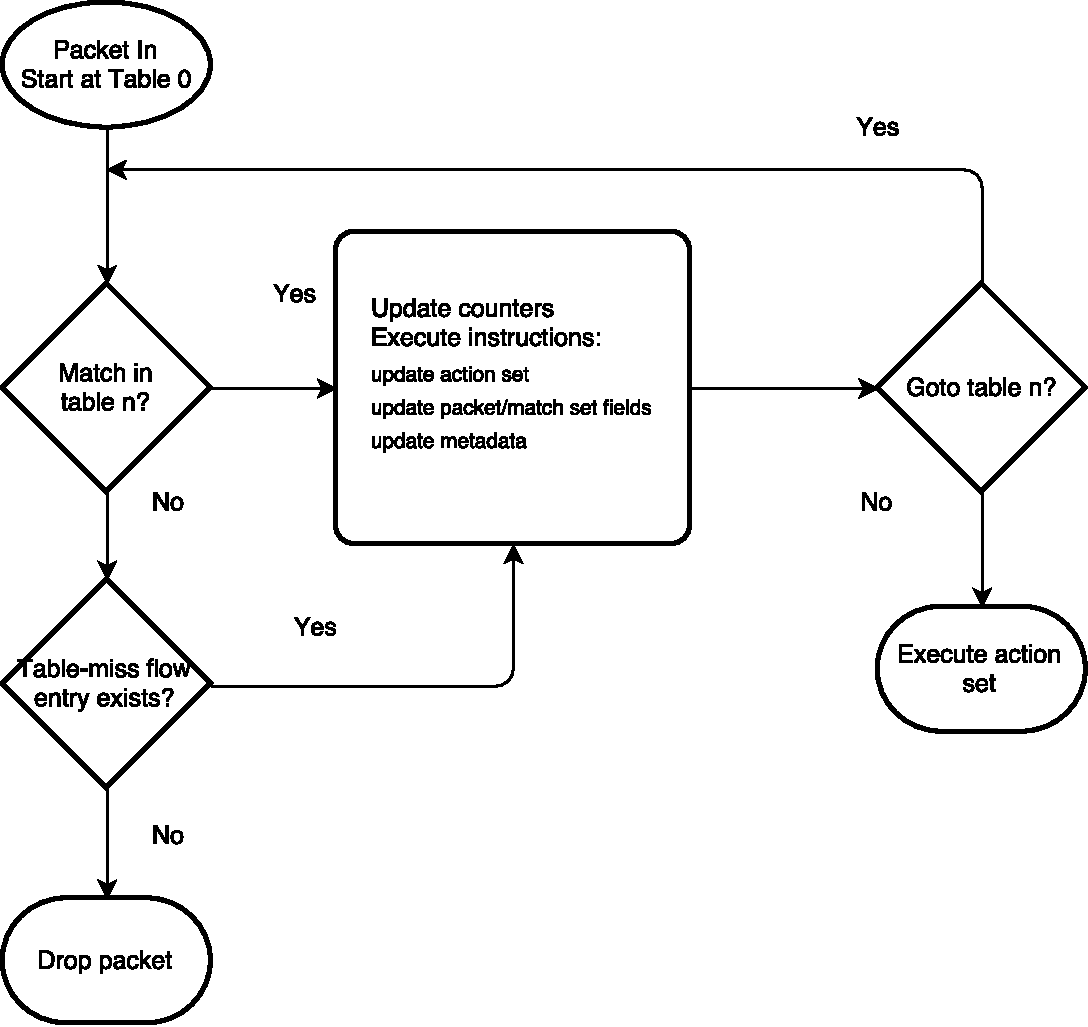
\includegraphics[width=0.75\textwidth]{openflowpacketflowchart.pdf}}
	\caption{Flowchart detailing packet flow through an OpenFlow switch \cite{openflowspecification13}.}
	\label{fig:ofpacketflow}
\end{center}
\end{figure}

Each flow entry consists of an instruction to execute an action on the packet or modify pipeline processing. The valid action could be packet forwarding, packet modification, and group table processing. Pipeline processing passes information in the form of metadata to allow further processing of the packet and sent to the next table. Pipeline processing does not continue when the instruction set associated with a matching flow entry does not mention the next table, which signifies that the packet was already modified and forwarded. Actions associated with flow entries may also direct packets to a group, which means additional processing has to be done. Groups usually represent a set of actions for flooding, as well as more complex forwarding semantics such as multi-path, fast reroute, and link aggregation \cite{openflowspecification13}.

\paragraph{OpenFlow Channel}\label{par:ofc}
\paragraph{}
The OpenFlow channel is the interface that connects each OpenFlow logical switch to an SDN OpenFlow controller; a controller may have connection setup with multiple switches. On the other hand, a switch may have connections with multiple controllers. Having multiple controllers improves reliability as the switch can continue to operate in OpenFlow mode if one controller or the connection fails. Normally, the switch initiates the connection setup with the controller using the host and port configured in the switch. Once the connection channel is set up, communication can happen in both ways, i.e., controller to switch and switch to the controller. The OpenFlow protocol supports three message types: controller-to-switch, asynchronous, and symmetric, each with multiple sub-types \cite{openflowspecification13}. Controller-to-switch messages are initiated by the controller and may or may not require a response from the switch. Asynchronous messages are sent without a controller soliciting them from a switch. Symmetric messages are sent without solicitation, in either direction so any side can initiate a conversation anytime as needed.

\subsection{Open vSwitch}\label{sec:ovs}
Open vSwitch (OVS) is an OpenFlow-capable multi-layer (it can operate at layers 2, 3 and 4) virtual switch. It is typically used with hypervisors to interconnect virtual machines within a host and virtual machines between different hosts across networks. It is also used in some dedicated switching hardware and is an important component in an SDN solution. It works on a number of different platforms including Linux and FreeBSD. It can be configured remotely as well as locally on the box.

\begin{figure}[H]
\begin{center}
	{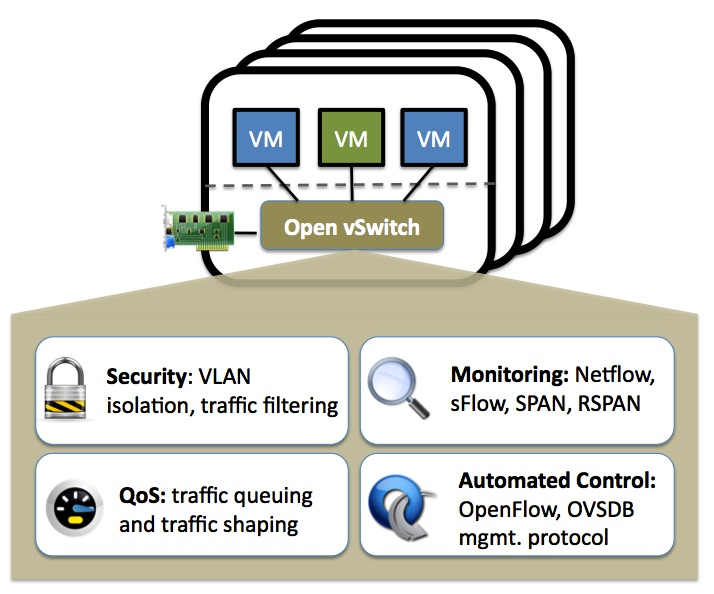
\includegraphics[width=0.75\textwidth]{ovs-overview.png}}
	\caption{Open vSwitch overview \cite{ovswhatis}.}
	\label{fig:ovsoverview}
\end{center}
\end{figure}

Open vSwitch supports many conventional switch features such as Standard 802.1Q virtual LAN (VLAN) model with trunk and access ports, Network interface controller (NIC) port bonding, Link Aggregation Control Protocol (LACP) and various tunnelling method like Geneve, Generic Routing Encapsulation (GRE), Virtual Extensible LAN (VXLAN), Stateless Transport Tunneling (STT), and Locator/ID Separation Protocol (LISP). It also supports many important features like NetFlow, sFlow, mirroring for increased visibility, QoS (Quality of Service) configuration, and policing. It supports OpenFlow 1.0 plus its numerous extensions. OVS can be run in both kernel and user space. It is also included in Linux kernel \cite{ovswhatis}.

\subsubsection{Open vSwitch Components}

\begin{figure}[H]
\begin{center}
	\resizebox{\textwidth}{!}
	{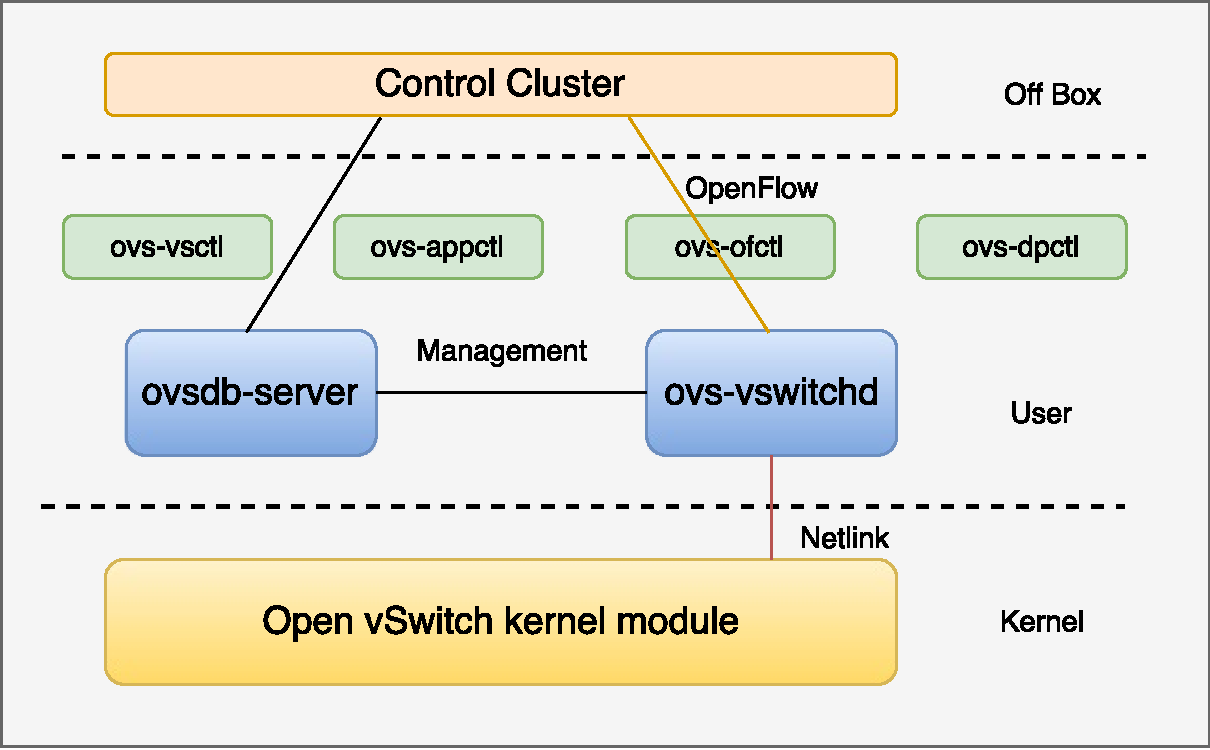
\includegraphics{ovs-components.pdf}}
	\caption{Open vSwitch components.}
	\label{fig:ovscomponent}
\end{center}
\end{figure}

OVS consists of three main components (see Figure \ref{fig:ovscomponent}), ovsdb-server, ovs-vswitchd, and the OVS kernel module. In the upper part of the figure is the control cluster that could be an OpenFlow controller e.g., Ryu, Floodlight, NOX, etc. Ovsdb-server is the component that has the configuration database which is state-full, i.e., information will survive a reboot. It has configuration settings for things like bridges and interfaces. A daemon ovs-vswitchd is the core part of Open vSwitch; it implements the switch and does all of the handlings of flow setups. Open vSwitch kernel module is, in actuality, a cache of recently seen traffic. OVS has different communication protocols (e.g., OpenFlow, Netlink, Management) for improved performance. Different components use them to talk with each other \cite{Pfaff:2015:DIO:2789770.2789779}. The following describes all OVS components in detail:

\paragraph{OVS kernel module:}
The OVS kernel module is mainly responsible for switching and tunnelling and it is a fast cache of non-overlapping flows. It is designed to be fast and simple, it does not know anything about OpenFlow; it simply implements the tunnels.

\paragraph{Ovs-vswitchd:}
Ovs-vswitchd is the core component of the system. It speaks up to the controllers with OpenFlow, to the database server over a management protocol, and it communicates with the kernel module over Netlink on Linux. The command tools that is used to deal with OVS are ovs-vsctl and ovs-appctl.

\paragraph{Ovsdb-server:}
Ovsdb-server holds all the switch level configuration, information about creating bridges, attaches interfaces to bridges, creates tunnels attach to bridges, etc. It also has ovsdb and the OpenFlow controller address. Ovsdb-server stores the configuration eternally and has all the properties of a database. One area of implementation is that it is log-based, i.e., rather than just storing the state of the database, it also contains the changes that have happened, making it very useful for debugging. Ovsdb-server uses a JSON-RPC \cite{jsonrpc}-based protocol for communication.

\paragraph{Ovs-vsctl:}
Ovs-vsctl configures ovs-vswitchd, but it is basically a high-level interface for the database. It can be used for a lot of utilities in OVS, such as configuring the system, looking at the state of the system, among others.

\paragraph{Ovs-ofctl:}
Ovs-ofctl is a utility for querying and controlling OpenFlow switches and controllers. It is used for configuring OVS and uses OpenFlow to the switch, similar to an ovs-vsctl communicating to the ovsdb-server. Typically, ovs-ofctl uses the OpenFlow protocol to the switch over a local socket. Ovs-ofctl can perform operations like dumping the flow table, adding a flow, or deleting flows.

\paragraph{Ovs-dpctl:}
Ovs-dpctl is a tool for configuring the switch kernel module. It can be used to configure the datapath, look at the flow table that has pushed down into the datapath, and dump flows.

\paragraph{Ovs-appctl:}
ovs-appctl is a utility that sends commands to running Open vSwitch daemons. It is used to make changes to or to query the runtime status of the switch.

\section{Flow processing-aware Control Application Placement Framework}\label{sec:fcpf}
Increasing demands of high-quality network service result in different innovative network communication techniques such as CoMP and VNF. These techniques impose more data flow in the network and have several constraints, such as low level of latency and high data rate along with additional processing requirements in the network. Considering all these constraints, accommodating all these techniques requires efficient and flexible management of the underlying backhaul network. 

Recent works \cite{7343600} \cite{aurouxew2017} assume that these techniques can be realized by Control Applications (CAs), acting as functions in the sense of Network Function Virtualization (NFV) \cite{nfv-arch}. Placing these CAs in a suitable location is a challenging task, especially since the traffic load of a mobile network changes very quickly and the performance of a static placement will worsen over time. In modern dense and crowded networks, many data flows appear and expire every second. To reduce reconfiguration overhead, any reassignment should take into account the existing placement. This problem is addressed by a flexible FCAP framework (FlexFCAPF) solution approach. FlexFCAPF places CAs in a suitable location in the network and eventually flexibly reassigns those based on the previous CAs placement in reaction to changes in network load levels.

\begin{figure}[H]
\begin{center}
	\resizebox{\textwidth}{!}
	{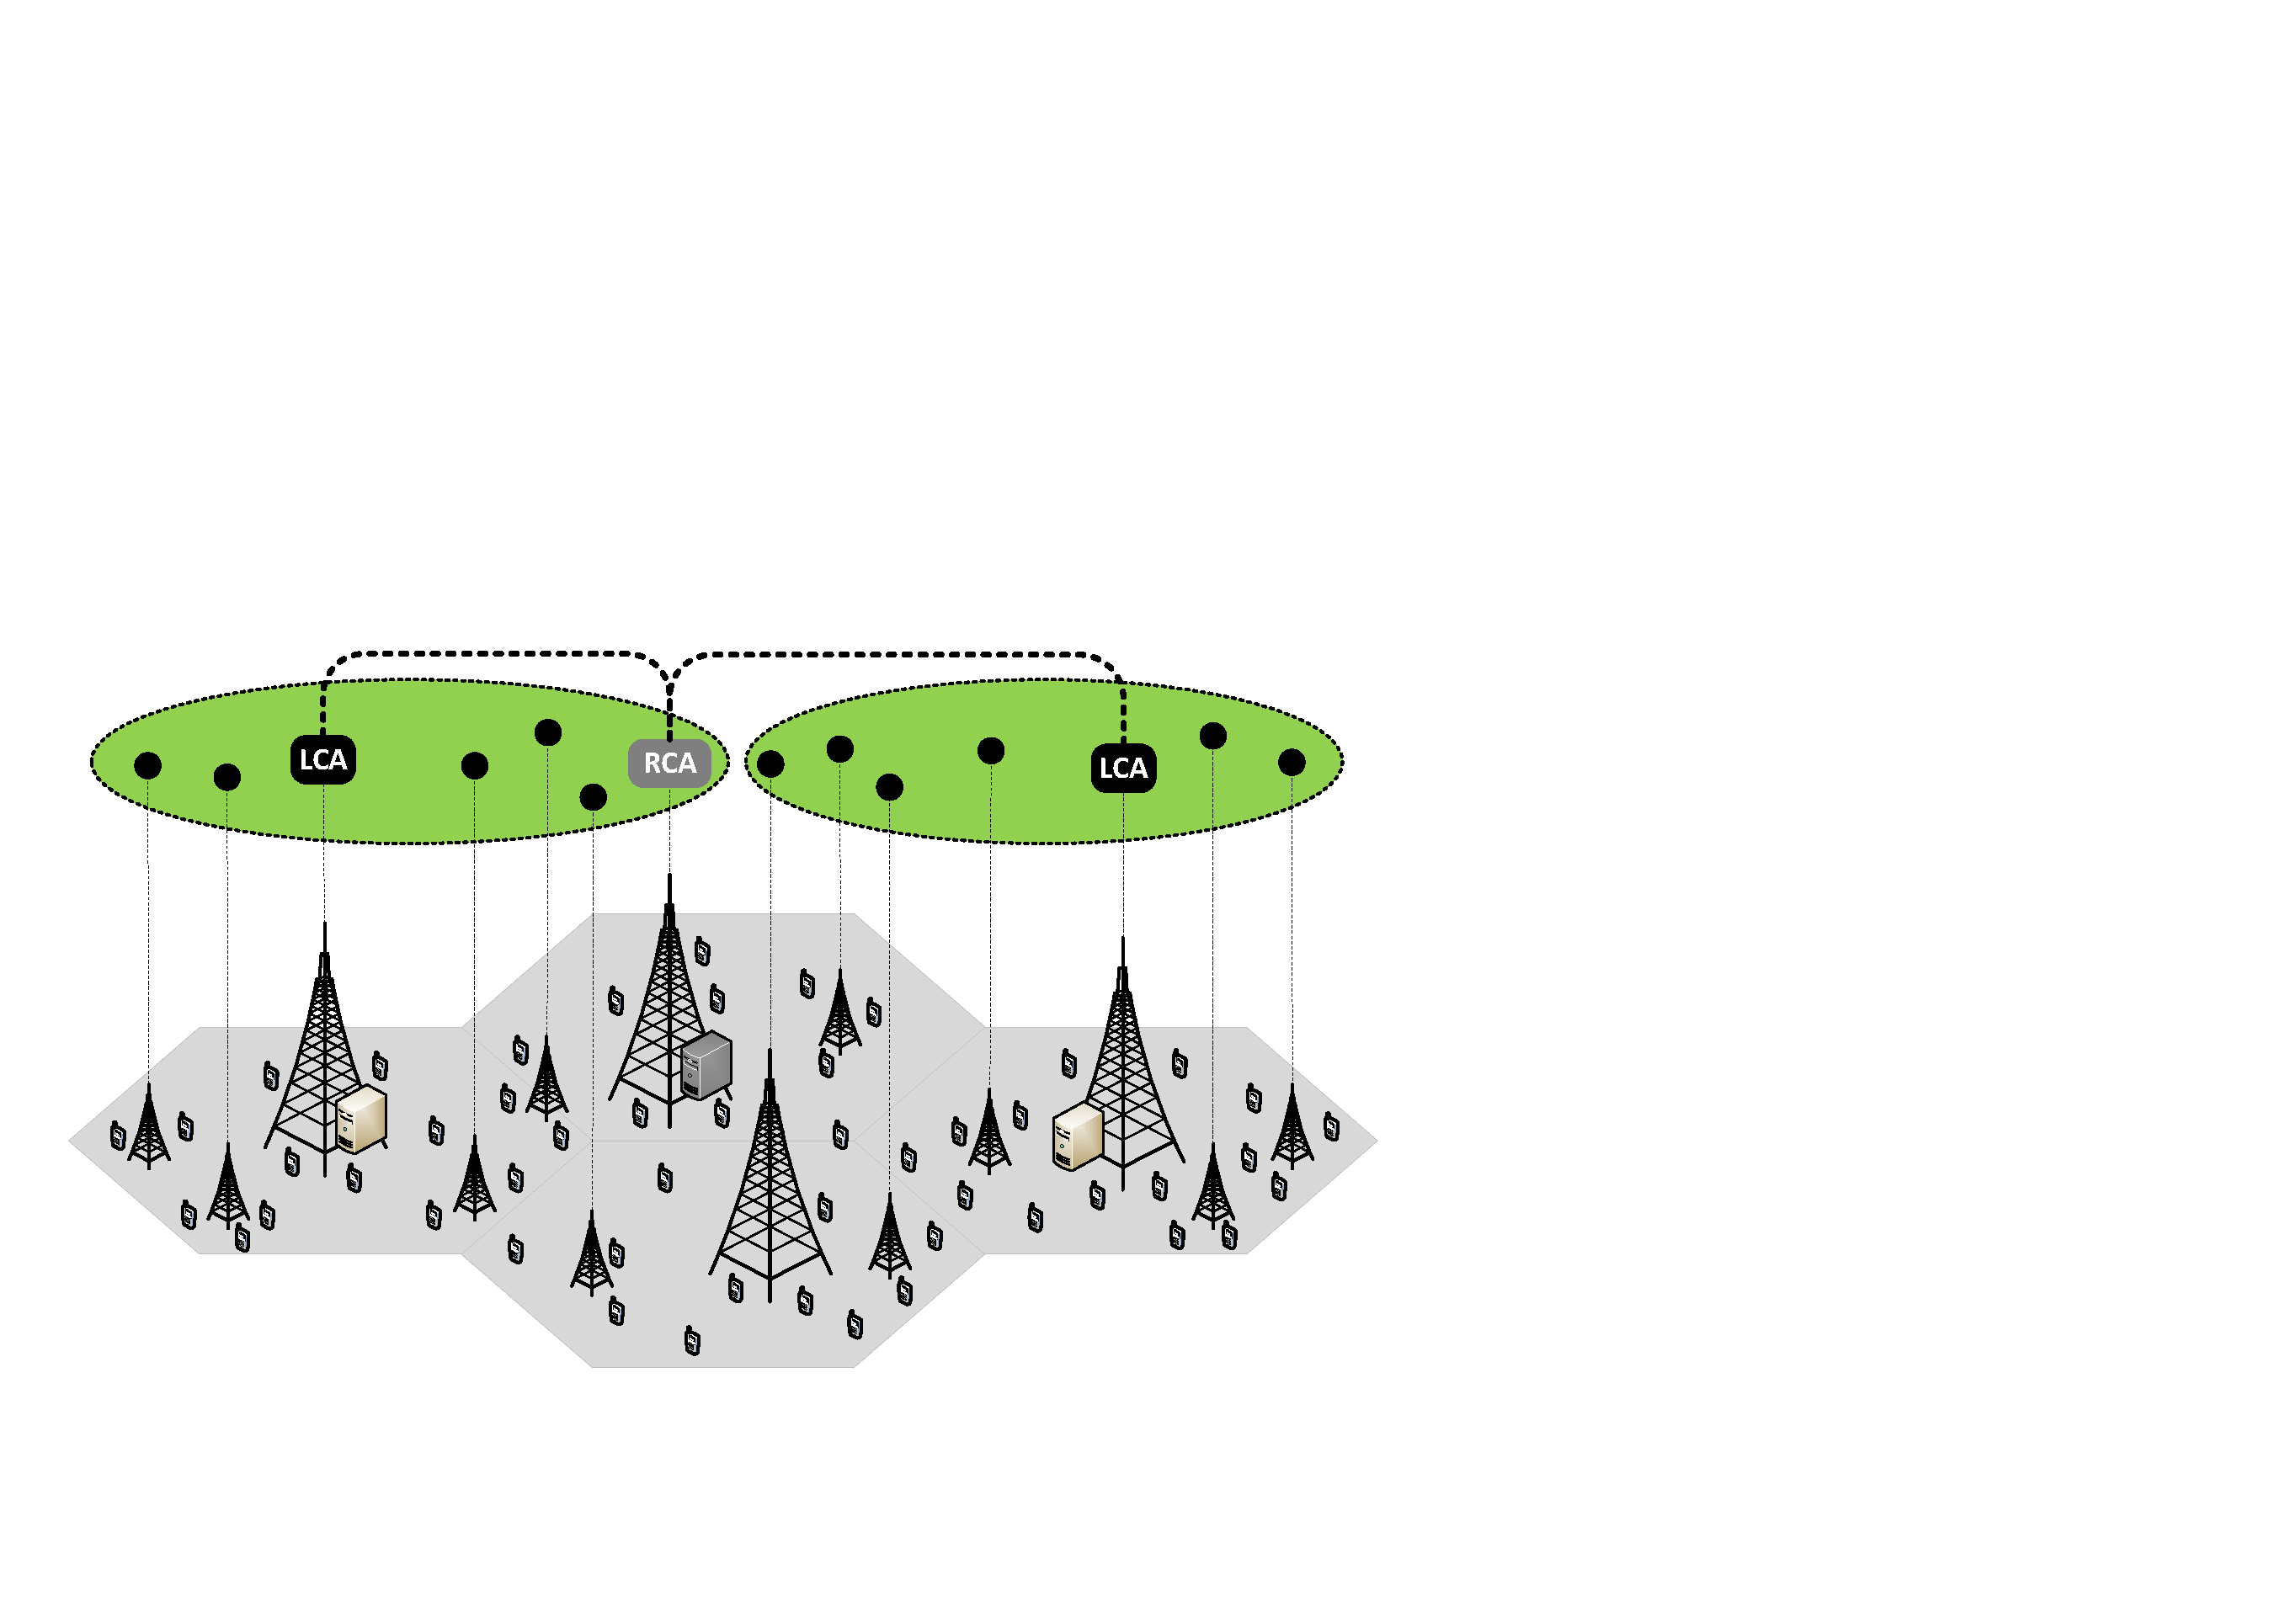
\includegraphics{fcapp-scenario.pdf}}
	\caption{Typical FCAPP framework scenario \cite{aurouxew2017}.}
	\label{fig:fcpfscenario}
\end{center}
\end{figure}

FlexFCAPF architecture consists of a two-tier hierarchical structure of CAs. They are Local Control Applications (LCAs) and Regional Control Applications (RCAs). The LCAs operate locally with limited scope and can execute faster, typically work as a data processing application. The RCAs operate globally with a bigger scope, thus, it can have the myopic view of the local CAs. They typically work as a coordinator of the LCAs. This two-tier hierarchical architecture allows to have a better aggregation of network information, resulting to reduced signaling overhead. Both LCAs and RCAs are seen as CAs acting as functions in the sense of NFV. They can be instantiated on a network equipment that is fulfilling the necessary hardware requirements, i.e., sufficient memory and processing capacity. The high-level coordination of RCAs can be omitted if it is desired. A one-tier hierarchy can be expressed by simply setting all RCA requirements to zero. To illustrate the architecture, Figure \ref{fig:fcpfscenario} shows a typical FlexFCAPF scenario and a possible control structure with one RCA and two LCAs.

FlexFCAPF problem statement and the solution approach are based on the description in \cite{7343600} \cite{aurouxew2017}.
\subsection{FlexFCAPF Problem Statement}\label{sec:ffps}
The job of FlexFCAPF is to place CAs appropriately into a given network, along with satisfying the DFGs available in the network. While doing this, FlexFCAPF considers some constraints such as data processing and latency constraints, along with the network constraints usually associated with network control. FlexFCAPF take an input backhaul network (e.g., Wireless Access Network) as a graph $G = ( V, E )$ with nodes $V$, e.g., switches, and undirected edges $E$, which is representing the links of the network. All nodes in the network may not have the capability of hosting a CA, i.e., fulfill the hardware requirements of becoming a CA, therefore FlexFCPF denotes that capable node by $C \subseteq V$. The processing power of the node is denoted by $p_{node} ( c )$ FLOPS where $c \in C$. The link between two node is denoted by $( u, v ) \in E$ and a link has a maximum data rate of $b_{cap} ( u, v )$ bit/s and a latency of $l_{cap} ( u , v )$ seconds. FlexFCAPF considers the latency of a link independent of the network load and ignores possible queuing delays.

A solution of the given network is achieved by creating a complete control structure, i.e., each node of the network $v \in V$ is controlled by at least one LCA (a node can be controlled by more than one LCA if needed for optimal network performance) and each LCA is required to be coordinated by exactly one RCA. An LCA needs a processing capacity of $p_{LCA}$ FLOPS per controlled node for becoming the LCA of a node while an RCA needs a processing capacity $p_{RCA}$FLOPS per coordinated LCA for becoming the RCA of an LCA. Also, a path must exist between a node and its LCA and a round trip latency cannot be more than $l_{LCA}$ seconds and should provide a minimum data rate of $b_{LCA}$ bit/s. The routing path between a node and its LCA needs to have at most a round trip latency of $l_{LCA}$ seconds and a minimum data rate of $b_{LCA}$ bit/s. Similarly, the path between an LCA to its RCA need to have a round trip latency $l_{RCA}$ seconds and a minimum data rate of $b_{RCA}$ bit/s.

Furthermore, FlexFCAPF denotes the Data Flow Groups (DFGs) on the network as a set $F$. Each DFG contains one or multiple (to represent scenarios like CoMP) data flows, and enters the backhaul network through a node from $V$. The data flows of one DFG may originate from different nodes in the network but all of them has to be processed by the same LCA jointly. The connection matrix $W \in \{ 0, 1 \}^{| F | \times | C |}$ is used to represent the relationship between DFG and the set of network nodes. The processing LCA of a DFG should provide a processing power of $p_{flow} ( x )$ FLOPS for processing every data flow from each DFG $x \in F$. The routing path between the LCA and the nodes through which the DFG is entered in the network need to provide a maximum round trip latency $l_{flow} ( x )$ seconds and a data rate of $b_{flow} ( x )$ bit/s. For simplicity, FlexFCAPF considers the full round trip for all DFGs, so that FlexFCAPF solution fully incorporates request and response traffic.

A DFG $x \in F$ is said to be satisfied by an LCA $c \in C$ if and only if
\begin{enumerate}
	\item $c$ controls all nodes $v$ with $W_{x,v} = 1$ and
	\item the routing paths from all nodes $v$ with $W_{x,v} = 1$ to $c$ have sufficient resources to provide a data rate of $b_{flow} ( x )$ and a round trip latency $l_{flow} ( x )$.
\end{enumerate}

It is important to remember, that the round trip latency in the network is not only the travel time of the data flow. It also includes the time necessary for processing the data flow $x$ at $c$. Therefore, to enable a round trip latency $l_{flow} ( x )$, a sufficient amount of processing capacity from $c$ has to be allocated for $x$ to handle $p_{flow} ( x )$ FLOPS and the link delays in time.

\subsection{FlexFCAPF Solution Approach}
The objectives of FlexFCAPF are as follows, listed in descending order of importance:
\begin{enumerate}
	\item Create a valid solution, i.e. a complete control structure,
	\item Maximize the number of satisfied DFGs, and
	\item Minimize the number of used CAs.
\end{enumerate}

The main objective of FlexFCAPF model is to provide a fully functional valid network solution, i.e., a complete control structure with the maximum number of DFGs are satisfied by an LCA. However, DFGs being satisfied at any point of time may not be possible at all events. This is because the network might have many DFGs entered at some point in time but it does not have enough resources to satisfy all. In such a situation, FlexFCAPF might result in an incomplete control structure, i.e., not all nodes are correctly controlled, which is why creating a complete control structure is more important for the network than a couple of yet unprocessed DFGs. Saving network resource is an important objective from an operator's point of view and minimizing the number of used CAs is preferred in saving such costs. On the other hand, dropping DFGs would reduce Quality of Service (QoS) and will eventually frustrate customers. Therefore, minimizing the number of used CAs is given less importance than DFG satisfaction and feasible only if it does not affect the network's performance.

My considered version of FCAPP assumes that the schedule for data processing at an LCA is First Come First Serve (FCFS) scheduling. This means that the LCA will allocate the requested processing power by any DFG and that particular DFG will hold that amount of processing power until it finishes the job. The LCA will also allocate the amount of processing power required by all its controlled nodes. FlexFCAPF determines the required routing paths to guarantee that no constraint for network control and DFG processing is violated, and verifies that all conditions are satisfied at any point in time. The implementation of the algorithm will be elaborated in section \ref{sec:algoadap}.

\section{Tools and Technology}\label{sec:tools}
The different approaches of testing computer network application was described in section \ref{sec:nta}. Simulation and emulation provide a solid base to determine the pros and cons of a netwrok application. However, emulation is more realistic than simulation since it must be carried out in real time and could provide a way to some real devices running real operating systems to interact with some simulated devices \cite{6588659}. Moreover, recent works \cite{7343600} already evaluated FlexFCAPF model by simulation. In this study, FlexFCAPF will be evaluated in the emulation environment, thus selecting appropriate tools and technologies for building an emulation testbed is necessary. The following paragraph describes the basis for selecting those tools and technologies. A brief description of their features and functionalities is also given in the later section.

First, a platform had to be chosen where FlexFCAPF can be adapted easily. There are not many SDN platforms available for use, and for these Mininet \cite{Lantz:2010:NLR:1868447.1868466}, MaxiNet \cite{6857078}, EstiNet \cite{6588659}, NS-3 \cite{ns-3}, DOT \cite{6838241} and OFnet \cite{ofnet} were compared. NS-3 is an open source platform and available free of use. It has an OpenFlow simulation model and it offers a realistic OpenFlow environment. However, it does not support real OpenFlow controllers, so they developed their own controller but it does not support latest OpenFlow protocol \cite{al2014survey}. 

EstiNet is one of the best emulators which provide correct, trustworthy performance result and high scalability \cite{6588659}. EstiNet provides distributed emulation across multiple machines with an added feature of time dilation. However, there are not many details available about the technique used by EstiNet and how to use it as it is a closed-source proprietary platform. 

DOT is a low cost and scalable network emulator. In the paper \cite{6838241}, DOT is claimed to emulate large-scale SDN deployment, overcoming the scalable limitation of Mininet. The paper also suggested that DOT provides guaranteed CPU time, bandwidth, and network latency for the emulated components (i.e., switches, hosts, and links). It scales with the network size and traffic volume, has a built-in central system for configuring and monitoring the emulated components, and makes it possible to run any customizable controller. DOT looks like a promising option for the testbed setup since it matches most of my testbed requirements, except for data processing capability. It was not specified, however, how scalable the environment is and no practical example to use DOT was given, neither any reliable implementation example can be found. 

OFnet is another easy-to-use platform to setup SDN network emulation and it comes with a friendly Apache v2 license. It provides some interesting features such as visual debugging of control plane transactions and traffic generation on emulated network. Developers claim these features enable the user in characterizing the performance of an SDN controller. The traffic generation feature of OFnet is interesting for my testbed but it does not provide much flexibility such as in generating controlled traffic. Similar to DOT, OFnet also lacks practical implementation and is not usually used in testing. 

Mininet is one of the most popular SDN platform used by many SDN researchers because of its simplicity, availability, and flexibility. It also fully supports OpenFlow architecture \cite{Lantz:2010:NLR:1868447.1868466}. However, Mininet is not scalable and can not be deployed over multiple machines. This limitation is resolved in MaxiNet. MaxiNet is basically an extended platform based on Mininet which can be deployed over multiple servers connected via a network. Since MaxiNet supports the existing Mininet API with minimal alteration and Mininet has been used in many SDN testbed emulations projects, I decided to use Mininet for small-scale testing and MaxiNet for large-scale testing.

One important aspect of FlexFCAPF model is that it generates the flow path of the traffic flow it satisfies as part of the solution. Therefore, an OpenFlow controller is needed which can be used to configure the generated flow path in the network dynamically. The OpenFlow controller should be easily customizable, compatible to Mininet/MaxiNet, component-based. For this purpose, NOX \cite{nox}, POX\cite{pox}, Floodlight \cite{floodlight}, OpenDaylight \cite{opendaylight} and Ryu \cite{ryu} were compared. 

NOX controller is one of the first controllers of OpenFlow written in C++ language. Its first version provides an API for Python scripts, but the last version of NOX has dropped the API support and kept only C++. NOX provides a high-level, programmable interface upon forwarding devices and applications. It is designed to support both small networks of a few hosts and large enterprise networks of hundreds of switches and hosts. NOX's core has features of fast, asynchronous I/O, topology discovery, host tracking possibility, and learning switch feature. Researchers discovered that NOX does not support the iperf command properly which determines the bandwidth utilization \cite{al2014survey} and is an important requirement for this study's testbed since iperf will be used to generate controlled traffic. NOX's documentation support is very poor and its mailing-lists are almost abandoned. 

POX is the younger sibling of NOX; the main difference is that it is developed in Python instead of C++. POX uses Python API to support network virtualization, SDN debugging, and different applications such as layer-2 switch, bridge, hub, among others \cite{al2014survey}. Again, its documentation support is very poor. 

Both Floodlight and OpenDaylight are very popular SDN controllers and developed in Java-based platform, thus it runs within a Java Virtual Machine (JVM). Compared to Floodlight, OpenDayLight is more modular, extensible and scalable, but it has an issue with iperf command similar to NOX \cite{al2014survey}. 

Ryu is a component-based, open source framework implemented entirely in Python. Ryu messaging service also supports components developed in other languages \cite{ryu}. Ryu controller includes application management, in-memory state management, event management, and series of reusable libraries (e.g., NetCONF library, sFlow/NetFlow library, and OF-Config library). Ryu supports services like topology discovery, asynchronous I/O, and learning switch feature which are very useful. Ryu is well documented and it has an active mail support group. In \cite{6916572}, a detailed analysis based on multiple parameters (Interface, Platform supports, REST API, Productivity, Documentation, Modularity) was executed and Ryu was selected as the best controller based on the cumulative weighting. Therefore, I selected Ryu framework for developing a custom SDN controller for the testbed.

In the following section, features and functionalities of the selected tools and technology used in this study are written in detail.

\subsection{Mininet}\label{sec:mininet}
Mininet is a network emulation software that allows creation of a realistic virtual network with real networking component by executing a single command on a single machine (VM, cloud, or native). Mininet hosts are implemented to run standard Linux network software and its switches (e.g., Open vSwitch or Linux Bridge) support OpenFlow for highly flexible custom routing and SDN. Mininet can be used for the various purpose of research, development, learning, prototyping, testing of SDN applications, and OpenFlow. Emulation using Mininet runs a real code and it supports running standard Linux network applications including network stack and the real Linux kernel. Because of this, a newly developed OpenFlow controller, modified switch, or host, can be moved to a real system with little changes, for real-world testing, performance evaluation, and deployment. Using Mininet is an effective way to test network for different system behavior and experiment with topologies \cite{min-over}.

\subsubsection{Mininet Components}

\begin{figure}[H]
\begin{center}
	\resizebox{\textwidth}{!}
	{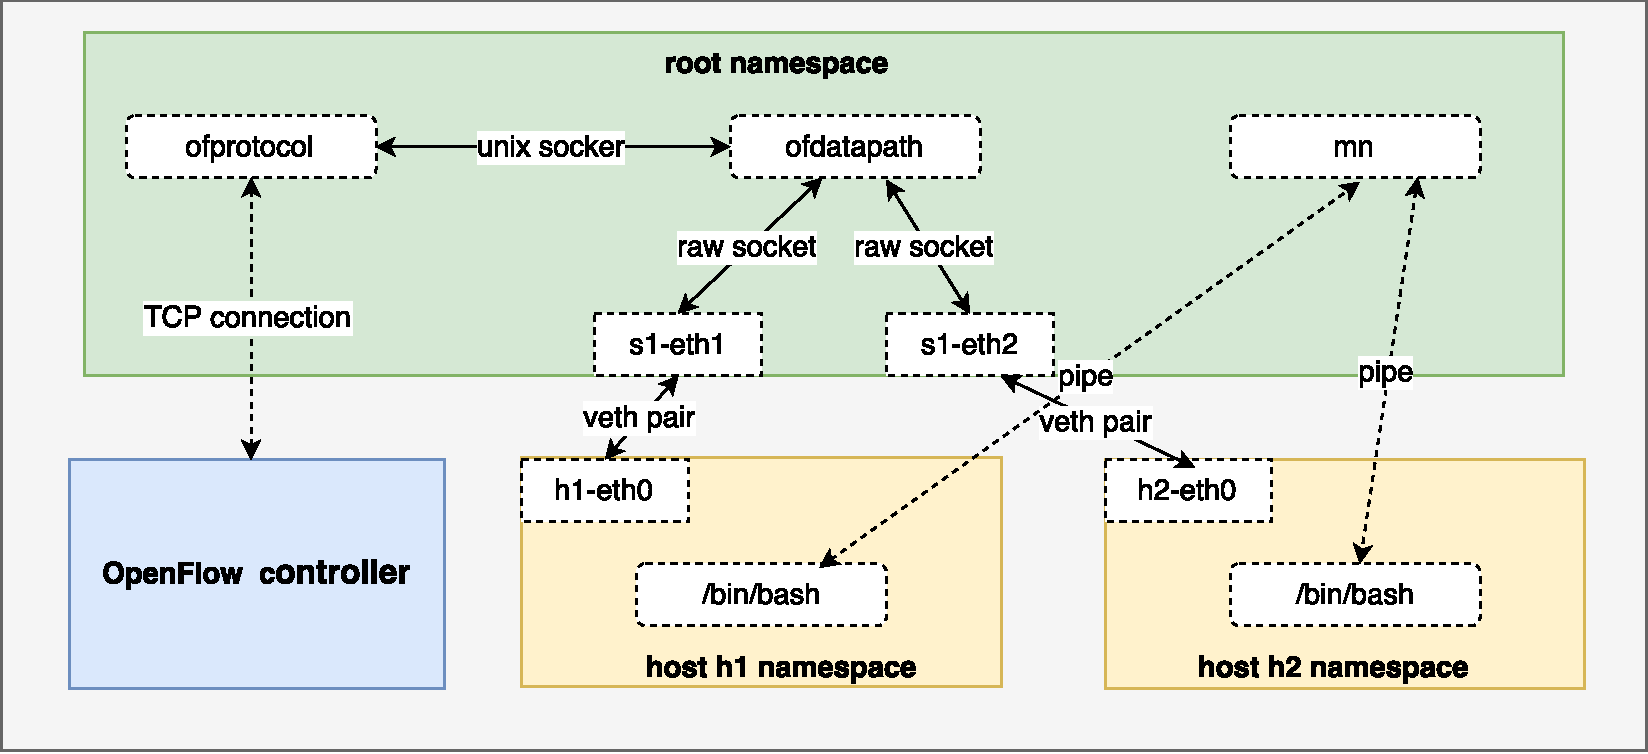
\includegraphics{mininet-components.pdf}}
	\caption{Mininet components \cite{Lantz:2010:NLR:1868447.1868466}.}
	\label{fig:mincomponent}
\end{center}
\end{figure}

Mininet uses the built-in Linux OS kernel's lightweight virtualization mechanism. It uses different useful Linux features like network namespaces, process groups, and CPU bandwidth isolation and combines them with virtual Ethernet links and link schedulers. These in-build features of Linux helps Mininet to start faster and also gives flexibility to scale the system with hundreds of hosts and switches on a single machine. This is not possible in emulators which use full virtual machines \cite{Lantz:2010:NLR:1868447.1868466}. A Mininet network consists the following components (see Figure \ref{fig:mincomponent}):

\paragraph{Network Namespace:}
Network namespaces are the container \cite{container} for network state. It provides processes (or group of processes) with exclusive ownership of interfaces, ports, and routing tables (such as ARP and IP). With network namespace, one can have different and separate instances of network interfaces and routing tables that operate independently of each other \cite{Handigol:2012:RNE:2413176.2413206}.

\paragraph{Hosts:}
A Mininet host is basically a shell process (e.g., bash) moved into its own network namespace with the unshare (CLONE NEWNET) system call. Each Mininet host has its own virtual Ethernet interface(s) and a pipe to a parent Mininet process (i.e., mn)(see Figure \ref{fig:mincomponent}), which sends commands and monitors output. Mininet uses Linux functionality of hierarchical scheduling, resource management, and CPU Bandwidth limiting features to limit the fraction of a CPU available to each process group \cite{cgroups-man} \cite{Handigol:2012:RNE:2413176.2413206}.

\paragraph{Links:}
A Mininet Link is basically a virtual Ethernet pair or veth pair\cite{container}. It acts like a wire connecting between two virtual interfaces. Each interface acts like a fully functional ethernet port to all systems and application software. Packets sent through one interface are delivered to the other interface of the veth pair. A veth pair may be attached to virtual switches such as the Linux bridge or an OpenFlow software switch. The data rate of each link can be configured, which is achieved by using Linux Traffic Control (\textit{tc}) \cite{tc-man}, which has a number of packet schedulers to shape traffic to a configured rate \cite{Handigol:2012:RNE:2413176.2413206}.

\paragraph{Switches:}
Mininet typically uses the default Linux bridge or Open vSwitch running in kernel mode to switch packets between interfaces. These software OpenFlow switches provide similar packet delivery facilities that would be provided by a hardware switch. Both user-space and kernel-space switches are available. Usually switch runs in the kernel for better speed \cite{Handigol:2012:RNE:2413176.2413206}.

\paragraph{Controllers:}
Mininet Controllers can be an external or internal process running anywhere on the real or simulated network. The controller should provide IP-level connectivity to the machine on which the Mininet switches are running. For example, for Mininet running in a VM, the controller could run inside the VM, natively on the host machine, or in the cloud \cite{Handigol:2012:RNE:2413176.2413206}.

\subsubsection{Mininet Advantages}
Mininet combines many of the best features of simulators, emulators, and real network testbeds \cite{min-over}.
\begin{itemize}
	\item Starting up a simple Mininet network takes just a few seconds.
	\item Mininet allows creating custom topologies, e.g., a data center network, large Internet-like topologies, or a simple single switch network.
	\item It is possible to run any real programs (e.g., a web server, TCP monitoring tool, or Wireshark) that can be run on Linux.
	\item It is simple to create and run Mininet experiments by writing simple (or complex) Python scripts.
	\item Mininet's switches are programmable using the OpenFlow protocol, so one can easily develop a custom SDN controller and implement customized packet forwarding logic as necessary.
	\item Mininet can be run on a laptop, on a server, or in a VM.
	\item Mininet provides a straightforward and extensible Python API for network creation and experiments.
	\item Mininet has a Command Line Interface (CLI) that is topology-aware and OpenFlow-aware; thus, very useful for debugging or running network-wide tests.
	\item Mininet provides a simple and inexpensive network testbed for developing and testing OpenFlow network applications.
	\item There is an active community mail-group for discussion about various features and problem about Mininet.
\end{itemize}


\subsubsection{Mininet Limitations}
Mininet is a great tool for networking experiments, but it does have some limitations as well \cite{min-intro}.
\begin{itemize}
	\item Mininet has a resource limitation concern. Mininet-based networks currently cannot exceed the CPU or bandwidth available on a single machine. This problem can be resolved in MaxiNet, which is described in section \ref{maxinet}.
	\item Mininet, currently, cannot run non-Linux compatible OpenFlow switches or applications. Software that depends on BSD, Windows, or other operating system kernels can not be run on Mininet.
	\item All Mininet hosts share the host file system and PID space. The user has to be careful with the daemon process running on Mininet host, if they require configuration in /etc or in shared common place.
	\item It is not easy to use virtual time in Mininet to achieve faster than real-time results, such as in simulation.
	\item One has to write own OpenFlow controller if custom routing or switching behavior is needed in the network. It is, however, easy to combine any OpenFlow controller to run with Mininet network.
\end{itemize}

\subsection{MaxiNet}\label{maxinet}
MaxiNet is a highly scalable, distributed emulation environment for large SDNs \cite{max-over}. MaxiNet is basically an extension of the Mininet emulation environment. Mininet has a drawback of not being able to run across multiple physical machines and for this reason, Mininet is not highly scalable. MaxiNet resolves these problems by distributing nodes between multiple physical hosts. MaxiNet achieves the distributed functionality by running on a cluster of several physical machines (called \textit{Worker}) connected by a physical network. Through this, MaxiNet distributes a part of the whole network between these workers and each of these workers runs a Mininet emulation on it. MaxiNet uses Generic Routing Encapsulation (GRE) tunnels to interconnect switches and hosts spread across different workers. The workers communicate through the physical network to pass traffic across the workers. By using MaxiNet, a large virtual network of thousands hosts and switches can be emulated with multiple numbers of workers. MaxiNet coordinates between these isolated Mininet emulation using a centralized API invoked in a specially-designed worker called \textit{Frontend}. The main job of the frontend is to partition the whole network into smaller units and distribute these smaller networks into the workers. Frontend also keeps track of which node resides on which worker. This way, one can easily access all nodes through the frontend. The frontend can also be configured to act as a worker and it has to be done manually before starting the experiment. Through this, MaxiNet allows emulating very large SDN testbed in a very convenient way \cite{6857078}.

\begin{figure}[tb]
\begin{center}
	\resizebox{\textwidth}{!}
	{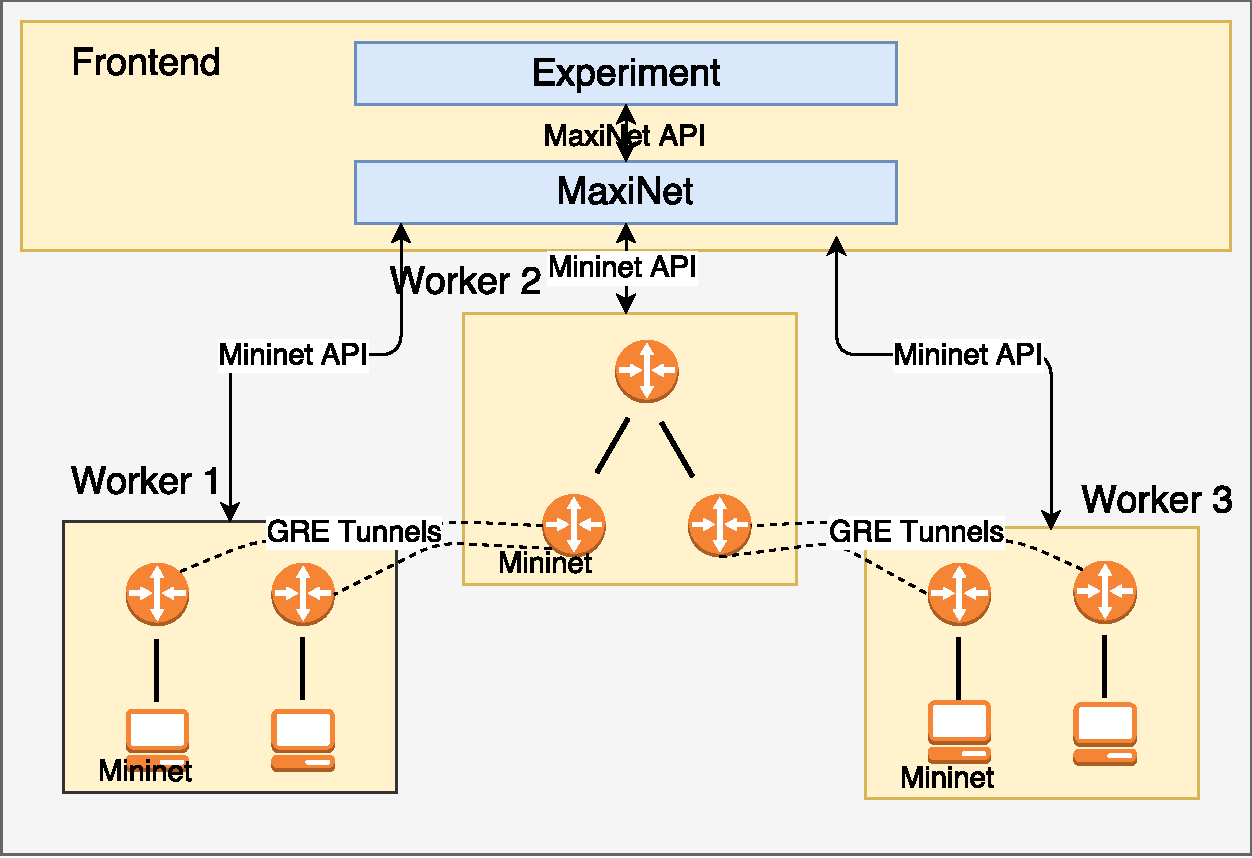
\includegraphics{maxinet-overview.pdf}}
	\caption{Schematic view of MaxiNet \cite{6857078}.}
	\label{fig:maxoverview}
\end{center}
\end{figure}

Figure \ref{fig:maxoverview} shows the schematic view of MaxiNet. A user provides a topology to the MaxiNet Experiment in the frontend to set up a network. The Experiment uses MaxiNet API to pass that information to MaxiNet. MaxiNet partition that topology into several smaller virtual network to distribute among the workers. MaxiNet uses the graph partitioning library METIS \cite{Karypis95metis--} for partitioning. METIS computes the partitions, dividing the total nodes almost equally among the workers. The aim of the partitioning process is to restrain most of the emulated traffic locally to the workers. Each MaxiNet worker takes these divided units assigned to them and instantiate a Mininet network in their system. MaxiNet uses Mininet API to control the workers and uses RPC calls to communicate with them. The worker uses GRE tunnels to communicate among the nodes between them. MaxiNet API can be used to set up, control, and shut down a virtual network and it is designed similarly to Mininet API to ease the use of MaxiNet among Mininet users \cite{6857078}.
 
\subsubsection{MaxiNet Advantages and Limitations}
Since MaxiNet is a distributed enhancement of Mininet it has similar advantages and disadvantages to Mininet. One major advantage of MaxiNet is it can be scalable up to thousands of nodes (switches and hosts) and can be distributed among multiple physical machines. However, as a disadvantage, its CLI support is not vast; it would have been helpful to have all Mininet command supported in MaxiNet. The data rate between nodes on different workers is very less compared to the nodes on same worker. Its documentation is poor but not a major drawback as there are many support groups available for Mininet.

\subsection{Ryu SDN Framework}\label{sec:ryu}
Ryu is a component-based open source platform for building SDN applications. Ryu is designed based on the philosophy of agility and flexibility in mind; thus, it is easy to manage. Ryu supports various protocols for managing network devices, such as OpenFlow (1.0, 1.1, 1.3, 1.4, 1.5), NetCONF, and OF-config, among others. Ryu provides software components with well-defined APIs. It is easy for developers to create new network management and controller applications using Ryu. One can easily modify an existing component and build a new component or implement his own component. It is easy to combine multiple Ryu components and build a Ryu application based on the specific requirements of a developer to ensure that the underlying network can meet the demands. A component of Ryu is basically separation functional unit and they communicate by passing messages instead of directly referencing each other. Existing components of Ryu are implemented in Python and a component consists of python thread or OS process \cite{ryu}. Figure \ref{fig:ryufwis} shows how Ryu framework fits in the SDN.

\begin{figure}[tb]
\begin{center}
	\resizebox{\textwidth}{!}
	{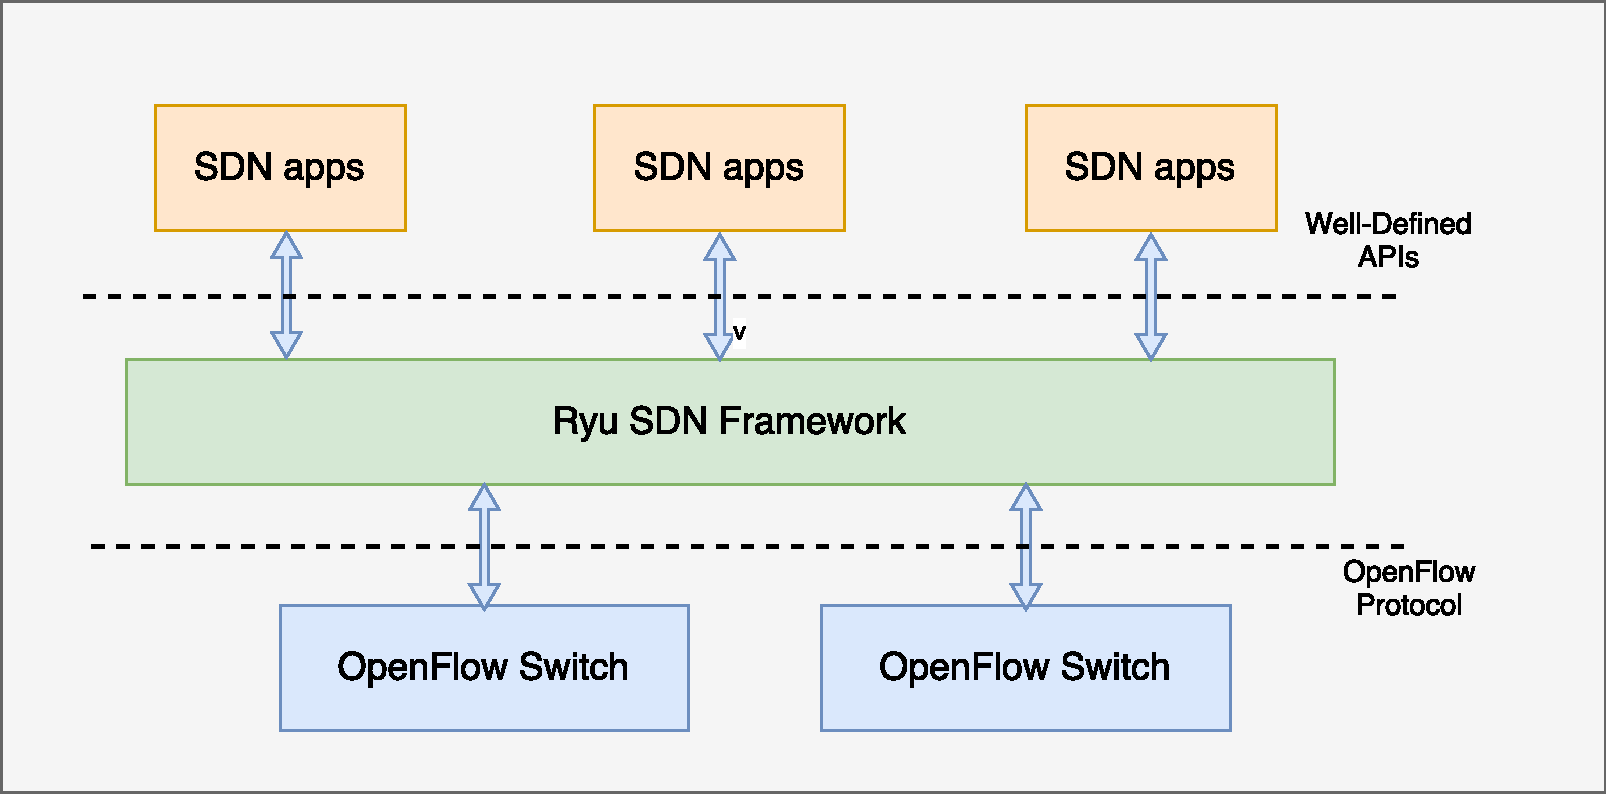
\includegraphics{ryu-frameworkinsdn.pdf}}
	\caption{Ryu framework in SDN.}
	\label{fig:ryufwis}
\end{center}
\end{figure}

As part of this study, a controller application is developed using some of the components of Ryu SDN framework. It uses OpenFlow 1.3 to interact with the forwarding plane (switches and routers) to modify how the network will handle traffic flows. Some Ryu component descriptions used in the SDN controller of the testbed are listed below.

\paragraph{ryu.base.app\_manager:}
This is the central management of a Ryu application. It is responsible for loading the application, providing context to the application, and routing messages between Ryu applications.
\paragraph{ryu.controller.controller:}
This is the main component of an OpenFlow controller. It handles connections from the switches and generate events and route them to appropriate entities like Ryu applications.
\paragraph{ryu.controller.dpset:}
This manages switches.
\paragraph{ryu.controller.ofp\_event:}
This is the class for OpenFlow event definitions.
\paragraph{ryu.controller.ofp\_handler:}
This is the handler of basic OpenFlow handling including negotiation.
\paragraph{ryu.ofproto.ofproto\_v1\_3:}
This is the class for OpenFlow 1.3 definitions.
\paragraph{ryu.ofproto.ofproto\_v1\_3\_parser:}
This module implements OpenFlow 1.3.x.
\paragraph{ryu.topology:}
This is the Switch and link discovery module.

\subsubsection{Ryu Application Programming Model}
This section explains the Ryu application programming model (see Figure \ref{fig:ryuarch}). To understand the SDN Controller (see Section \ref{sec:fca}) flow developed for this study, it is important to know the Ryu application programming model \cite{ryuapm}.

\begin{figure}[H]
	\begin{center}
		\resizebox{\textwidth}{!}
		{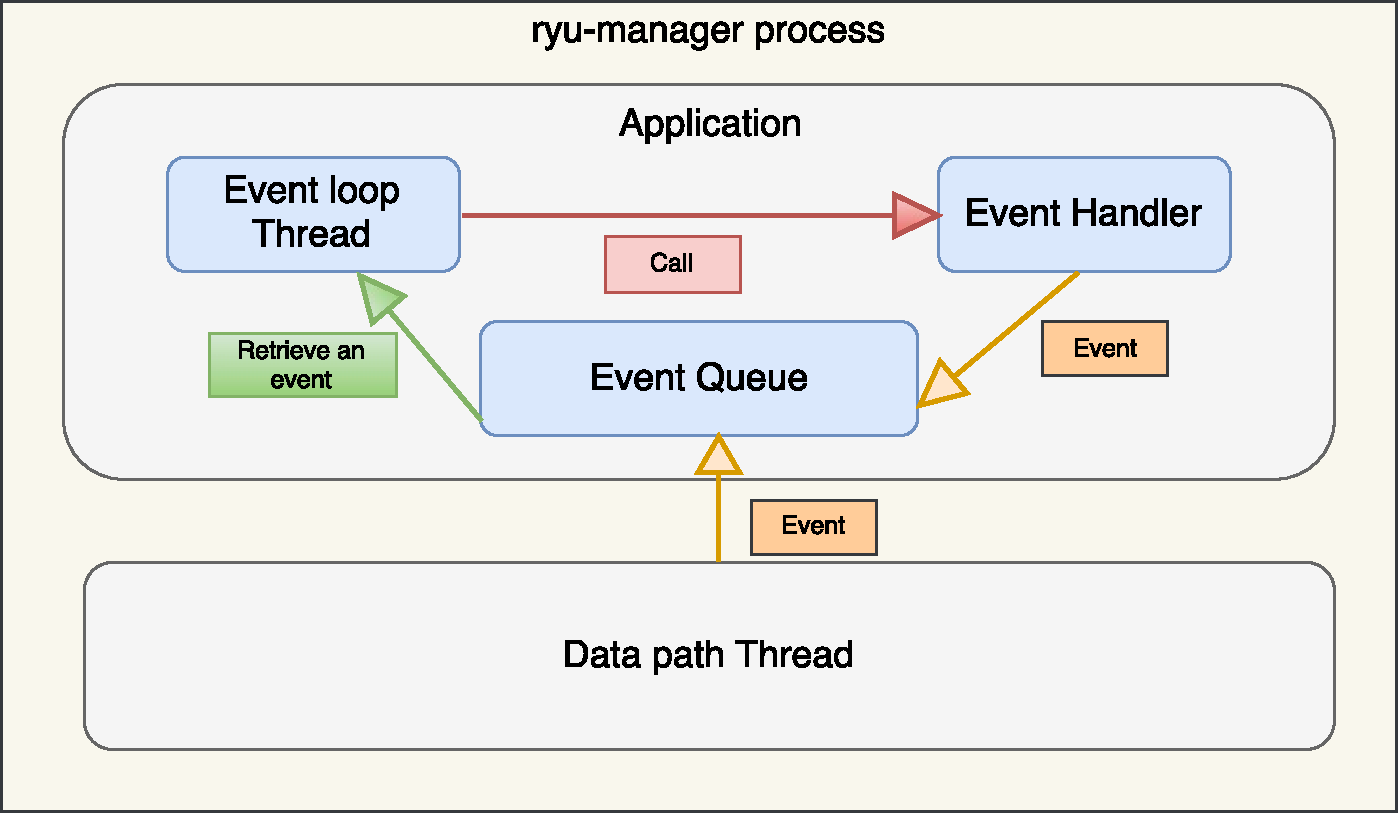
\includegraphics{ryu-architecture.pdf}}
		\caption{Ryu application programming model.}
		\label{fig:ryuarch}
	\end{center}
\end{figure}

\paragraph{Applications:}
Applications are a subclass of \textit{ryu.base.app\_manager.RyuApp}. Ryu applications are single-threaded entities which implement various functionalities in Ryu. User logic is supposed to be implemented as an application.
\paragraph{Event:}
Ryu applications communicate between them, transmitting and receiving events. Events are the objects of a class that inherits \textit{ryu.controller.event.EventBase}. Ryu events can also contain arbitrary python objects.
\paragraph{Event Queue:}
Each Ryu application has a receive queue for receiving events. The queue is implemented as FIFO and retains the order of events.
\paragraph{Event Loop Thread:}
Ryu application runs a thread for event processing from the event queue. The thread runs a loop whenever there is an event available in the queue. The event loop will load the events and will call the appropriate event handler for processing the event type.
\paragraph{Datapath Thread:}
Datapath thread is used to describe the connection of the OpenFlow switch with a controller. It is an instance of the class \textit{ryu.controller.controller.Datapath}. Threads and queues in Ryu are implemented with python eventlet/greenlet package.
\paragraph{Event Handlers:}
An event handler is a method in the user application class using the decorator \textit{ryu.controller.handler.set\_ev\_cls}. Application events loop queued events from the event queue and the defined event handler is called.
\paragraph{ryu-manager:}
This is the main executable to start a Ryu application. It instantiates the single instance of class \textit{ryu.base.app\_manager.AppManager}. This internally loads Ryu applications, create contexts to Ryu applications, and start the services.

\subsection{Iperf and Socat}
Iperf is a tool normally used for measuring the throughput of the network. It can create Transmission Control Protocol (TCP) and User Datagram Protocol (UDP) data streams, which are used to measure the throughput. It is developed in C and has both client (to generate traffic) and server (to discard traffic) functionality and able to measure throughput between any connected two ends of network unidirectionally or bi-directionally. It can generate controlled traffic (UDP mode) for a specified duration. It is an open source, cross-platform tool and can be used for both wired and wireless networking equipment testing \cite{iperf}. Iperf supports various parameters for testing a network, or for optimizing or tuning a network. The controlled data stream generation functionality of iperf is used for generating traffic in the emulation testbed (see Figure \ref{fig:emulator}) \cite{iperfman}.

Socat is a command line based powerful utility with many features. It can establish two bidirectional byte stream for reading or writing data between two ends. It can be used for almost any kind of data transferring between any kind of stream. Socat supports a various feature like redirection of TCP, UDP, and SCTP ports to other sites; execution of commands; start a child process and much more, it is a Switch knife for the user. It is used as a data sink in the CA for receiving data along with its child process creation facility to resend the received packet back to the data source (see Figure \ref{fig:emulator}) \cite{socatman}.

\subsection{Tc and NetEm} \label{sec:tan}
Tc is used to configure Traffic Control in the Linux kernel. Traffic Control is used to specify the sets of queuing systems and mechanisms by which packets are received and transmitted in the network. Its functionality can be used in deciding which packet to accept or transmit, in what order, and at what rate on the input or output of a network interface \cite{howtc}. This section of description is mainly based on the tc and netem man page \cite{tc-man} \cite{netemman}. Traffic Control consists of the following operations:

\begin{itemize}
	\item SHAPING, to control the rate of egress traffic.
	\item SCHEDULING, to improve the interactivity for egress traffic.
	\item POLICING, to limit the ingress traffic as opposed to shaping.
	\item DROPPING, to discard both on ingress and on egress.
\end{itemize}

The processing of traffic is controlled by three kinds of objects: qdiscs, classes, and filters.
\paragraph{QDISCS:} Qdisc is an abbreviation for `queueing discipline'. Kernel always enqueues packets to the qdisc configured for an interface to send a packet to it. There are two types of qdiscs. One is the classful qdiscs (e.g., pfifo, bfifo, pfifo\_fast, red, sfq, tbf), which can contain classes and provide a handle to attach filters. Another is the classless qdiscs (e.g., CBQ, HTB, PRIO) which do not contain classes, making it impossible to attach a filter. Normally, the simple classful qdisc pfifo, which does no processing at all and is a pure First In, First Out queue, is the default.
\paragraph{CLASSES:} Classful qdiscs can contain classes, which contain further qdiscs. Traffic may then be enqueued in any of the inner qdiscs, which are within the classes.
\paragraph{FILTERS:} A filter is used by a classful qdisc to determine in which class a packet will be enqueued. On the arrival of traffic, it needs to be classified and the filter is one method to classify it. Filters reside within qdiscs and does not govern any event. All filters attached to the class are called until one of them returns with a match.

While in operation, classes form a tree and each class has a single parent. A class may have multiple children. Qdiscs CBQ, and HTB allow for runtime addition of classes while PRIO is created with a static number of children. Qdiscs, which allow dynamic addition of classes, can have zero or more subclasses to which traffic may be enqueued. Furthermore, each class contains a leaf qdisc which by default has pfifo behavior, although another qdisc can be attached in place. When a packet enters a classful qdisc, it can be classified based on three criteria (i.e., tc filter, Type of Service, and skb-priority) to one of the classes within. Each node within the tree can have its own filter, but higher level filters may also point directly to lower classes. If classification does not succeed, packets are enqueued to the leaf qdisc attached to that class.

NetEm is an enhancement of the Linux traffic control facility that allows adding delay, packet loss, duplication, and other characteristics to packets outgoing from a selected network interface. NetEm is built using the existing Quality Of Service (QOS) and Differentiated Services (diffserv) facilities in the Linux kernel.

For the purpose of this study, Linux Traffic Control functionality with NetEm (to add delay) for emulating the processing capability in CAs is used. Its implementation is further discussed in Section \ref{sec:tmfg}.          % Chapter 2
% chap3.tex (Implementation)

\chapter{Implementation}\label{IMPL-CHAP}
In section \ref{sec:pd}, I discussed the different problems I need to solve and in chapter \ref{BACK-CHAP}, I have discussed the different tools and technologies I used in this thesis. Here, I will talk about how I solved those problems using said tools, particularly the implementation details of each individual components or events (e.g., testbed setup, traffic generation), and will describe the execution workflow of the emulation.

\begin{figure}[H]
	\begin{center}
		\resizebox{\textwidth}{!}
		{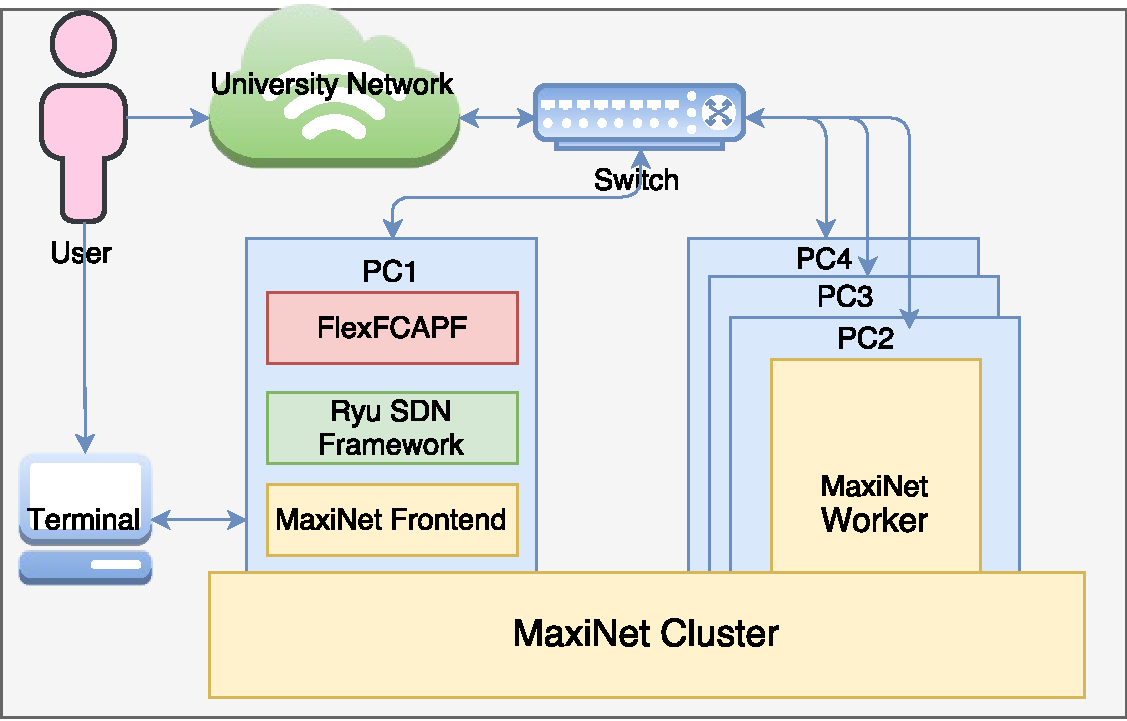
\includegraphics{testbed-infrastructure.pdf}}
		\caption{Overview of testbed infrastructure.}
		\label{fig:testinfra}
	\end{center}
\end{figure}

After selecting the tools and technology, I have to prepare a laboratory setup design, i.e., where to place which components. Figure \ref{fig:testinfra} depicts the overview of the current testbed infrastructure. The testbed consists of four physical machines (PC1, PC2, PC3, and PC4). All four machines are connected to Paderborn University's network with an ethernet switch (20Gbits) using their internal Network Interface Cards (NICs). A terminal is connected to the first machine. A user can access the testbed using the terminal or by using ssh via the university network. PC1 is used as MaxiNet frontend and the other three machines are used as MaxiNet workers. FlexFCAPF and Ryu SDN Framework also run on PC1. These machines altogether build the MaxiNet Cluster.

Before I describe the detailed implementation, it is important to understand the emulation's functional overview, its components, and how they communicate with each other. Figure \ref{fig:testcomp} shows the components of the emulation and how they work together. The emulation is logically divided into four functional modules in high level as follows:
\begin{enumerate}
\item External Module - the Topology Generator and the DFG Generator components fall in this module. Topology Generator communicates with the emulation through input file sharing (topology description). DFG Generator is part of the emulation execution process; it creates DFG dynamically based on some defined parameter (load level, scale). The emulation execution then inserts the DFG into the testbed for further processing.
\item SDN Controller Module - the Ryu SDN controller application is a component of this module and the implementation of a customized SDN controller to match the specific requirement of the emulation is also done under this functional module. The SDN controller communicates with the underlying network elements (switch/router) via TCP socket connection and opens up REST API for FlexFCAPF to communicate with it.
\item Emulator Module - the emulation framework (MaxiNet or Mininet) comes under this module; the network elements (switch/router, host, and links) creation are also implemented under this functional module. Each switch/router is connected to a host, via a link (basically veth pair), and each host running a shell to execute a command on it. Each host has a pipe connected to the emulation framework's parent process (i.e., an instance of the network emulator).
\item FlexFCAPF Module - FlexFCAPF algorithm is implemented as part of this module. The complete FlexFCAPF algorithm is implemented in a class named \textit{CPFlex}. The network emulation instance is a member of the CPFlex class; that way, the CPFlex class instance has direct access to the network. Real traffic generation and data flow processing are also implemented as part of this module.
\end{enumerate}

\begin{figure}[H]
	\begin{center}
		\resizebox{\textwidth}{!}
		{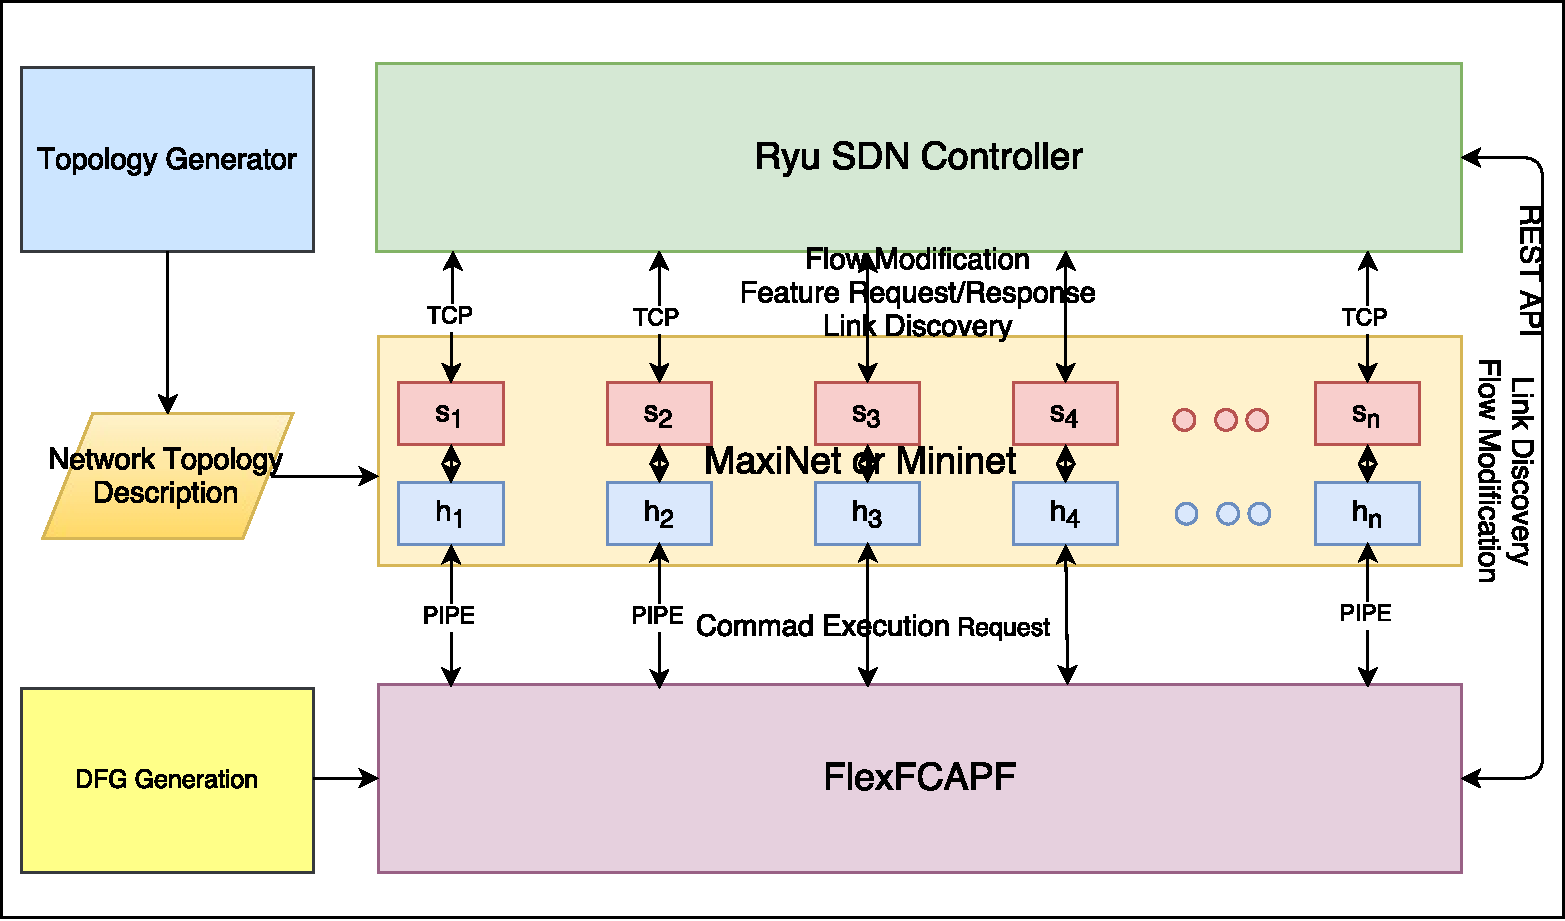
\includegraphics{testbed-components.pdf}}
		\caption{Overview of testbed components.}
		\label{fig:testcomp}
	\end{center}
\end{figure}

The implementation of all the components of each module is discussed in the following sections.

\section{External Module}\label{sec:el}
The emulation needs a topology description to create its underlying network testbed. The topology description is basically the arrangement of network elements of the testbed, e.g., nodes, edge. I am using a python script provided by my supervisor to generate topology description file. It can generate two types of topology, i.e., Mesh and Ring.

Emulation uses similar traffic generation model like the simulation, mentioned in \cite{7343600}. 

The simulation uses a non-stationary Poisson process with $\lambda = |V| \times loadlevel(t)$ and implemented using the thinning method \cite{Law:1999:SMA:554952} for DFG generation. While generating traffic, a daily load level curve (see Figure \ref{fig:24loadlevel}) is followed based on the cellular data traffic characteristics explained in \cite{Zhang:2012:UCC:2342468.2342472}. In emulation, the same model for traffic generation is used with a modified $\lambda = |V| \times loadlevel(t, scaling)$. Load level factor $scaling$ is used to set the scaling of the load level due to the hardware resource limitation in the testbed environment.

\begin{figure}[H]
	\begin{center}
%		\resizebox{\textwidth}{!}
		{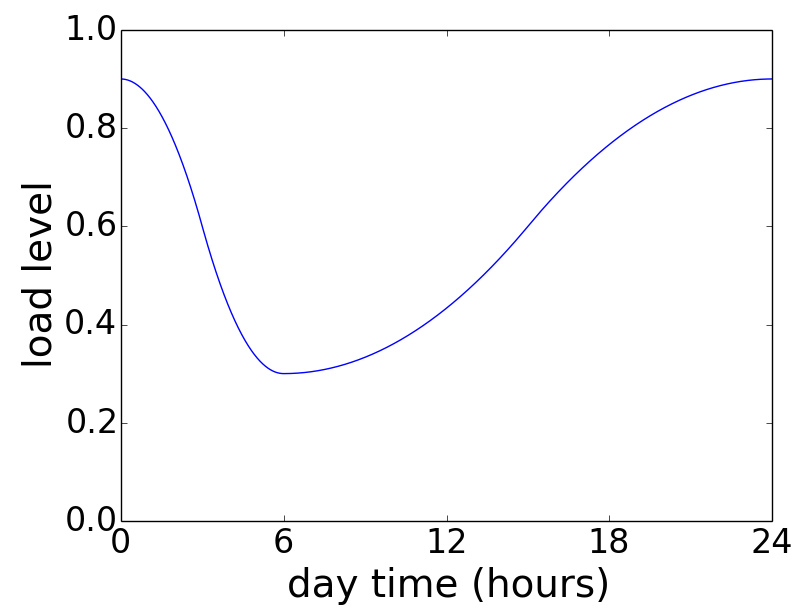
\includegraphics[width=0.40\textwidth]{24-loadlevel.png}}
		\caption{Daily load curve \cite{7343600}.}
		\label{fig:24loadlevel}
	\end{center}
\end{figure}

\section{SDN Controller Module}\label{sec:fca}
Ryu SDN Controller is the component of this module which I developed as part of this study. The SDN controller has mainly two jobs to fulfill, i.e., provide underlying network link details to FlexFCAPF whenever it requests and modifies the forwarding entries in the network elements the way FlexFCAPF wants.

\paragraph{REST Interface Implementation:}
The SDN controller provides a REST interface for serving the request of FlexFCAPF. The Ryu framework has a web server function corresponding to the Web Server Gateway Interface (WSGI). It specifies how a web server can communicate with a web application, and how web applications can be tied together to process one request \cite{wsgi}. By using this functionality, it is possible to create a REST API \cite{ryu}. Ryu has a component \textit{ryu.app.wsgi} which implements that functionality to create REST API.


\begin{lstlisting}[caption={REST API implementation},label={lst:rai},language=Python,tabsize=2,basicstyle=\footnotesize,breaklines=true, showspaces=false,showstringspaces=false,showtabs=false,frame=single]
class ControllerRequestProcessor(ControllerBase)
	def __init__(self, req, link, data, **config):
		super(ControllerRequestProcessor, self).__init__(req, link, data, **config)
		self.fcapf_network_controller = data[fcapp_controller_instance]
	@route('fcapfnetworkcontroller', '/fcapfnetworkcontroller/topology/links', methods=['GET'])
	def list_links(self, req, **kwargs):
		return self._links(req, **kwargs)
\end{lstlisting}

Listing \ref{lst:rai} shows how I implemented REST API in testbed SDN controller. The testbed SDN controller has a class \textit{ControllerRequestProcessor}, it accepts HTTP requests to be processed by Ryu REST AP and is a subclass of \textit{ryu.app.wsgi.ControllerBase}. This way, FlexFCAPF may send the HTTP request to the SDN controller to avail the facility provided by REST API. First, the method \textit{list\_links} is associated with a URL so that the method can be called by HTTP request. It is implemented by a decorator \textit{route} defined in Ryu. The content specified by the decorator have three arguments; the first argument is any name, the second argument is to specify the URL, and the third argument is to specify the HTTP method (e.g., PUT, GET).

\paragraph{Link Discovery Implementation:}
Ryu uses an SDN mechanism called OFDP (OpenFlow Discovery Protocol) to support topology discovery in the network \cite{ofdp}. OFDP internally uses the Link Layer Discovery Protocol (LLDP) \cite{5251812} with slight modifications to perform topology discovery in an OpenFlow network. LLDP allows a network station to advertise their capabilities to other neighbor's station. Ryu has a component called \textit{ryu.topology.api} which is basically the switch and link discovery module of Ryu. I used that module in the testbed SDN controller to retrieve the link details of the network and prepare JSON formatted string and send it to the requesting FlexFCAPF (see Listing \ref{lst:ldr}).

\begin{lstlisting}[caption={Link discovry request},label={lst:ldr},language=Python,tabsize=2,basicstyle=\footnotesize,breaklines=true, showspaces=false,showstringspaces=false,showtabs=false,frame=single]
def _links(self, req, **kwargs):
	dpid = dpid_lib.str_to_dpid(kwargs['dpid'])
	links = get_link(self.fcapf_network_controller, dpid)
	body = json.dumps([link.to_dict() for link in links])
	return Response(content_type='application/json', body=body)
\end{lstlisting}

\paragraph{Event Handler Implementation:}
Once a connection is established between the OpenFlow switch and an SDN controller, the controller can then configure and manage the switch (see Section \ref{par:ofc}). It receives events from the switch and sends packets out to the switch. These handshake procedures are taken care by the Ryu framework itself. The controller usually sends a features request message to know the capabilities of the switch and the switch responds with a features reply message. This is commonly performed upon establishment of the OpenFlow channel \cite{ryubook}. For that purpose, the controller has to save the connection information to access the switch. In Ryu, when an OpenFlow message is received, an event corresponding to the message is generated. I implemented an event handler in the controller corresponding to the desired message to be received as shown in Listing \ref{lst:ehi}. Upon receiving the Switch Features (i.e., features reply from the switch) message in the controller, the \textit{Datapath} object is retrieved and saved for future reference along with the DPID. The \textit{Datapath} class is mainly responsible for actual communication with the OpenFlow switch.


\begin{lstlisting}[caption={Event handler implementation},label={lst:ehi},language=Python,tabsize=2,basicstyle=\footnotesize,breaklines=true, showspaces=false,showstringspaces=false,showtabs=false,frame=single]
class FCAPFNetworkController(app_manager.RyuApp):
	@set_ev_cls(ofp_event.EventOFPSwitchFeatures, CONFIG_DISPATCHER)
	def switch_features_handler(self, ev):
		datapath = ev.msg.datapath
		self.switches[datapath.id] = datapath
\end{lstlisting}

\paragraph{Flow Modification Implementation:}
Upon receiving the request for flow modification (add/delete) request from FlexFCAPF, the SDN controller loop through all entries and modify the flow table in the switch. Initially, I implemented the controller wrongly, i.e., it used to receive one entry per request, but that strategy have a huge performance impact. This is because for each flow modification, FlexFCAPF has to establish an HTTP connection, send the request to the controller, and wait for the response. For a big network, FlexFCAPF has to modify hundreds of flow entries in the network every time a reconfiguration happens. Thus, I changed the logic to process bulk flow modification entries in the controller so that FlexFCAPF can send all flow addition entries in one request and all flow deletion entries in another request. This way, performance improved a lot.

Listing \ref{lst:paei} shows how I implemented the forwarding entry addition in the flow table of a switch. This part of code first converts the datapath id string to a 16-digit hex value defined by \textit{DPID\_PATTERN} of Ryu library. It uses the \textit{FCAPFNetworkController} instance to retrieve the datapath object matching the hex DPID. It is important to remember that the DPID and the datapath object mapping were saved during the features message handling. The input flow configuration entry is parsed and converted to the Ryu supported format. The controller uses action type \textit{ofproto\_v1\_3.OFPP\_NORMAL}, which means the packet will be forwarded by the L2/L3 switch function. A match object is generated calling the constructor of \textit{OFPMatchto} class based on the ethernet frame type (e.g., IP, ARP). Finally, priority 1 is set and the \textit{\_add\_flow} method is called to sent the Flow Mod message.

\begin{lstlisting}[caption={Processing add entry implementation},label={lst:paei},language=Python,tabsize=2,basicstyle=\footnotesize,breaklines=true, showspaces=false,showstringspaces=false,showtabs=false,frame=single]
def _set_flow_table(self, dpid_str, entry):
	dpid = dpid_lib.str_to_dpid(dpid_str)
	contr_inst = self.fcapf_network_controller
	datapath = contr_inst.switches.get(dpid)
	if action == 'normal':
		action = ofproto_v1_3.OFPP_NORMAL
	if datapath is not None:
		parser = datapath.ofproto_parser
		actions = [parser.OFPActionOutput(action)]
		if dl_type == "ip":
			port = entry['inport']
			match = parser.OFPMatch(in_port=port, ipv4_src=ip_src,ipv4_dst=ip_dest, eth_type=0x0800)
		elif dl_type == "arp":
			match = parser.OFPMatch(arp_spa=ip_src, arp_tpa=ip_dest, eth_type=0x0806)
		else:
			LOG.error("Wrong input!!")
		self._add_flow(datapath, 1, match, actions)
\end{lstlisting}

The processing of the forward entry addition is not done yet. The method \textit{\_add\_flow} set the instruction to use the \textit{ofproto.OFPIT\_APPLY\_ACTIONS} so that the specified action is immediately used. I created a class instance of \textit{OFPFlowMod} to prepare the modification message and the message is sent to the OpenFlow switch using the method \textit{datapath.send\_msg} call to add the forwarding entry in the flow table (see Listing \ref{lst:afei}).
\begin{lstlisting}[caption={Add forwarding entry implementation},label={lst:afei},language=Python,tabsize=2,basicstyle=\footnotesize,breaklines=true, showspaces=false,showstringspaces=false,showtabs=false,frame=single]
def _add_flow(self, datapath, priority, match, actions, buffer_id=None):
	parser = datapath.ofproto_parser
	inst = [parser.OFPInstructionActions(datapath.ofproto.OFPIT_APPLY_ACTIONS, actions)]
	mod = parser.OFPFlowMod(datapath=datapath, priority=priority, match=match, instructions=inst)
	datapath.send_msg(mod)
\end{lstlisting}
The deletion of forwarding entry from the flow table is similar to addition, therefore the description of that code which does the processing of deletion entry request is not presented. The difference is, while preparing forwarding entry modification message, here, a command \textit{ofproto.OFPFC\_DELETE} is used to specify the action of deleting forwarding entry while creating \textit{OFPFlowMod} class instance (see Listing \ref{lst:dfei}).
\begin{lstlisting}[caption={Delete forwarding entry implementation},label={lst:dfei},language=Python,tabsize=2,basicstyle=\footnotesize,breaklines=true, showspaces=false,showstringspaces=false,showtabs=false,frame=single]
def _del_flow(self, datapath, match):
	ofproto = datapath.ofproto
	parser = datapath.ofproto_parser
	mod = parser.OFPFlowMod(datapath, command=ofproto.OFPFC_DELETE, out_port=ofproto.OFPP_ANY, out_group=ofproto.OFPG_ANY,priority=1, match=match)
	datapath.send_msg(mod)
\end{lstlisting}

\section{Emulator Module}\label{sec:emmod}
The underlying network is the component of this module; the network can be created either using the MaxiNet or Mininet emulation framework. I started to implement the testbed with a small number of nodes using Mininet and tried prototyping experiments in Mininet. Later, I introduced MaxiNet in code and implement the whole process in a flexible manner. Since MaxiNet is based on Mininet, it was easy to keep both options available. One can choose either Mininet or MaxiNet while starting the experiment. The testbed network is created based on the user provided topology description files (see Section \ref{sec:el}). The \textit{CPFlex} instance takes the topology description file as input and converts it to an in-memory graph to represent the structure of the network using a user defined python class \textit{CrowdNetwork}. \textit{CrowdNetwork} internally uses the python package \textit{NetworkX} for storing the testbed structure in memory which I call FlexFCAPF network model. \textit{CrowdNetwork} class was developed by my supervisor as part of a simulation work. Network creation steps are similar for both MaxiNet and Mininet; only some API's are different. Here, I describe the common as well as the different network creation steps.

\subsection{Setup Network}\label{sec:setnet}
Listing \ref{lst:sni} shows how I set up the network using Mininet or MaxiNet. Both creates a \textit{Topo} object, a flexible empty topology (topo) with two parameters, \textit{TCLink} and \textit{CPULimitedHost}. \textit{TCLink} and \textit{CPULimitedHost} classes provide the option of setting limitation on link bandwidth, delay, loss, and host processing power. A standard naming convention for the host ($h_0 ... h_n$) and switch($s_0 ... s_n$) is followed. The standard is followed while assigning unique IP, MAC (to hosts), DPID, and listen port (to switches) as well. This standardization would help us track the hosts and switches. A node in FlexFCAPF model is represented by a host and a switch combination in the network. Switches are running in kernel level to get a better speed of communication between multiple hops in the network (see Section \ref{sec:mininet}). A host is attached to each switch to run some user-level process (e.g., flow generation). A link is added between the switch and its associated host and links are added for all the edges specified in FlexFCAPF model.
\begin{lstlisting}[caption={Setup network implementation},label={lst:sni},language=Python,tabsize=2,basicstyle=\footnotesize,breaklines=true, showspaces=false,showstringspaces=false,showtabs=false,frame=single]
def setupEmulationNetwork(self):
	topo = Topo(link=TCLink, host=CPULimitedHost)
	linkopts = dict()
	# Add switches and associated hosts
	s = 1
	for n in self.cn.G.node:
		hName = 'h' + str(n)
		hIp = Tools.makeIP(n + 1)
		hMac = Tools.makeMAC(n + 1)
		hObj = topo.addHost(name=hName, ip=hIp, mac=hMac)
		self.Hosts[hName] = {'obj': hObj, 'ip': hIp, 'mac': hMac}
		sName = 's' + str(n)
		sDpid = Tools.makeDPID(n + 1)
		sListenPort = (13000 + s - 1)
		switchopts = dict(listenPort=sListenPort)
		sObj = topo.addSwitch(name=sName, dpid=sDpid, **switchopts)
		self.Switches[sName] = {'obj': sObj, 'dpid': sDpid, 'listenport': sListenPort}
		s += 1
		topo.addLink(hObj, sObj, **linkopts)
	for key, value in self.cn.G.edges():
		sName1 = 's' + str(key)
		sName2 = 's' + str(value)
		sObj1 = self.Switches[sName1]['obj']
		sObj2 = self.Switches[sName2]['obj']
		topo.addLink(sObj1, sObj2, **linkopts)
\end{lstlisting}

\paragraph{Starting Network:}
This step is different for MaxiNet and Mininet since nodes are distributed across multiple physical machines in MaxiNet. MaxiNet first creates a cluster object and then pass the topo object along with the cluster object and switch parameter to create an \textit{Experiment} object. Finally, call the \textit{setup()} method using the experiment object to start the emulation. Whereas Mininet creates a Mininet object using the \textit{Topo} object, switch parameter and controller parameter and start the emulation network by calling the \textit{start()} method. The OpenFlow protocol version 1.3 is passed while creating Mininet network and the same is done for MaxiNet as well in a later step. Controller parameter with a value of \textit{RemoteController} is used so that the SDN controller may run anywhere on the network, but which must be started up and shut down manually or by some other mechanism outside of Mininet's direct control. MaxiNet by default run the controller with that option because MaxiNet internally starts multiple instances of Mininet and runs in a distributed environment. The Mininet network object or MaxiNet Experiment object is saved in a member variable of \textit{CPFlex} class for future reference. 

Listing \ref{lst:stni} shows the code implementation of the same.
 
\begin{lstlisting}[caption={Starting network implementation},label={lst:stni},language=Python,tabsize=2,basicstyle=\footnotesize,breaklines=true, showspaces=false,showstringspaces=false,showtabs=false,frame=single]
if self.emulator == "Mininet":
	# Mininet
	switch = functools.partial(OVSSwitch, protocols='OpenFlow13')
	net = Mininet(topo=topo, switch=switch, controller=RemoteController, host=CPULimitedHost, link=TCLink)
	net.start()
	# Save the Mininet object for future reference
	self.TestbedNetwork = net
elif self.emulator == "MaxiNet":
	# MaxiNet
	cluster = maxinet.Cluster()
	exp = maxinet.Experiment(cluster, topo, switch=OVSSwitch)
	exp.setup()
	# Save the Experiment object for future reference
	for switch in exp.switches:
		exp.get_worker(switch).run_cmd('ovs-vsctl -- set Bridge %s ' % switch.name + 'protocols=OpenFlow10,OpenFlow12,OpenFlow13')
	self.TestbedNetwork = exp
else:
	exit(1)
\end{lstlisting}

\paragraph{Running User Process:}
One important requirement of the emulation is to emulate a way to achieve data processing capability in the network. To achieve that functionality, a user process needs to be run in the Mininet/MaxiNet host, which is assigned as an LCA. The job of that process is to work as a packet receiver or sink and resend the received packet back to the source. Each Mininet/MaxiNet host is essentially a bash shell process attached to one or more network interfaces, so the easiest way to interact with it is to send input to the shell using the \textit{cmd()} method. I used that facility to run \textit{socat} listener process in each potential LCA host to receive the flow in the LCA. A \textit{/bin/cat} is executed by the \textit{socat} to resend the packet back to the source. Listing \ref{lst:rupi} shows the code implementation for the same.

\begin{lstlisting}[caption={Running user process implementation},label={lst:rupi},language=Python,tabsize=2,basicstyle=\footnotesize,breaklines=true, showspaces=false,showstringspaces=false,showtabs=false,frame=single]
for n in self.cn.G.node:
	if n in self.cn.C:
		hName = 'h' + str(n)
		hObj = self.TestbedNetwork.get(hName) if self.emulator == "Mininet" else self.TestbedNetwork.get_node(hName)
		hObj.cmd("socat -T 5 UDP-LISTEN:5001,fork,reuseaddr EXEC:\'/bin/cat\' &")
\end{lstlisting}

Here, the socat instance running on the LCA host acts as receiver of the packet as well as the generator of the duplicate packet to resend. The socat server instance keeps listening to port 5001 (the default port for iperf connection) continuously and waits for the client connection. When a client connection request comes in, the socat starts a child process to serve that client. One important point to notice here is the parameter \textit{-T} for specifying inactivity timeout. Initially, I was not using it and due to that, there were many child processes that keep running for hours even though the client (iperf) from the other end stopped sending packets. This ate up a lot of system resources and slowed down the complete processing. Introducing this timeout solve that problem. When socat is already in the data receiving loop and nothing has happened (no data arrived, no interruption occurred) for the timeout seconds, then the serving child process terminates. But the parent socat process stays alive to accept connection. Since I am using UDP traffic, this functionality is very useful for terminating the remote server as UDP cannot transfer EOF (see Section \ref{sec:tragen}).

\section{FlexFCAPF Module}
The components of this module are FlexFCAPF algorithm, routing table modification, traffic flow generation, and data flow processing (partially). FlexFCAPF algorithm was implemented as part of simulation evaluation, therefore, I will skip the detailed code-level description. However, it is important to know how the algorithm works to understand the complete emulation so I give an overview of the algorithm.

\subsection{FlexFCAPF Algorithm} \label{sec:algoadap}
In this section, I describe how FlexFCAPP algorithm works. Functionality wise, the complete algorithm has two parts. First is the initial controller placement functionality of FlexFCAPF, and second, the flexible reassignment functionality. To provide an initial overview, Figure \ref{fig:flexfcpfflow} outlines the key aspects of FlexFCAPF in a flow chart. This algorithm description is prepared based on the implementation of the algorithm specified in \cite{7343600}.

\begin{figure}[H]
\begin{center}
	\resizebox{\textwidth}{!}
	{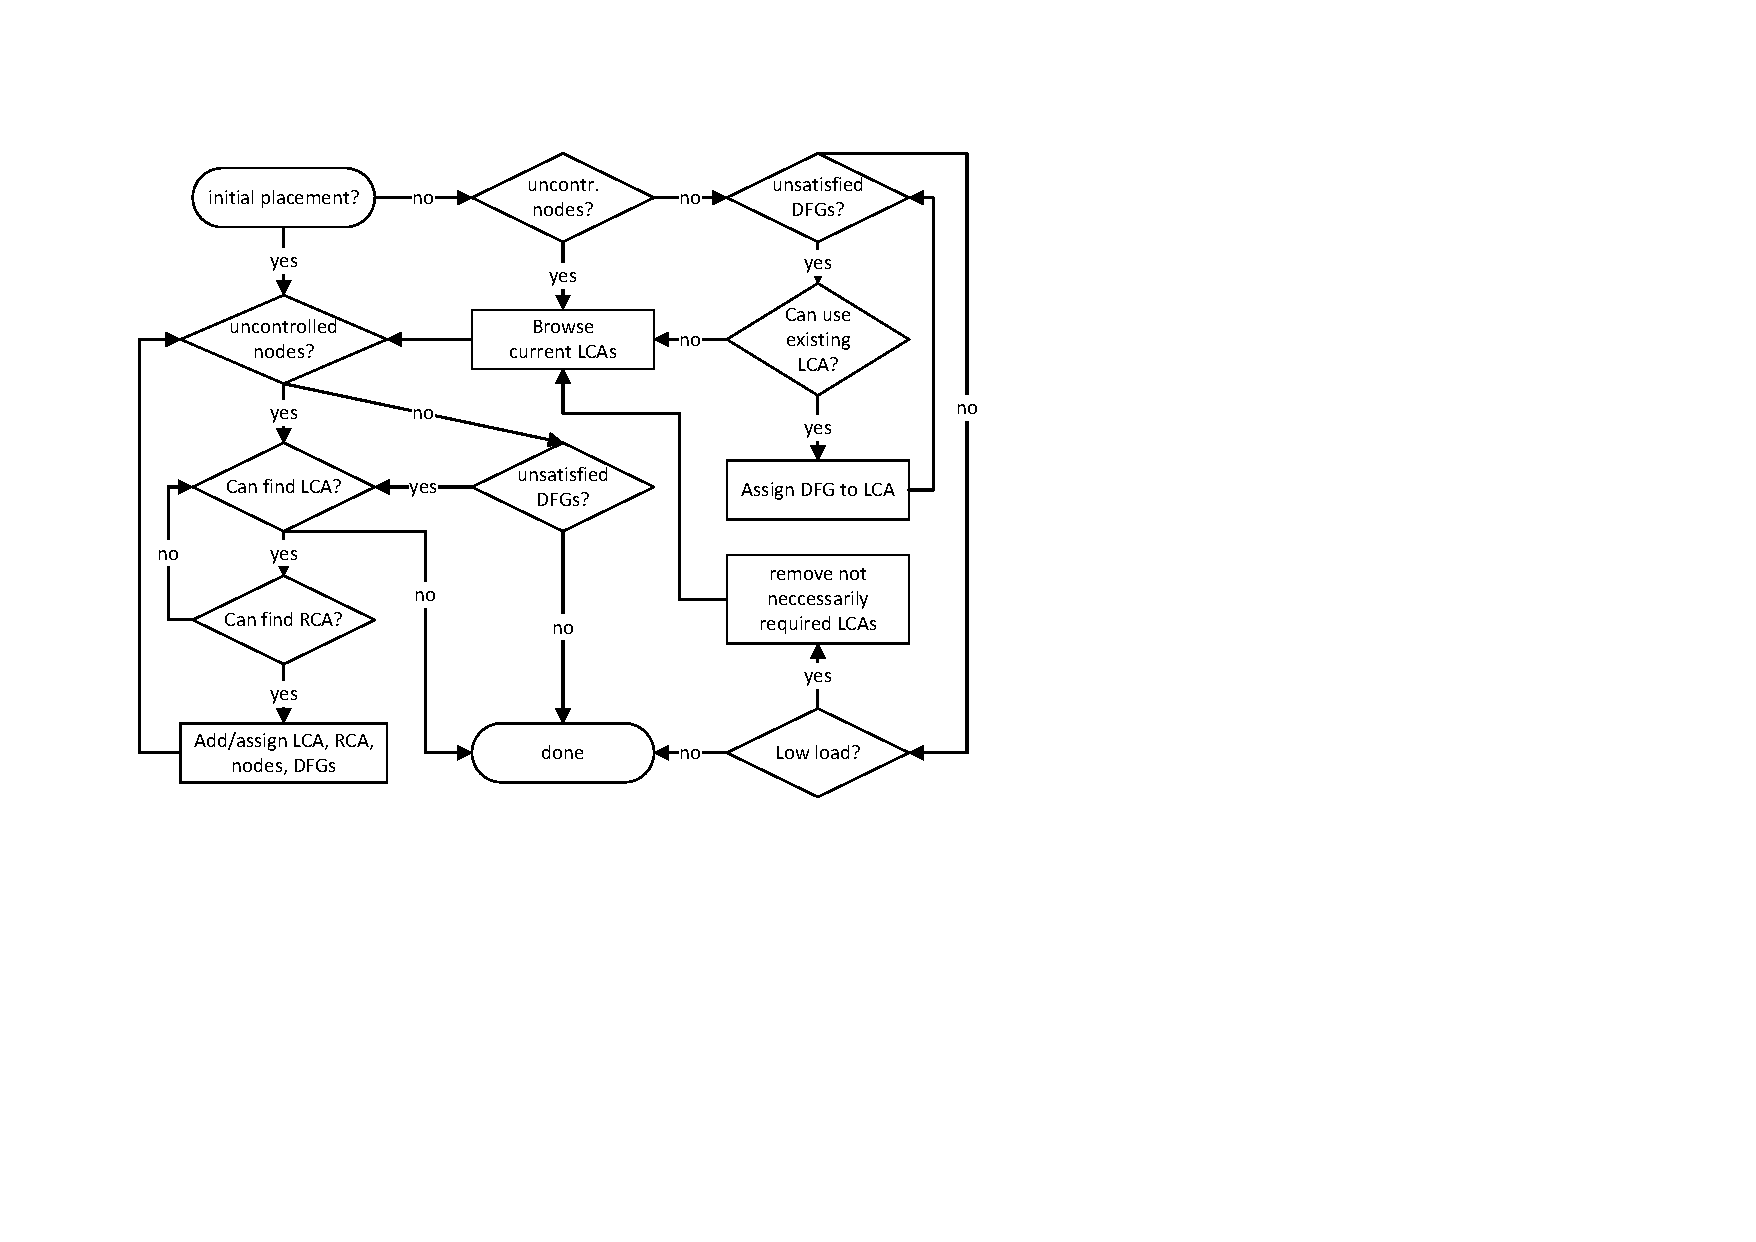
\includegraphics{flexfcpf-flowchart.pdf}}
	\caption{FlexFCAPF flow chart \cite{7343600}.}
	\label{fig:flexfcpfflow}
\end{center}
\end{figure}

\paragraph{Initial Controller Placement:}
FlexFCAPF works on a valid network; it is an internal state to specify that a network model is generated from an input topology description file successfully without any exception (see Section \ref{sec:emmod}). The algorithm first focus on node control, i.e., assign at least one LCA to each node of the network, then it changes focus to DFG satisfaction. The algorithm ends its execution if all DFGs are satisfied, if no more CAs are available, or if no new DFGs could be satisfied by adding an additional LCA, e.g., if all remaining DFGs cannot be satisfied with the network's remaining resources. At the end, the algorithm may clean up all LCA-to-node assignments that eventually did not serve any purpose, i.e., the LCA does not satisfy any data flow passing through the node and the node is assigned to more than one LCA.

To assign an LCA to a node, the algorithm has to determine the next potential CA to be added as LCA and get the appropriate LCA candidate based on different criteria. Then it makes sure an RCA is assigned to the selected candidate before adding it as LCA. This step is necessary to maintain the integrity of the two-layer CAs architecture (see Section \ref{sec:fcpf}). The candidate is confirmed as a new LCA if an RCA is found for it and can be assigned to the RCA.

To assign RCA to an LCA, the algorithm first try to get the nearest available RCA from the available RCAs. If no existing RCA can be assigned to an LCA candidate, a new RCA is added to the network considering all potential CAs that are not yet RCAs. FlexFCAPF tries to look for the most centralized potential RCA while looking for the first RCA in order to benefit all future RCA-to-LCA assignments. Otherwise, FlexFCAPF goes by the distance from RCA to the requesting LCA candidate. 

Once a node is assigned as an LCA, the algorithm also tries to assign DFGs to the new LCA ($v$). Depending on whether a network already has a complete control structure or not, it calculates the shortest paths from $v$ to all other nodes in the network. Later, the nodes are assigned to be controlled by the new LCA ($v$). During this process, the algorithm verifies that no model constraint is violated (see Section \ref{sec:ffps}).

When a node is assigned to LCA $v$, the algorithm updates the list of potential DFGs for $v$, i.e., the DFGs that are only passing through nodes that $v$ already controls and thus can be satisfied by $v$, provided there is sufficient resources available. Moreover, when $v$ is allowed to satisfy DFGs, FlexFCAPF successively try to assign the most demanding (in terms of requested processing capacity) DFG to $v$. The algorithm check all constraints before confirming a certain DFG is satisfied by $v$ (see Section \ref{sec:ffps}). In any case, the DFG is removed from the list of potential DFGs for $ v$, as it is either now satisfied by $v$ or it cannot be satisfied by $v$. 

Also, FlexFCAPF introduces a constraint, i.e., DFGs may only be satisfied by an LCA once it controls at least \textit{VCRatio} nodes that have previously been uncontrolled or if there are no more uncontrolled nodes in the network. Consider a situation where a network has many DFGs, and hence each LCA would have a lot of potential DFGs. After controlling only a few nodes, the LCAs may run out of resources by quickly satisfying many DFGs. In that case, a complete control structure would probably not be obtained. Hence, FlexFCAPF introduced that constraint to deal with such situation. At starting, VCRatio is initialized with a value $VCRatio = \frac{|V|}{|C|}$. 

\paragraph{Flexible Reassignment:}
There could be two scenarios which would trigger the network configuration change, i.e., reassignment of LCAs. One is Incoming DFGs and another is Low Load Situations. When a new DFG is added in the network, FlexFCAPF tries to assign it to one of the existing LCAs in the network. It first tries to assign the incoming DFG to the nearest possible LCA. If it fails to satisfy an incoming DFG, FlexFCAPF normally add a new LCA in the network and that will satisfy the new DFG.

Identifying a Low Load Situation is easy, but it is not trivial to remove an LCA while still satisfying all the DFGs in the network. FlexFCAPF continuously monitors the average LCA load in the network and if it stays below a threshold value, i.e., LCAloadlimit = 0.9 for 10 seconds or more, it removes unnecessary LCAs. This step will eventually move all the nodes and DFGs currently satisfied by the removed LCA to unsatisfied state again. Then, FlexFCAPF tries to assign those nodes and DFGs among all available LCAs. If FlexFCAPF could not reduce the number of LCAs from its earlier number, then, the low load correction is considered as failed and the LCAloadlimit is decreased by 0.05 for the next round.

\subsection{Modify Routing Table}\label{sec:mrt}
This is an important step for emulation. In emulation, real traffic is generated and that traffic has to follow a defined path (traffic generating node to its satisfying LCA) specified by FlexFCAPF algorithm. Every time FlexFCAPF algorithm is executed, there might be some new LCA introduced or may be some LCA removed. That would cause some nodes to be reassigned to new LCAs; this way, the path between the nodes and LCAs might change. To be in sync with the algorithm execution results, the emulation needs to modify the routing entries in the underlying network. The whole process is divided into three steps, i.e., populate network links, add routing entries, and delete routing entries.

\paragraph{Populate Network Links:}
The population of network links is a one-time job and this is done after starting the emulation network. Once the virtual network is created, all the connection between the network elements is retrieved by the Ryu SDN controller and saved it in an in-memory structure. This includes all the links' details and the interfaces belonging to each link. This is done by calling REST API provided by the controller over HTTP request. This information is necessary because the routing entries in the underlying network have to be in sync with FlexFCAPF defined path. That is why the emulation prepares each forwarding entry which needs to be added in the underlying network elements. The emulation uses this information while preparing the forwarding entries for the underlying network. Listing \ref{lst:pnli} shows the code implementation of the same.

\begin{lstlisting}[caption={Populate network links implementation},label={lst:pnli},language=Python,tabsize=2,basicstyle=\footnotesize,breaklines=true, showspaces=false,showstringspaces=false,showtabs=false,frame=single]
def populateNetworkLinks(self):
	urlpath = "http://127.0.0.1:8080/fcapfnetworkcontroller/topology/links"
	resp = requests.get(urlpath)
	self.Links = resp.json()
\end{lstlisting}

\paragraph{Add Routing Entries:}
This step has to be executed every time FlexFCAPF algorithm is executed. The method \textit{modifyRoutingTable} (see Listing \ref{lst:mrti}) is responsible for that purpose. When this method is called for the first time, it loops through all the path between the nodes and it satisfies the LCA. It prepares an entry request for each link in the path by calling the method \textit{addRoutingPath}. Before that, it checks if the routing path between them already exists or not by calling \textit{checkRoutingPath} method.

\begin{lstlisting}[caption={Modify routing table implementation},label={lst:mrti},language=Python,tabsize=2,basicstyle=\footnotesize,breaklines=true, showspaces=false,showstringspaces=false,showtabs=false,frame=single]
def modifyRoutingTable(self):
	for n in self.cn.G.node:
		node = self.cn.G.node[n]
		pathToLCA = node['pathtoLCA']
		for clc, path in pathToLCA.items():
			src = clc
			dst = n
			foundPath = self.checkRoutingPath(src, dst, path)
			if foundPath == False:
				self.addRoutingPath(src, dst, path)
	self.requestAddRoutingEntries()
	self.clearObsoleteRoutingPaths()
	self.requestDeleteRoutingEntries()
\end{lstlisting}
The \textit{checkRoutingPath} (see Listing \ref{lst:crpi}) checks it by comparing the input path with its earlier saved list of the path in an in-memory structure \textit{RoutingPaths}. If the path is not present in the in-memory structure \textit{RoutingPaths}, it adds the path in that structure. It also prepares a temporary list of all current paths \textit{CurrentRoutingPaths}. By adding the non-existing path in the network, the emulation gets two benefits. First, it is only adding the difference path but not the complete path, thus, saving processing time for the controller and the underlying network elements. Another benefit is, it is not disturbing the traffic which is running in the network at that moment.

\begin{lstlisting}[caption={Check routing path implementation},label={lst:crpi},language=Python,tabsize=2,basicstyle=\footnotesize,breaklines=true, showspaces=false,showstringspaces=false,showtabs=false,frame=single]
def checkRoutingPath(self, src, dst, path):
	key = (src, dst, path)
	self.CurrentRoutingPaths.append(key)
	foundPath = key in self.RoutingPaths
	if foundPath == False:
		self.RoutingPaths.append(key)
	return foundPath
\end{lstlisting}

The \textit{addRoutingPath} method prepares the flow table entry information with the help of the real links information which is saved earlier and add those entries to a list \textit{JsonEntries} for creating forwarding entry in the network. For each link in a path, a total of four entries will be created, i.e., one for inward traffic and one for outward traffic; and for each way traffic, two types of entries is created, one for ARP packet and another for IP packet. Since it is a lengthy repetitive code, the code implementation is not presented here for this method. One important point to remember is that a standard was followed for assigning the IP address to host and MAC address to the switch while creating the network. That information is necessary to create the forwarding entries in the network elements. Because the forwarding entry's match conditions are prepared based on the source IP address, destination IP address and the MAC address are necessary for specifying where to add the entry.

The \textit{requestAddRoutingEntries} (see Listing \ref{lst:rarei}) method takes all the \textit{JsonEntries}, the newly prepared flow table entry list, and calls the \textit{addflows} REST API provided by the controller to actually create forwarding rules in the underlying network elements.
\begin{lstlisting}[caption={Request add routing entries implementation},label={lst:rarei},language=Python,tabsize=2,basicstyle=\footnotesize,breaklines=true, showspaces=false,showstringspaces=false,showtabs=false,frame=single]
def requestAddRoutingEntries(self):
	url = "http://127.0.0.1:8080/fcapfnetworkcontroller/flowtable/addflows"
	data = json.dumps(self.JsonEntries)
	resp = requests.put(url, data=data)
	if resp.status_code != 200:
		print "Something is wrong adding Routing entries, check controller log!!"
	del self.JsonEntries
	self.JsonEntries = []
\end{lstlisting}

\paragraph{Delete Routing Entries:}
Similar to the add routing entries, the delete routing entries also have two steps; first, it cleans up all the obsolete entries from the in-memory routing path, i.e., \textit{RoutingPaths}. The method \textit{clearObsolateRoutingPaths} (see Listing \ref{lst:corei}) is used to clean up all the obsolete paths which are present in the in-memory \textit{RoutingPaths}. This is done by comparing two list of routing paths, i.e., \textit{RoutingPaths} and \textit{CurrentRoutingPaths}. It is important to notice that \textit{CurrentRoutingPaths} is prepared in the method \textit{checkRoutingPath} during add routing entries. The \textit{CurrentRoutingPaths} contains only those entries which are provided by last FlexFCAPF run and \textit{RoutingPaths} contains all the entries which are already added in the underlying network. The path provided by the latest run only should exist in the underlying network, others have to be removed. For doing that, the \textit{clearObsoleteRoutingPaths} calls \textit{deleteRoutingPath} method to prepare a list of \textit{JsonEntries} which needs to be removed from the underlying network. Finally, \textit{requestDeleteRoutingEntries} is used to remove forwarding rules from the network elements. The method \textit{requestDeleteRoutingEntries} acts similarly like \textit{requestAddRoutingEntries}, i.e., calls the \textit{delflows} REST API provided by the controller. The method \textit{deleteRoutingPath} also works similar to \textit{addRoutingPath}.

\begin{lstlisting}[caption={Clear obsolete routing entries implementation},label={lst:corei},language=Python,tabsize=2,basicstyle=\footnotesize,breaklines=true, showspaces=false,showstringspaces=false,showtabs=false,frame=single]
def clearObsoleteRoutingPaths(self):
	entries = copy.deepcopy(self.RoutingPaths)
	for entry in entries:
		(src, dst, path) = entry
		if entry not in self.CurrentRoutingPaths:
			self.deleteRoutingPath(src, dst, path)
			self.RoutingPaths.remove(entry)
	del entries
	del self.CurrentRoutingPaths
	self.CurrentRoutingPaths = []
\end{lstlisting}
It is important to note that the REST API calls are made two times: once for adding and once for deleting flow entries. This is done to reduce parsing efforts at the controller. If the controller receives both types of request at the same time, it has to check each entry for the type of request. By separating addition and deletion in two calls, the logical implementation is also kept separate.

\subsection{DFG Processing}\label{sec:tmfg}
Implementing real data processing is not a feasible option in the emulation environment due to resource constraints, i.e., it needs a hardware with more CPU power and memory. I developed an alternative way achieve data processing capability in the CA. Ideally, there are three steps necessary to have a real data processing in the testbed. These steps are capturing the packet, executing some processing logic on the packet, and sending the packet back to the source. The concept of data processing here is, instead of doing some real processing on the captured packet and resending it back to the source, just delay the packet in the CA before sending. The idea is actual processing (i.e., run some processing logic) would take some time, e.g., $\Delta t$; instead of running processing logic, simply delay the packet in CA for that $\Delta t$ time and then send the packet back to the source. This way, by introducing a waiting time for each packet in the CA, the processing capability is achieved. The waiting time for each packet of different DFG would not be the same; each DFG would need a different processing time, i.e., delay. To deal with this problem, I introduced a concept of adding an identifier to the packet. FlexFCAPF gives processing time (delay) required for processing a packet of a particular DFG. Now, I have the packet identifier and the delay needs to be applied on the packet. Using this information, I am configuring filters and queues in the CAs. This is done using Linux networking tools \textit{tc} and \textit{netem} (see Section \ref{sec:tan}).

\begin{figure}[H]
	\begin{center}
		\resizebox{\textwidth}{!}
		{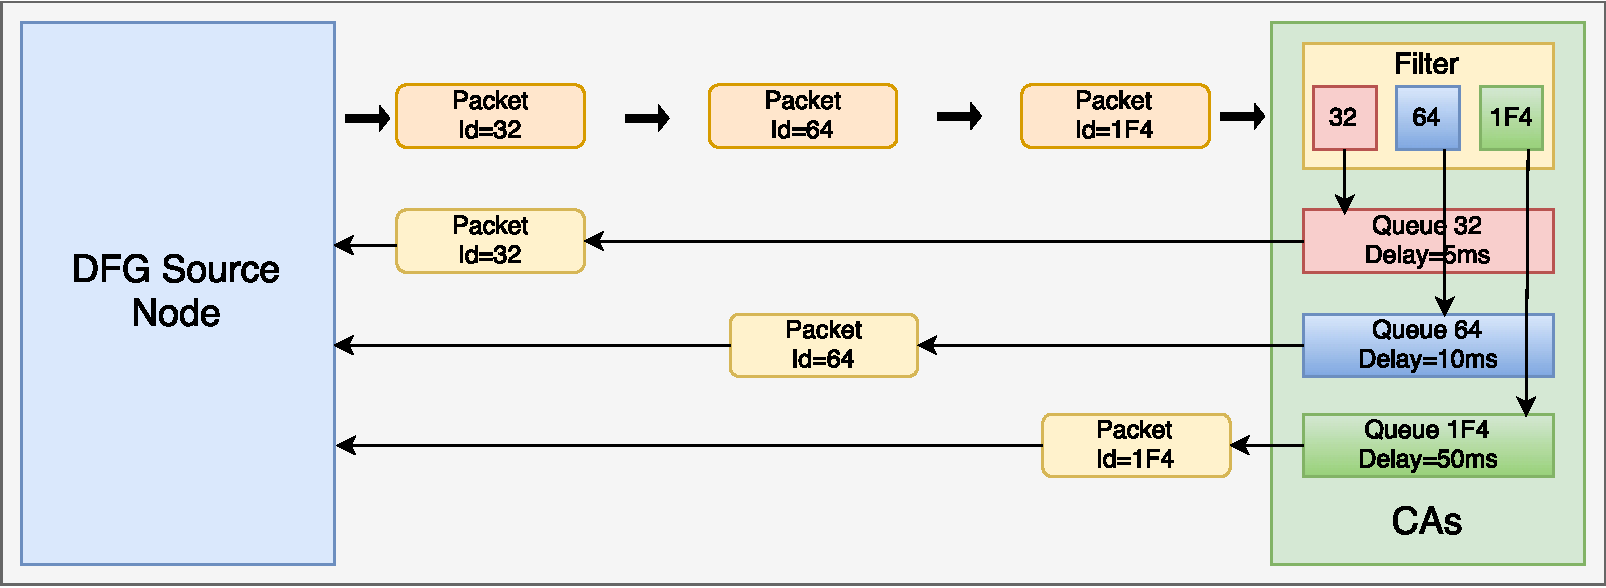
\includegraphics{dataprocessing.pdf}}
		\caption{Data processing overview.}
		\label{fig:dataproc}
	\end{center}
\end{figure}

Figure \ref{fig:dataproc} shows an overview of the data processing implementation in the testbed. The traffic generator in the DFG source node adds an identifier to each packet it generates (see Section \ref{sec:tragen}). Then, the packet travels through the network and reaches the satisfying LCA, and in turn, the LCA sends the same packet back to the source. When the packet goes out of the LCA, the data processing delay is applied on the packet. Before starting traffic generation, a delay configuration needs to be done in the satisfying LCA. The traffic control configuration is done by executing a small script shown in listing \ref{lst:cdi} on the LCA.

\begin{lstlisting}[caption={Configure delay implementation},label={lst:cdi},language=bash,tabsize=2,basicstyle=\footnotesize,breaklines=true, showspaces=false,showstringspaces=false,showtabs=false,frame=single]
if tc qdisc show dev "$interface" | grep "qdisc htb $r_handle:" > /dev/null; then
	qdpresent=true
else
	qdpresent=false
fi
if [ $qdpresent != true ]; then
	if not ( tc qdisc add dev "$interface" root handle $r_handle: htb;) then
		exit 1
	fi
fi
if not (tc class add dev "$interface" parent $r_handle: classid $r_handle:$n_handle htb rate 2500Mbit;) then
	exit 1
fi
if not (tc qdisc add dev "$interface" parent $r_handle:$n_handle handle $n_handle: netem delay ${delay}ms;) then
	exit 1
if not (tc filter add dev "$interface" parent $r_handle:0 protocol ip prio 1 u32 classid 1:$n_handle match u32 $flowid 0xffffffff at 28;) then
	exit 1
fi
\end{lstlisting}

To configure the delay for each specific Id of the packet, three traffic control objects (a \textit{class}, a \textit{qdisc}, and a \textit{filter}) need to be configured in the output network interface of the LCA host. The queue (i.e., \textit{qdisc}) is associated with the \textit{class} and the delay value (which is applied to the outgoing packet) is assigned to the queue, and all these classes are associated to a root queue. The \textit{filter} is directly associated with the root queue and it has an additional association with the class. The \textit{filter} has a match condition and the match condition is set as the packet identifier. Therefore, whenever a packet goes out of the LCA, the \textit{filter} matches the packet data field (the field where the identifier is saved), and if a match is found, that packet will be handled by the respective class associated with the filter. Eventually, the class will put the packet in the queue which is attached to the class. The packet will wait in the queue for the configured delay specified for the queue, then the packet will go out of the LCA after waiting for the delay. It is important to remember here that the LCA will return the same packet back, no modification is done in the packet inside the LCA. So the packet will contain the identifier which is set by the generator. 

Listing \ref{lst:tcoce} shows a sample traffic control object's configuration setup. This is done by the shell script in Listing \ref{lst:cdi}, the script takes five input parameters: the interface, the root key, a child key (usually the packet identifier), the delay and the match condition (this is also the packet identifier but HEX value). First, the script checks for the root qdisc if not present then add the root qdisc in the interface with handle = ``rootkey:". Then it adds a class with classid = ``rootkey:childkey" and a child qdisc with handle = ``childkey:", parent = ``rootkey:childkey" and netem delay = ``delay value" in the interface. Finally, it adds a filter in the interface with parent = ``rootkey:0", classid = ``1:childkey" and match condition = ``match condition value"

\begin{lstlisting}[caption={Traffic Conroller object's configuration example},label={lst:tcoce},language=bash,tabsize=2,basicstyle=\footnotesize,breaklines=true,showspaces=false,showstringspaces=false,showtabs=false,frame=single]
$h10 tc class show dev h10-eth0
class htb 1:100 root leaf 100: prio 0 rate 2500Mbit ceil 2500Mbit burst 1250b cburst 1250b
class htb 1:500 root leaf 500: prio 0 rate 2500Mbit ceil 2500Mbit burst 1250b cburst 1250b

$h10 tc qdisc show dev h10-eth0
qdisc htb 1: root refcnt 2 r2q 10 default 0 direct_packets_stat 17188 direct_qlen 1000
qdisc netem 100: parent 1:100 limit 1000 delay 10.0ms
qdisc netem 500: parent 1:500 limit 1000 delay 50.0ms

$h10 tc filter show dev h10-eth0
filter parent 1: protocol ip pref 1 u32
filter parent 1: protocol ip pref 1 u32 fh 800: ht divisor 1
filter parent 1: protocol ip pref 1 u32 fh 800::800 order 2048 key ht 800 bkt 0 flowid 1:100 match 00000064/ffffffff at 28
filter parent 1: protocol ip pref 1 u32 fh 800::801 order 2049 key ht 800 bkt 0 flowid 1:500 match 000001f4/ffffffff at 28
\end{lstlisting}

Figure \ref{fig:tcobjhier} shows an example of Traffic Control object's hierarchy of a network interface. Each interface has a root queue (qdisc), which is the default. For packet identifier ``00000064", an HTB class with id ``1:100", a netem qdisc with id ``100:", and a filter with id ``800::801" associated to class id ``1:100" are configured. The qdisc with id ``100:" have a delay of 10.0ms and the filter with id ``800::801" have a match condition ``"00000064/ffffffff" configured. This means when a packet with identifier ``00000064" goes out of this interface, it will be delayed by 10.0ms. Similarly, for packet identifier ``000001f4", the same set of objects are configured.

\begin{figure}[H]
	\begin{center}
		\resizebox{\textwidth}{!}
		{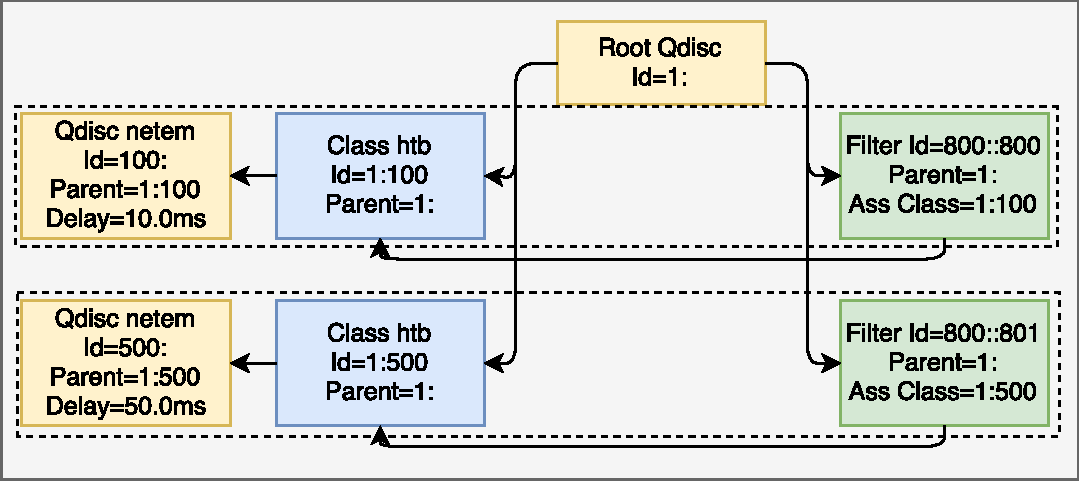
\includegraphics{tcobjectshierarchy.pdf}}
		\caption{Traffic Control object's hierarchy.}
		\label{fig:tcobjhier}
	\end{center}
\end{figure}

\subsection{Traffic Generation}\label{sec:tragen}
Once a DFG is satisfied by FlexFCAPF, the emulator has to start the traffic generation for the same. It is done by running an \textit{iperf} client in the source node to generate real UDP network traffic. I am generating UDP packet to use the iperf functionality of generating controlled traffic. In UDP mode only iperf support specifying the bandwidth parameter (-b) to control the data rate of the generated traffic. The method \textit{generateTrafficForSingleFlow} (see Listing \ref{lst:tgi}) is doing this job; it retrieves the list of source nodes through which the DFG entered the network, i.e., where the \textit{iperf} client instance will be launched, and the satisfying LCA, i.e., the sink of the DFG or the processing CA. Before starting the \textit{iperf} instance on the source node, the configuration of the data processing is made in the satisfying LCA (see Section \ref{sec:tmfg}). A bucket\_id (explained in next paragraph) is assigned to each DFG which I call DFG identifier, and the data processing configuration will be done only if the configuration for the same DFG identifier was not made already in the LCA. The method \textit{checkBucketInLCA} internally maintains a list of key (combination of the LCA and the DFG identifier) to check that the same configuration has not been executed multiple times. This saves some processing time of the emulation and improves performance.

\begin{lstlisting}[caption={Traffic generation implementation},label={lst:tgi},language=python,tabsize=2,basicstyle=\footnotesize,breaklines=true,showspaces=false,showstringspaces=false,showtabs=false,frame=single]
def generateTrafficForSingleFlow(self, fid):
	flow = self.cn.fdata[fid]
	if flow['isSat'] == True and flow['isGen'] == False:
		self.getHostForFlow(fid)
		dur, bw = flow['duration'], flow['b_flow'] / 2
		delay = self.cn.fdata[fid]['p_flow'] / self.cn.G.node[flow['CLC']]['ProcFlow'][fid] * 1000
		bucket_id = int(round(delay * 10))
		hName = "h" + str(flow['CLC'])
		clcObj = self.TestbedNetwork.get(hName) if self.emulator == "Mininet" else self.TestbedNetwork.get_node(hName)
		clcIP = Tools.makeIP(flow['CLC'] + 1)
		for hObj in self.hObjs:
			(n,obj)=hObj
			id = bucket_id + n * 1000
			bucket_id = bucket_id + n * 65536
			hexFid = "0x%0.8x" % bucket_id
			if False == self.checkBucketInCLC(flow['CLC'], bucket_id):
				clcObj.cmd(g_conf_script_path + " add " + hName + "-eth0 1 " + str(id) + " " + str(delay) + " " + hexFid)
			obj.cmd(g_iperf_path + " -u -c " + clcIP + " -f b -b " + str(bw) + " -t " + str(dur) + " -k " + str(bucket_id) + " > /tmp/iperf_client_" + str(fid) + "_" + str(bw) + "_" + str(dur) + "_" + str(obj.name) + "_to_" + str(hName) + ".log &")
			self.cn.fdata[fid]['genstime'] = time.time()
			self.cn.fdata[fid]['isGen'] = True
			self.TotalSatisfied.append(fid)
			if fid in self.TotalUnsatisfied:
				self.TotalUnsatisfied.remove(fid)
	elif flow['isSat'] == False:
		self.TotalUnsatisfied.append(fid)
	else:
		pass  # do nothing
\end{lstlisting}

While starting the \textit{iperf} instance, it takes some parameters as follows (see Listing \ref{lst:iece}):
\begin{itemize}
	\item u - to specify it as an UDP client.
\item c - the destination of the traffic, i.e., the satisfying LCA.
\item f - to specify the iperf output report format; here it is b for Bits.
\item b - to specify the data rate of the traffic flow. There is one point to take note while setting the data rate value. In FlexFCAPF algorithm, a DFG is assigned a total data rate for both way communication, but while generating real traffic, it has to be half since half is for uploading and another half for downloading traffic.
\item t - to specify the runtime of the traffic generation.
\item k - to specify the identifier to be added to the generated packet.
\end{itemize}

Generally, \textit{iperf} does not take any parameter to include user-provided information in the packet. Since it is an important requirement for emulation, I modified the \textit{iperf} code to have an additional parameter (k) to pass user information and include that information in the packet. It is important to know that the identifier was converted into HEX value and used it while configuring the filter. It is done to match the traffic control's filter object match condition. The filter can compare HEX value and the maximum size of the HEX value could be of 4-byte length. For this reason, the identifier passed in the \textit{iperf} with `-k' will be converted to HEX and then the HEX value will be added as the first 4-byte data field of the generated packet. After starting the \textit{iperf} instance, the traffic generation start time is saved for future reference and marked the DFG, saying that the traffic generation has been done already.

\begin{lstlisting}[caption={Iperf instance command example},label={lst:iece},language=bash,tabsize=2,basicstyle=\footnotesize,breaklines=true,showspaces=false,showstringspaces=false,showtabs=false,frame=single]
iperf -u -c 10.0.0.24 -f b -b 1248799.83444 -t 50.4681735561 -k 100
iperf -u -c 10.0.0.11 -f b -b 5548016.7046 -t 46.372407258 -k 500
\end{lstlisting}

Initially, I was using the DFG Id provided by the DFG generator of the emulator as the identifier of the packet. The DFG Id is unique for each DFG in the emulation run. There are thousands of DFG in a run, and for this reason, I have to configure thousands of traffic control objects in the LCA interface. However, it has multiple disadvantages. First, it takes lot of processing time to configure the objects in the LCA, and second, it takes a lot of resources to have all the traffic objects available in the system; finally, when a packet pass through the interface, the interface has to make thousands of comparison before it gets the matched filter. To deal with this problem, I introduced a concept of the bucket. DFGs are grouped into buckets based on two parameters: one is the delay of the DFG another is the DFG source and then assigned a bucket id. A bucket is created for each DFG source and for each delay interval of 0.1 ms. I have a total of 4 bytes to prepare bucket id, I am using 2 bytes to specify DFG source node id and another 2 bytes for specifying the delay interval value. For example, a DFG source node id is 8 and the delay is 5 ms, 2 bytes for node id 8 = 0x0008 and 2 byte for $5\times10 = 50$ = 0x0032, so the final bucket id = 0x00080032. The bucket id is used as the identifier of the packet to be generated for the DFG. I also call the bucket id as DFG identifier.

By combining the DFG source node and the delay, I got two benefits. First, I reduced the number of traffic control object for only 0.1 interval of delay, i.e., for the delay range of 1.0ms to 1.9ms there is 10 bucket (10 to 19) and it is important to know that the traffic control configuration for a delay is set only if there is a DFG added with that specific delay. Second, I could maintain a level of uniqueness by adding the source node id, which means two packets with the same interval from different source node will be handled separately.

\subsection{Stop Traffic Generation}
FlexFCAPF may execute the low load scenario and might reassign some DFG in that process. If a DFG is reassigned, then the DFG might be reassigned to a new LCA. In that case, first, the real traffic generation needs to be stopped for that specific DFG and restarting the traffic generation for that might be with different \textit{iperf} parameter altogether. This is done by calling the method \textit{stopTrafficGenerationForSingleFlow} (see Listing \ref{lst:stgi}). It checks whether the DFG ran for a specified duration; if not, then it stops the \textit{iperf} instance in the source node of the DFG and modify the duration of the DFG with the remaining duration yet to be run. This way, when the DFG is satisfied, it will run for the remaining duration only the next time. Traffic generation will be restarted when the DFG will be satisfied the usual way.

\begin{lstlisting}[caption={Stop traffic generation implementation},label={lst:stgi},language=python,tabsize=2,basicstyle=\footnotesize,breaklines=true,showspaces=false,showstringspaces=false,showtabs=false,frame=single]
def stopTrafficGenerationForSingleFlow(self, fid):
	flow = self.cn.fdata[fid]
	currTime = time.time()
	# giving 0.01 sec extra time assuming the processing time of to start the ipref
	if (flow['duration'] > currTime - flow['genstime'] + 0.01) and flow['isSat'] == True and flow['isGen'] == True:
		self.getHostForFlow(fid)
		lcaIP = Tools.makeIP(flow['LCA'] + 1)
 		dur, bw = flow['duration'], flow['b_flow'] / 2
		searchStr = "iperf -u -c " + lcaIP + " -f b -b " + str(bw) + " -t " + str(dur)
		for hObj in self.hObjs:
			hObj.cmd("ps -eaf|grep \"" + searchStr + "\"|awk \'{print \"kill -9 \" $2}\'|sh")
		self.cn.fdata[fid]['duration'] = flow['duration'] - (currTime - flow['genstime'])
		self.cn.fdata[fid]['isGen'] = False
		self.TotalFlowStopped.append(fid)
		if fid in self.TotalSatisfied:
			self.TotalSatisfied.remove(fid)
\end{lstlisting}

\section{Emulation Execution} \label{sec:emuexec}
I have described the different modules and its implementation in details in the previous sections. Here, I will describe the main flow of the emulation testbed execution. Figure \ref{fig:emulationflow} illustrates the overall workflow of the emulation execution in a flow chart.
\begin{figure}[tb]
\begin{center}
	\resizebox{\textwidth}{!}
	{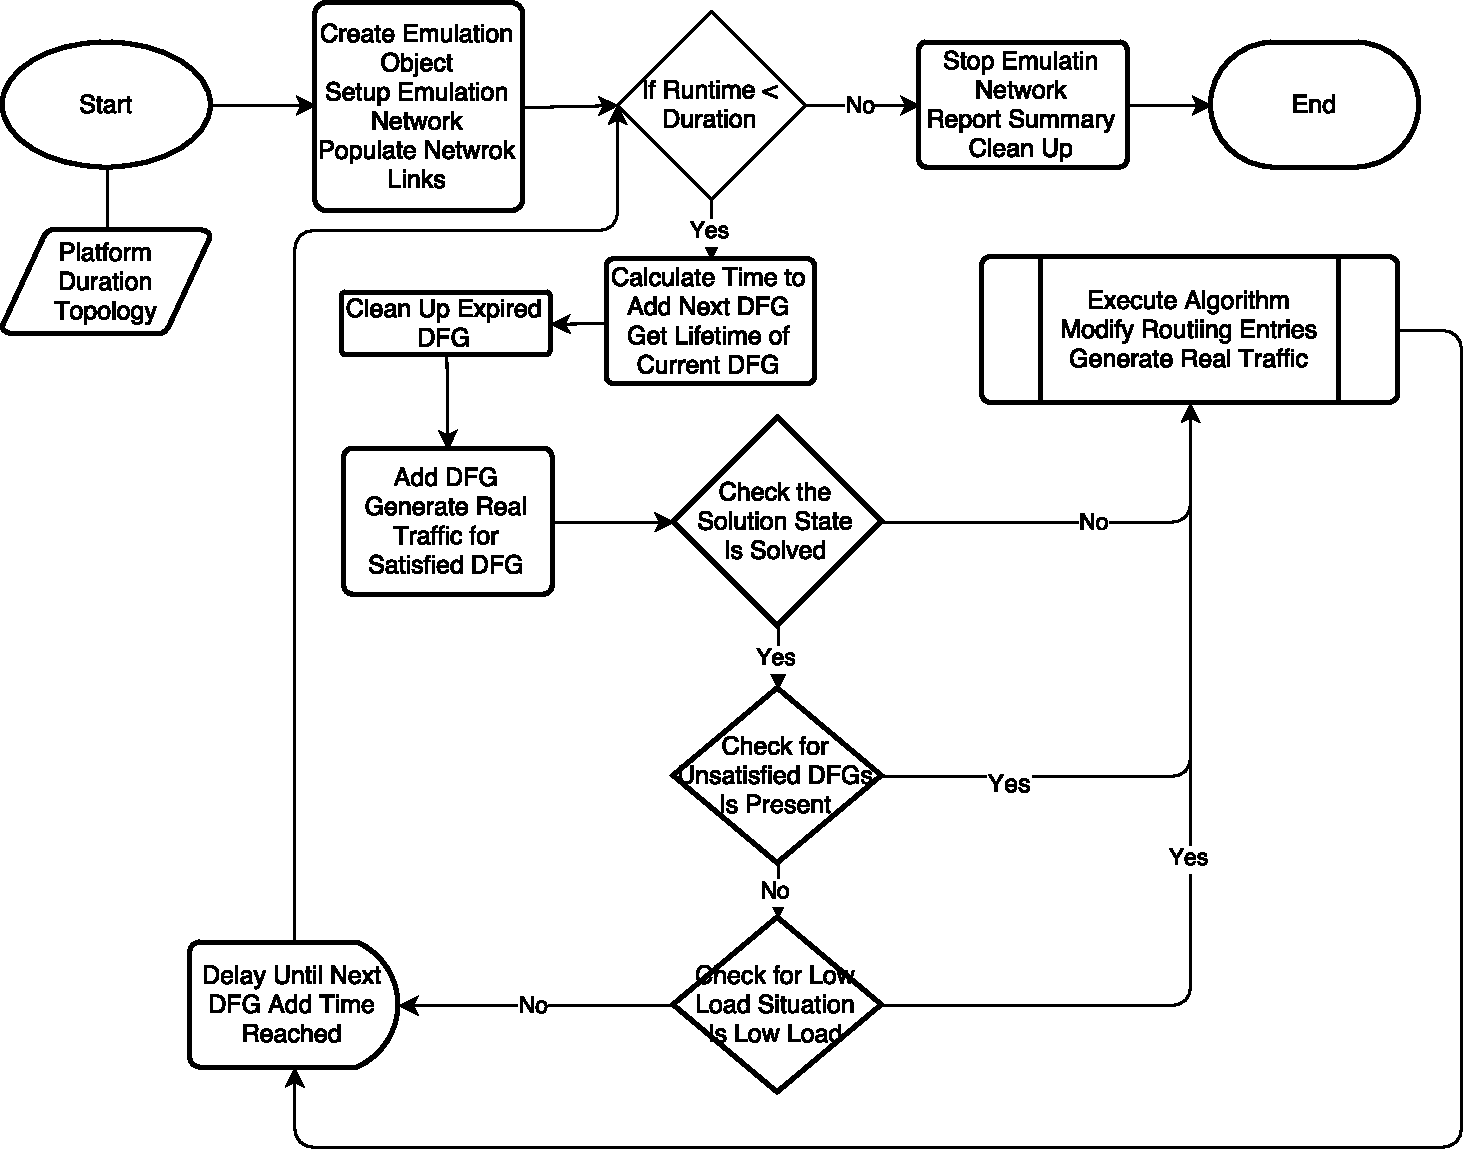
\includegraphics{emulation-flowchart.pdf}}
	\caption{Emulation flow chart.}
	\label{fig:emulationflow}
\end{center}
\end{figure}

The emulation starts with three input parameters, the emulation platform (Mininet or MaxiNet), the duration (how long the emulation will be executed) and the testbed topology description file. First, it creates an emulation object which is basically an object of class \textit{CPFlex}, which prepare the network model reading the topology description file. Then, it set up the network by calling the method \textit{setupEmulationNetwork} (see Section \ref{sec:setnet}); it uses the network model and set up the real network testbed based on specified emulation platform. The method \textit{populateNetworkLinks} (see Section \ref{sec:mrt}) is used to populate the network links information. After which, it starts the loop of the emulation for the specified amount of time the emulation needs to run. Inside the loop, it first calculates a period of time to add the next DFG in the system. I call that period of time $\Delta t$, in that $\Delta t$ the emulation executes following steps:
\begin{itemize}
	\item It handles the blacklisted flows (if any) and remove all the flows which have already expired. Blacklisted flows are those which are on the system but could not be satisfied with the available resources. Therefore, they are blacklisted for a short period of time so that the algorithm does not fall into a loop of repeatedly trying to satisfy them unsuccessfully.
	\item It adds a new DFG in the system and starts real traffic generation for the same. It is important to remember that FlexFCAPF tries to satisfy the DFG when it is added to the system.
	\item It checks if there are any unsatisfied, non-blacklisted DFGs in the network and if there are still unsatisfied DFGs, the emulation set a boolean for executing FlexFCAPF algorithm for the reason of ``Unsatisfied flow in the system".
	\item It moves on and checks for low load situation, if there is no unsatisfied, non-blacklisted DFGs. For low load situation, it tries to remove the lowest loaded LCA from the system and set a boolean to execute FlexFCAPF algorithm with the reason of ``Low Load Situation" to reassign the DFGs and nodes which were assigned to the removed LCA.
	\item If the boolean for executing FlexFCAPF is set, the emulation execute the algorithm. Every time FlexFCAPF algorithm has been executed, there might be a change in the node to LCA assignment, therefore the emulation modifies the routing entries in the underlying network to accommodate that changes via REST API call to the SDN controller. It also configures traffic control objects in the LCAs to introduce delay in the interfaces and starts iperf to generate traffic for all the newly satisfied flows due to resignment.
\end{itemize}
If the emulation could finish all the steps before the $\Delta t$ system time then it sleeps for the remaining time, otherwise, it goes for next iteration of executing above steps. Finally, when the specified emulation duration is reached, it ends the loop, stop the network and do the cleanup.
         % Chapter 3
% chap4.tex (Evaluation)
\newpage
\thispagestyle{empty}
\mbox{}


\chapter{Evaluation}\label{EVAL-CHAP}
Many test scenarios have been executed during the setup of the testbed, variety of issues were found in the setup process (see Chapter \ref{IMPL-CHAP}). Therefore, approaches were changed and the code has been modified based on the outcome. In this chapter, I describe only those scenarios which gave the best results considering the resource limitation of the emulation testbed. In Section \ref{sec:tbcfg}, I give the details about the basic configuration of the testbed. In Section \ref{sec:expscn}, I talk about the experiment scenario I executed for evaluation and analysis. In Section \ref{sec:poct}, I describe the proof of concept test scenario and their results.. In Section \ref{sec:rgra}, I talk about report generation and the analysis of the execution results. Finally in Section \ref{sec:cws}, I compare the results of both simulation and emulation environment.


\section{Testbed Configuration}\label{sec:tbcfg}
Emulation scenario executed in both Mininet and MaxiNet platforms. Execution scenario of Mininet platform is executed in one single machine with 4 core Intel i5-3320M CPU running at 2.60GHz having 8GB RAM. The hardware details of MaxiNet platform is specified in section \ref{sec:infra}.

\subsection{Topology}
I used mesh topology for execution of all the evaluation scenarios in Mininet and used both mesh and ring topology for MaxiNet scenarios. While setting up the network, the model specified in \cite{7343600} was used and its overview as explained in that paper is described here. All the nodes are placed on a regular grid with a mean inter-node distance of $\bar{s} = 1000m$ and they are shifted in both $x$ and $y$ directions by normally distributed random variables with zero mean and a standard deviation of $\frac{\bar{s}}{8}$. In the mesh topology, a link between two nodes is created if the distance between them is less or equal to $1.5 \times \bar{s}$. A maximum link bandwidth of 500Mb is set for mesh topology link. The model for ring topology used here is a back-haul modeled similarly to the metro ring \cite{tbiermann}. In the ring topology, the ring center and the radius is calculated based on $\bar{s}$ and $\sqrt{number\ of\ nodes}$. Links are created between the nodes which are on the circumference of the ring with link bandwidth of 750Mb and other nodes are connected to its nearest neighbor node in the ring with the link of 500Mb bandwidth. Out of all nodes, some nodes are capable of running CAs; a probability value of 0.6 is used to decide if a node is a potential candidate for a CA or not. A maximum processing capacity of 40 GFLOPS is set for all nodes capable of being CA.

It is important to know that while creating the emulation network, those limitations are not introduced. That means all the Mininet/MaxiNet nodes (switches, hosts) are sharing the complete processing capacity of the hardware it is running on. Similarly, no bandwidth limitation is introduced on the link created between the Mininet/MaxiNet nodes. FlexFCAPF knows which node has how much processing capacity and which link has how much bandwidth; when the algorithm sees an LCA does not have enough processing capacity to satisfy a DFG, it will not assign any DFG to that LCA. Therefore, it is not necessary to emulate those limitations in the emulation network. Moreover, for introducing bandwidth capacity limitation, some traffic control objects need to be created and for limiting CPU processing capacity, process group need to be created for each node. I did not see any benefits of doing that and furthermore, it will load the testbed by eating some processing capacity of the hardware.
 
\subsection{Traffic Model}
Researchers usually use the Poisson process for traffic generation of circuit-switched data as well as packet data. The number of incoming packets or calls per time unit follows the Poisson distribution. The length or the duration of each phone call is typically modeled as an exponential distribution. Emulation also uses similar traffic generation model mentioned in this paper \cite{7343600} while simulation uses a non-stationary Poisson process with $\lambda = |V| \times loadlevel(t)$ and the thinning method \cite{Law:1999:SMA:554952} for DFG generation. A daily load level curve (see Figure \ref{fig:24loadlevel}) is prepared based on the cellular data traffic characteristics explained in \cite{Zhang:2012:UCC:2342468.2342472}. In emulation, the same model for traffic generation is used with a modified $\lambda = |V| \times loadlevel(t, scaling)$. Load level factor $scaling$ is added to set the scaling of the load level; this is done to control load level for different scenario and due to the hardware resource limitation in the emulation environment. The duration of the DFG is set by an exponential variable with parameter $0.02$ which means the expected average duration is 50 seconds and that an approximated number of DFGs in the network at any time $t$ is $50 \times |V| \times loadlevel(t, scaling)$. The execution scenario is divided into two sections based on flow types. One is the generic \cite{7343600} scenario and another is CoMP \cite{MArasha} scenario. Attributes specified in Table \ref {tab:gendfgtype} for generic scenario and in Table \ref {tab:compdfgtype} for CoMP scenario are used while generating DFGs.

\begin{table}[h!]
	\centering
	\caption{Generic data flow group types \cite{7343600}}
	\label{tab:gendfgtype}
	\begin{tabular}{c | c | c | c}
		\hline
		Type & Probability & $b_{flow}$ & $l_{flow}$\\
		\hline
		voice & 0.5 & 500 Kbits/s & 5 ms\\
		video & 0.4 & 1 to 4 Mbits/s & 10 ms\\
		data & 0.1 & 1 to 20 Mbits/s & 50 ms\\
		\hline
	\end{tabular}
\end{table}

\begin{table}[h!]
	\centering
	\caption{CoMP data flow group types \cite{MArasha}}
	\label{tab:compdfgtype}
	\begin{tabular}{c | c | c | c}
		\hline
		Type & Probability & $b_{flow}$ & $l_{flow}$\\
		\hline
		JP & 0.5 & 15 to 20 Mbits/s & 1 to 5 ms\\
		JSJB & 0.5 & 5 to 10 Mbits/s & 1 to 5 ms\\
		\hline
	\end{tabular}
\end{table}

\section{Experiment Scenario}\label{sec:expscn}
All scenarios are executed for a total of 2 hours real-time, and a 24 hours traffic pattern is emulated in 1-hour real-time duration. There are two reasons for reducing the execution time to 2 hours. First, there is an issue with running Ryu SDN controller for a long period. I observed whenever there are many flows in the network, i.e., the OVS has to deal with many traffic flows at a time, the OVS restarts. Now when the OVS instance restarts it tries to reconnect to the SDN controller. The SDN controller allows the client connection but gives a message saying multiple connections for same the DPID. This means the SDN controller still holds the previous connection information of the same switch in its memory. And due to this, I see many socket connections with CLOSE\_WAIT state in the system and its number keep increasing. After the number of open files reached a limit, the SDN controller can not open a new connection due to resource unavailability. This causes the SDN controller to die. Ideally, this reconnection from OVS should be handled in the SDN controller. While it would help to know why the OVS instance restarts when there are many traffic flow, I did not analyze it because it is out of the scope of this thesis. Therefore, I reduced the runtime to 2 hours so that I don't get an SDN controller failure. Also, by reducing the execution time, I could run multiple executions on the same day, i.e., I could emulate 2 days traffic pattern in just 2 hours (see Figure \ref{fig:24loadlevel}).

I want to clarify one important aspect of the emulation execution here. I used two terminologies frequently, i.e., emulation time and system time or real-time. Emulation time is basically the duration for which the execution will run and system time is the real time of the day. For example, I started an emulation execution at 3:00 PM real time for 2 hours duration so the execution will end at 5:00 PM. At the start, the emulation time is 0 and system time is 3:00 PM, and after 5 minutes of execution, the emulation time is 5 minutes (300 seconds) and system time is 3:05 PM and at the end of execution, the emulation time would be 2 hours and system time would be 5:00 PM. Emulation time increases by a value received by calling a random value generation (i.e., random.expovariate(lambdamax)) but system time will increase based on the system clock. In case the emulation time moves ahead of the system time, the execution will sleep for the time difference to be in sync with the emulation time (see Section \ref{sec:emuexec}). This way, emulation time can never go ahead of the system time and makes sure the emulation executes in real-time. There could be a scenario when the system time may move faster than the emulation time, in that case, I simply wait for the emulation time to catch up with the system time. This can happen when there is huge load on the system, which means, many DFG to process, traffic control objects to configure, and iperf instances and socat child processes to run. This means the system will take more time than the emulation time, and eventually the emulation time will stay far behind the system time. This is one main reason for introducing the load level scale to reduce the load in the emulation environment. Higher load level scale means more DFG in the system and it will take more time to process and the emulation time will never be able to catch it. The load level scale makes the execution design flexible if in the future I get a hardware with higher CPU power and memory; the load level scale can also be increased.

Table \ref{tab:evalscen} shows the list of scenarios I executed for analyzing FlexFCAPF in emulation environment. Other than that, I executed some proof of concept (POC) test scenarios and described it in section \ref{sec:poct}.
\begin{table}[h!]
	\centering
	\caption{Evaluation scenario}
	\label{tab:evalscen}
	\begin{tabular}{|c||c|c|c|c|c|}
	\hline
	\textbf{Scenario Id} & \textbf{Platform} & \textbf{Nodes} & \textbf{Topology} & \textbf{DFG Type} & \textbf{Scale}\\
	\hline
	1 & Mininet & 16 & mesh & generic & 0.40\\
	\hline
	2 & Mininet & 16 & mesh & CoMP & 0.05\\
	\hline
	\hline
	3 & MaxiNet & 36 & mesh & generic & 0.20\\
	\hline
	4 & MaxiNet & 36 & ring & generic & 0.20\\
	\hline
	5 & MaxiNet & 36 & mesh & CoMP & 0.02\\
	\hline
	6 & MaxiNet & 36 & ring & CoMP & 0.02\\
	\hline
	\end{tabular}
\end{table}

There are two scenarios executed in Mininet emulation, one for generic flow types and another for CoMP flow types. For generic flow type scenario, load scale of 0.40 is used and for CoMP the load level of 0.05 is used. Since the DFGs of CoMP flow types demand high processing power at the CA and high bandwidth in the link, the reduced load scale is used. Moreover, all the CoMP DFGs have multiple flows, which means to satisfy a CoMP DFG, the CA need to assign more processing power and the same goes for the link bandwidth. For example, if a DFG demands 5 FLOPS of processing power and 100Kb of link bandwidth and the DFG have 3 flows in it, to satisfy that DFG, the CA has to assign $5 \times3$ FLOPS processing power and the used link bandwidth in the network path in total would be $100\times3$ Kb. I also used only 16 nodes for both Mininet emulation, because Mininet has to run on a single machine and all the other applications (SDN controller, FlexFCAPF, the traffic generator etc.) are running on the same machine so I could not run with more nodes. In Mininet, only mesh topology is used because a ring topology with only 16 nodes would not be much different than a mesh topology.

There are four scenarios in MaxiNet emulation, two with mesh topology and two with a ring topology. For each topology, one is for generic flow type and another one for CoMP flow type. For all the MaxiNet scenarios, I used 36 nodes network. For the generic flow type, the load scale of 0.20 was used and for CoMP flow type, the load scale of 0.02 was used. Using these load level scales, I found all the DFG in the system are satisfied, except for scenario 1, only in some occasion I see some unsatisfied DFG in the system. There is no benefit of having more unsatisfied DFG is the system because that does not meet the emulation evaluation's purpose.

\section{Proof of Concept Testing}\label{sec:poct}
I executed some tests to verify the concepts which I introduced as part of the emulation, I describe them in this section.
\subsection{DFG Processing Test}
I explained how I implemented delay time in the interface in the host running as CA for DFG processing in the testbed in section \ref{sec:tmfg} and I have developed a small python script to test the DFG processing capability. This script establishes UDP connection to the LCA socat listener and send a packet and wait for it to come back. It measures the time difference between packet send time and packet receive time and save the time difference. While preparing the packet, the script adds the appropriate filter match pattern in the packet data field so that the right delay is applied in the LCA. The script continuously send 1,000 packet one after another and save the time difference.
\begin{figure}[tb]
	\begin{center}
		\resizebox{\textwidth}{!}
		{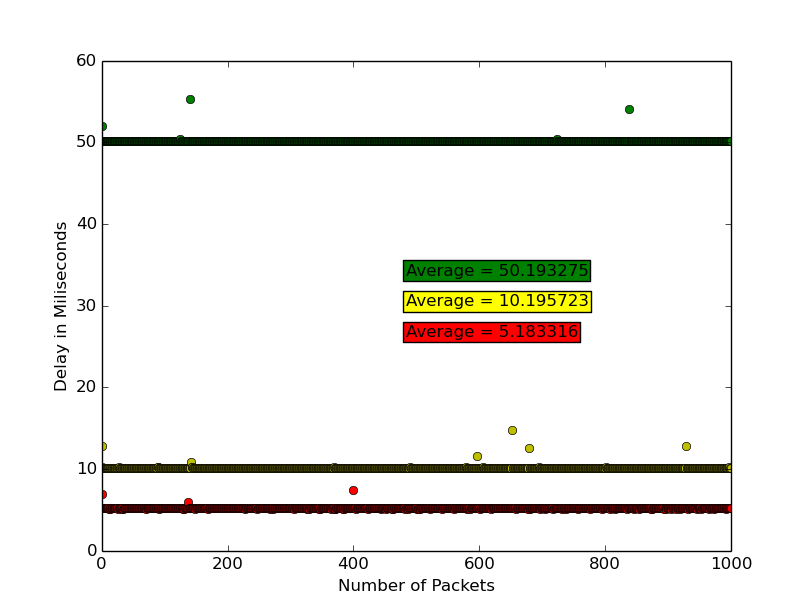
\includegraphics{delayplot-3-1-1000.png}}
		\caption{Delay for single flow.}
		\label{fig:delayplotsingle}
	\end{center}
\end{figure}

To test that script, I set up an emulation environment without dynamic DFG generation, configure the traffic control objects in the LCAs, and then execute that script from a node targeting its LCA. I ran the script for 5ms, 10ms, and 50ms delay. Figure \ref{fig:delayplotsingle} shows the time difference plotted for 5ms (red), 10ms (yellow), and 50ms (green) of delay for all 1,000 packets. I observed an average extra time of 200 microseconds taken for each packet and I assumed that this extra time includes sending the packet to the server, the latency between the client and server, processing at the server, receiving the packet at the client, and calculating and saving the time difference.
\begin{figure}[tb]
	\begin{center}
		\resizebox{\textwidth}{!}
		{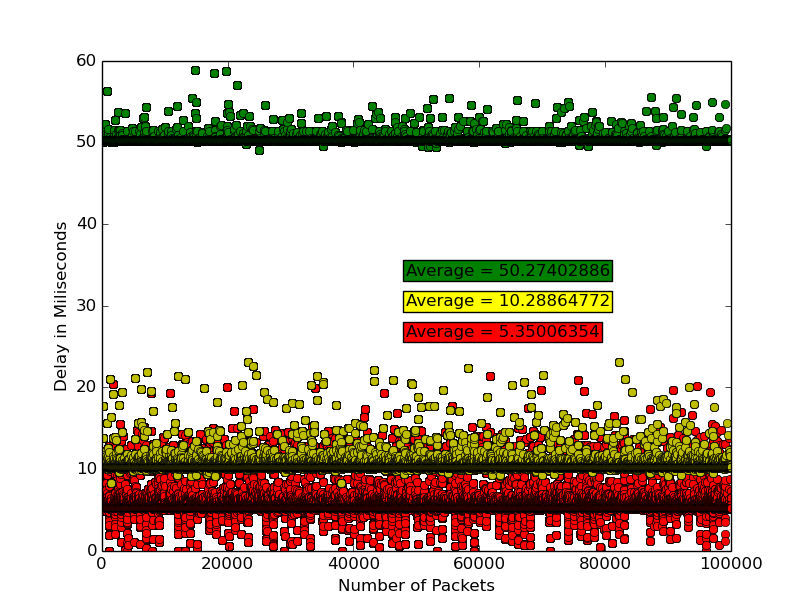
\includegraphics{delayplot-3-100-1000.png}}
		\caption{Delay for multiple flows.}
		\label{fig:delayplotmulti}
	\end{center}
\end{figure}

Similarly, I developed another small python script for testing packet loss and also to test the performance of the DFG processing capability when there is multiple parallel flow transmission happening. This script spawn 100 child processes executing the previous script. This means that in this case, there are 100 connections between a node and its LCA and each connection sends 1,000 packets one after another and save the time difference between sending and receiving of packets.

Same set up is used like the previous one to execute this multi-connection script. For most of the execution, the client could establish all 100 connections and receive returned packet for all the packets sent, which is why it could calculate the time difference for each packet. This also means there is no packet loss in the network. There are some occurrences where some clients could not establish the connection (3-4 out of 100); this might happen while the socat listener is busy serving another request. Figure \ref{fig:delayplotmulti} shows the time difference plotted for 5ms (red), 10ms (yellow), and 50ms (green) of delay for all $100\times1,000$ packets. In this case, I observed an average extra time of 300 microseconds taken for each packet.

I observed a similar pattern in both Mininet and MaxiNet platforms; here the given plot is generated in a MaxiNet platform where the source node and the LCA are running in the different MaxiNet worker.

\subsection{Traffic Generation Test}
I am using iperf to generate UDP traffic in the testbed and while starting iperf client instance, two parameters was passed, one for specifying data rate and one for the duration (see Section \ref{sec:tragen}). I saved the log for each iperf instance run and generated a report based on that log file for every evaluation scenario I executed.

\begin{figure}[tb]
	\begin{center}
		\resizebox{\textwidth}{!}
		{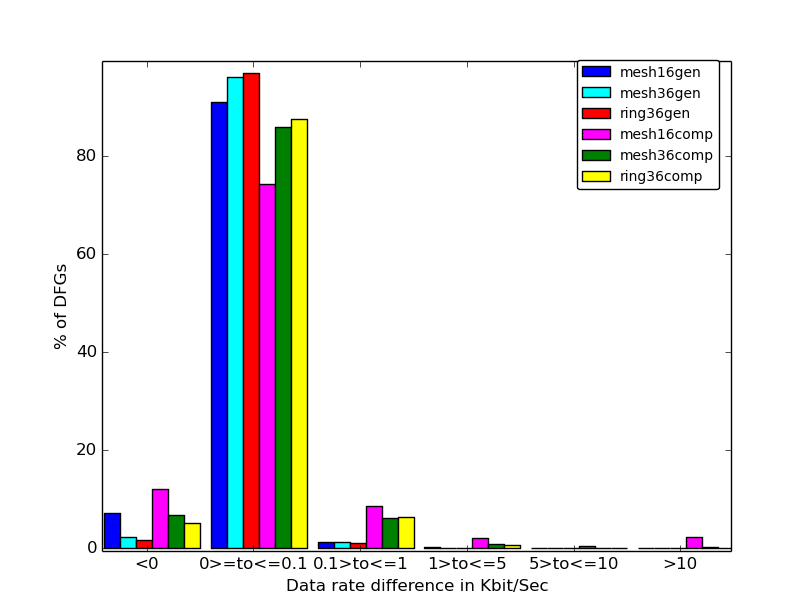
\includegraphics{bandwidthdiff.png}}
		\caption{Desired data rate vs generation data rate.}
		\label{fig:bandwidthdiff}
	\end{center}
\end{figure}

\begin{figure}[tb]
	\begin{center}
		\resizebox{\textwidth}{!}
		{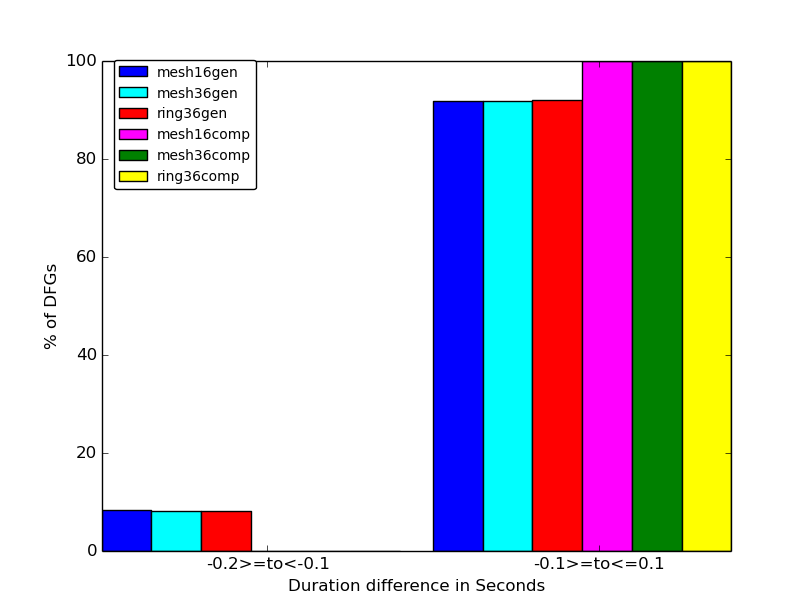
\includegraphics{timediff.png}}
		\caption{Expected duration vs generation duration.}
		\label{fig:timediff}
	\end{center}
\end{figure}

Figure \ref{fig:bandwidthdiff} shows the chart of expected data rate vs the actual data rate achieved while generating traffic. In Scenario 1 (blue) (see Table \ref{tab:evalscen}), the difference between desired data rate and generation data rate is 91\% of DFG between 0 to 0.1Kb/sec, 7\% less than 0Kb/sec (i.e., more data rate generated than expected), and 1\% greater than 0.1kb/sec. Iperf usually does not take the exact value for data rate or duration specified via command line but does some rounding of the specified value. For example, an iperf instance started with -b 9076381.59126 (data rate) and -t 45.26262756281 (duration), but iperf generated traffic of 9076386 bits/sec for 45.3 seconds. Another case, the iperf instance started with -b 9736626.21994 and -t 6.6471337635, but iperf generated traffic of 9736568bits/sec for 6.6 seconds. Thus, it is expected that iperf will sometimes round to a higher value and sometimes lower value. Similar data rate difference pattern to scenario 1 is observed in scenario 3 (cyan) and 4 (red). For scenario 2 (magenta), 5 (green), and 6 (yellow), the number of flow with a difference of 0.1 Kb/sec to 1Kb/sec is higher and the number of flows with the difference of less than 0Kb/sec also higher. These are CoMP scenarios and it demands higher data rate. This means iperf rounding may occur in higher range in both directions (negative or positive) if higher value passed with -b option while starting the iperf instance but none of the scenario show a huge difference between the desired rate and achieved rate. This proves that the data rate control of flow generation is working as expected in the testbed.

Figure \ref{fig:bandwidthdiff} shows the chart of expected duration of traffic generation vs actual duration for which actually the generation happened. In scenario 1 (blue) (see Table \ref{tab:evalscen}), for 92\% DFG the difference is in the range between -0.1 to 0.1 sec and 8\% DFG in the range of greater than -0.2 to less than -0.1 sec (a negative difference means traffic generation for more time than expected). A similar pattern is observed in scenario 3 (cyan) and 4 (red). For scenario 2 (magenta), 5 (green), and 6 (yellow), 100\% DFGs are in range of -0.1 to 0.1 sec difference. Even though for data rate, iperf round the passed value in both directions, i.e., either in lower or higher value, but usually iperf rounds the time parameter in higher value than it specified. This is the reason I observed for almost all the DFG; the difference between desired duration and generation duration is either 0 or negative. Though the rounding happens in ms range, there is not a single instance where the duration difference is very high. This proves that the duration control of flow generation is working as expected.

\subsection{Traffic Path Test}
FlexFCAPF decides the path for each DFG to follow, and based on the provided path, I added the forwarding entries in the underlying network elements. To verify whether the forwarding entries are correctly configured as per the path specified, I used \textit{Wireshark}. Figure \ref{fig:trafficpath} shows dump of UDP packet starting from host with IP 10.0.0.9 to destination host with IP 10.0.0.4. FlexFCAPF algorithm assigned the path to follow is: $s_8$ to $s_4$ to $s_3$; accordingly, the forwarding entries are added in the switches. Host 10.0.0.9 is connected to interface id 0 of $s_8$, $s_4$ is connected to the interface id 2 of $s_8$, $s_8$ is connected to interface id 11 of $s_4$, $s_3$ is connected to interface id 12 of $s_4$, $s_4$ is connected to interface id 13 of $s_3$ and host 10.0.0.4 is connected to interface id 7 of $s_3$.

\begin{figure}[tb]
	\begin{center}
		\resizebox{\textwidth}{!}
		{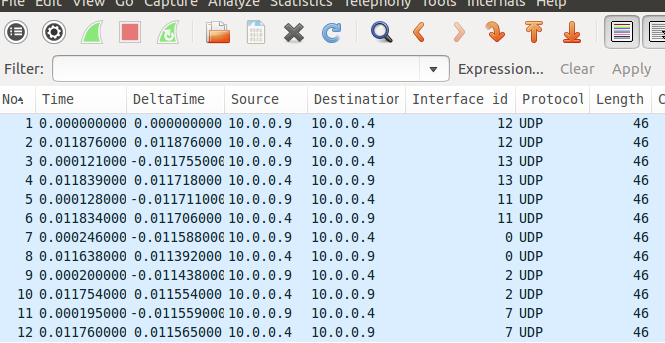
\includegraphics{h8toh3viah4.png}}
		\caption{Wireshark dump of a packet.}
		\label{fig:trafficpath}
	\end{center}
\end{figure}
In the Wireshark dump, we can see two packets passed through each of the interface, one with source IP 10.0.0.9 and destination IP 10.0.0.4, and another with source IP 10.0.0.4 and destination IP 10.0.0.9. This information proves two points: first the generated traffic follows exactly the path I configured and second, each packet goes to the destination (i.e., LCA) and LCA reply the same packet (same size of 46 Byte) back to the source. This is the kind of a DFG processing I wanted to implement in LCA.

\section{Reports Generation and Result Analysis}\label{sec:rgra}
I saved different dynamic statistics during execution of the scenarios specified in section \ref{sec:expscn} and based on those statistics, I generated some reports which I describe in this section.

As I already outlined in Section \ref{sec:expscn}, time difference ($t_d$) means emulation time ($t_e$) - system time passed from the start($t_s$). For example, I start an emulation at 3:00:00 PM for 2 hours (7,200 seconds); after some time, I got $t_e = 305$ and 3:05:00 PM is registered in the system clock time. This means the system clock moved 5 minutes (300 seconds) or equivalent to $t_s = 300$, so $t_d = t_e - t_s$ (i.e., $t_d=305-300=5$). Consider another situation, where I got $t_e=590$ and retrieved system clock time 3:10:00 PM. This means from the start the system time moved 10 minutes so $t_s=600$, and in this case $t_d=590-600=-10$. As I mentioned earlier, if the emulation time moved ahead of the system time (i.e., $t_d$ is positive), the emulation sleeps for the time difference and if emulation time is behind (i.e., $t_d$ is negative), then I assume emulation time will catch up with the system time.

Another terminology I used in this section is run-time ($t_r$). This is basically the length of real-time a process took to complete its task. I plotted two run-time for all the execution, one for algorithm run-time ($t_{ar}$) and another for reconfiguration run-time ($t_{rr}$). The $t_{rr}$ includes time spent on modifying routing path, configuring traffic control objects, and starting iperf instances needed after the execution of FelxFCAPF algorithm.

I collected all the time statistics before the emulation goes to sleep (if required) and all the plot I made in this section keeps emulation time ($t_e$) in the x-axis.

\subsection{Test Scenario 1}
This scenario was executed in Mininet platform with load level scale set to 0.40, mesh topology was used and the type of flow generated for the scenario is generic. Figure \ref{fig:ts1timediff} shows the plotting of $t_d$ against $t_e$. I observed both positive and negative $t_d$, which means occasionally $t_s$ is behind of $t_e$ or vice versa. A range of +1.34 to -1.23 seconds $t_d$ was observed. This is an expected behavior when there are many DFG added in the system which means more processing time is needed to configure traffic control objects and start iperf instances because of that $t_s$ moves ahead of $t_e$ and when few DFG is added in the system, $t_s$ is behind $t_e$ and the emulation would sleep for the $t_d$.

\begin{figure}[H]
	\begin{center}
		\subfloat[Emulation time vs time difference]{
			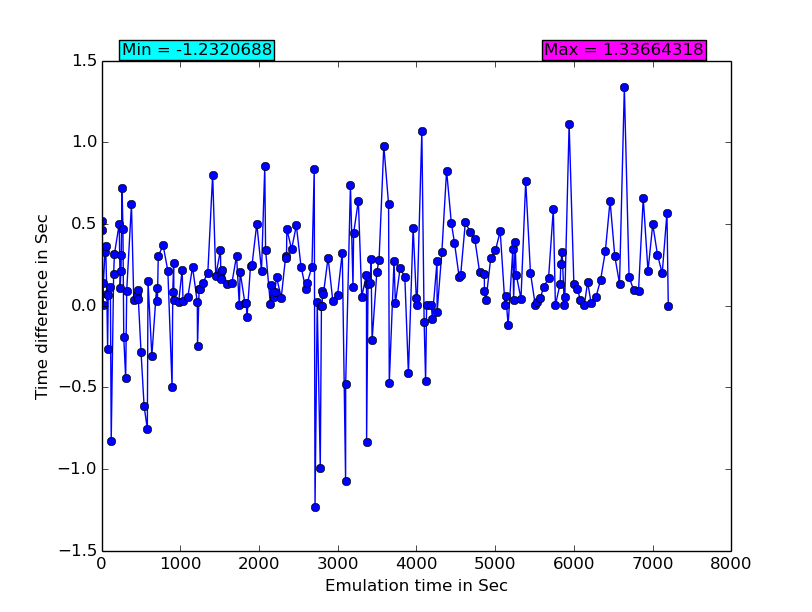
\includegraphics[width=0.48\textwidth]{16mesh40gentimediff.png}
			\label{fig:ts1timediff}
		}
		\subfloat[Emulation time vs runtime]{
			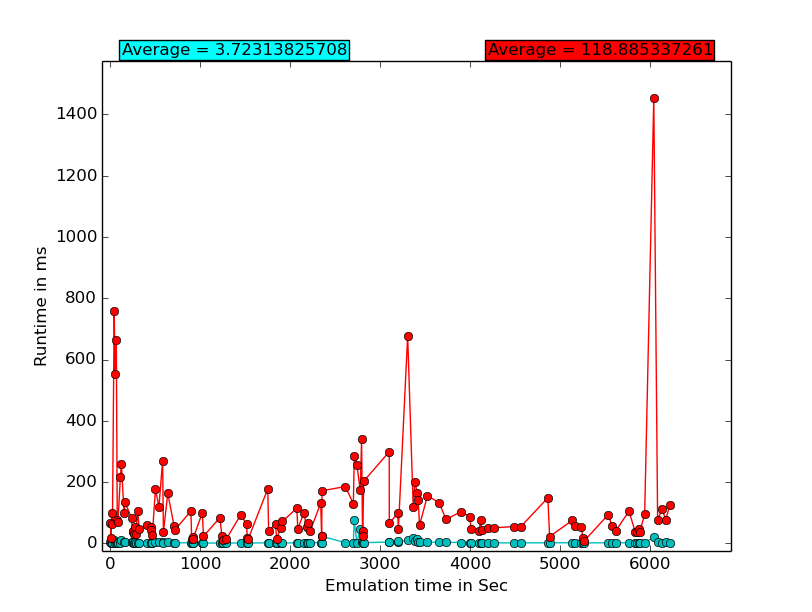
\includegraphics[width=0.48\textwidth]{16mesh40genruntime.png}
			\label{fig:ts1runtime}
		}
	\end{center}
\end{figure}

Figure \ref{fig:ts1runtime} has two statistics: the plotting of $t_{ar}$ against $t_e$ (cyan) and $t_{rr}$ against $t_e$ (red). Average $t_{ar}$ is around 3.72 ms whereas the average $t_{rr}$ is around 118.89 ms. Though the emulation for this scenario was executed for 7,200 seconds, the last algorithm execution was observed at 6,219 seconds, since there has been no more reassignment after this. There is few big spike of $t_{rr}$ seen, which means in that algorithm run, there are many DFG reassigned, which is why the system took more time to reset the routing entries, configure traffic control objects, and start iperf instances.

\subsection{Test Scenario 2}
This scenario was also executed in Mininet platform, the load level scale was set to 0.05, mesh topology was used and the type of flow generated for the scenario is CoMP. Figure \ref{fig:ts2timediff} shows the plotting of $t_d$ against $t_e$. Both positive and negative $t_d$ of +10.34 to -31.74 seconds is observed in this scenario. Here, $t_d$ has bigger range since it is a CoMP scenario; when there is heavy load the testbed has to start many iperf instances and configure many traffic control objects. This task takes time which is why more $t_s$ has passed while $t_e$ does not move much. In another case, while load level scale is low (0.05), then the emulation has to add very few DFG in the system because of that $t_e$ move ahead of the system time.

\begin{figure}[H]
	\begin{center}
		\subfloat[Emulation time vs time difference]{
			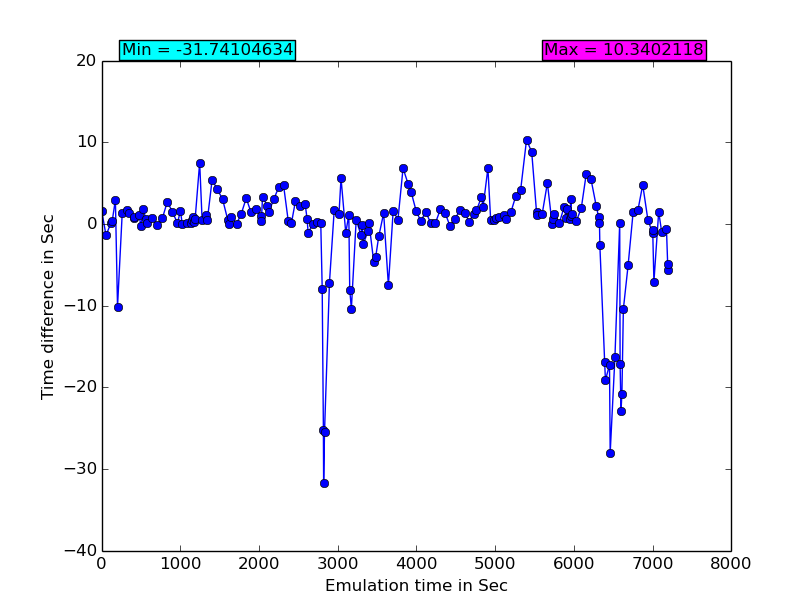
\includegraphics[width=0.48\textwidth]{16mesh05comptimediff.png}
			\label{fig:ts2timediff}
		}
		\subfloat[Emulation time vs runtime]{
			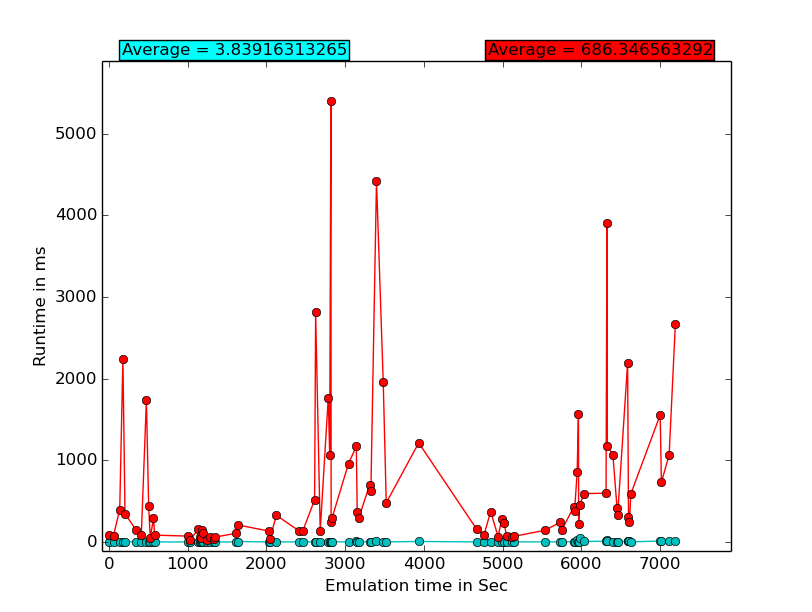
\includegraphics[width=0.48\textwidth]{16mesh05compruntime.png}
			\label{fig:ts2runtime}
		}
	\end{center}
\end{figure}

Similar to scenario 1, Figure \ref{fig:ts2runtime} has two statistics: the plotting of $t_{ar}$ against $t_e$ (cyan) and $t_{rr}$ against $t_e$ (red). Average $t_{ar}$ is around 3.83 ms and the average $t_{rr}$ is around 686.34 ms. The average $t_{rr}$ is higher because for CoMP flow type, usually numerous traffic control objects need to be added, and for a single DFG, multiple traffic flow generation has to be started. Similar to scenario 1, there are few big spikes of $t_{rr}$ seen, which means in that algorithm run, there were many DFGs reassigned. Compared to scenario 1, here I observed bigger gaps between the dots, which means less number of algorithm execution has happened.

\subsection{Test Scenario 3}
This scenario was executed in MaxiNet platform, the load level scale was set to 0.20, mesh topology was used, and the type of flow generated for the scenario is generic. Figure \ref{fig:ts3timediff} shows the plotting of $t_d$ against $t_e$. Both positive and negative $t_d$ of +0.89 to -0.73 seconds was observed in this scenario. Since load scale is medium and flow type is generic, a low range $t_d$ has been observed in this case.

\begin{figure}[H]
	\begin{center}
		\subfloat[Emulation time vs time difference]{
			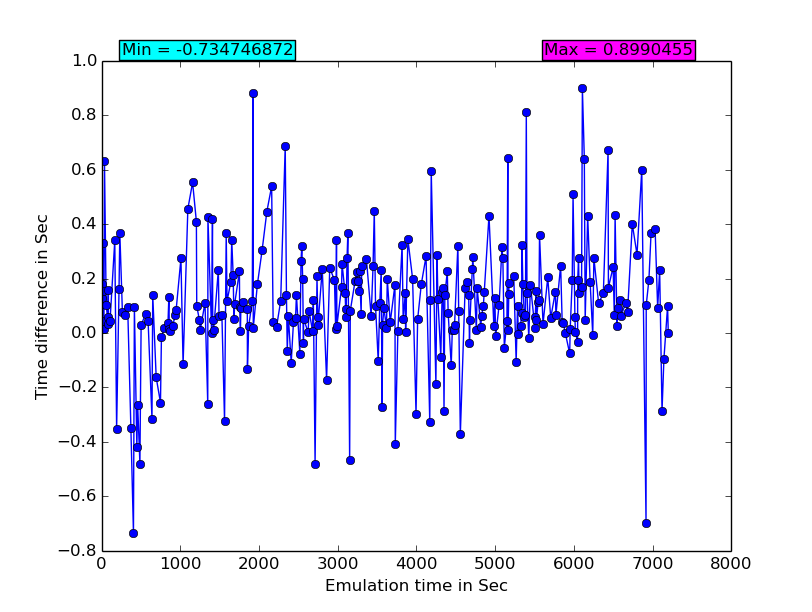
\includegraphics[width=0.48\textwidth]{36mesh20gentimediff.png}
			\label{fig:ts3timediff}
		}
		\subfloat[Emulation time vs runtime]{
			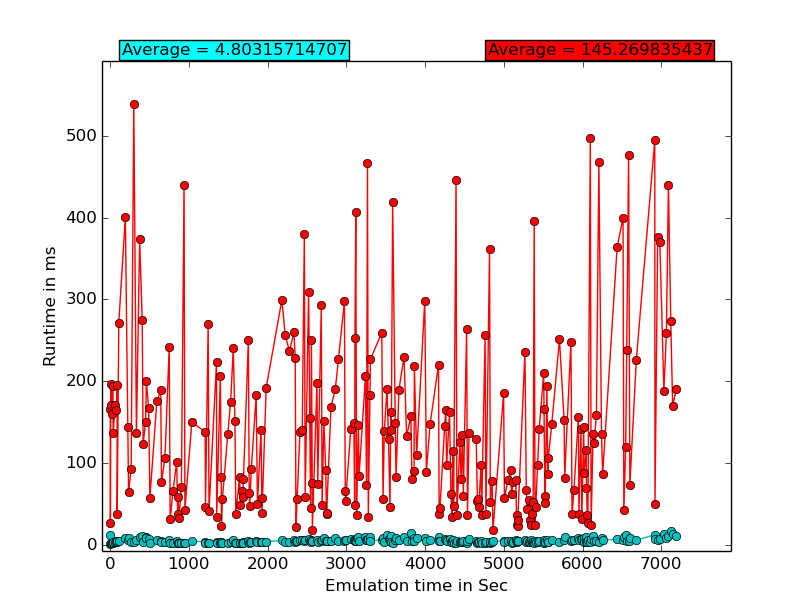
\includegraphics[width=0.48\textwidth]{36mesh20genruntime.png}
			\label{fig:ts3runtime}
		}
	\end{center}
\end{figure}

Similar to other scenarios Figure \ref{fig:ts3runtime} has two statistics: the plotting of $t_{ar}$ against $t_e$ is in cyan and $t_{rr}$ against $t_e$ is in red. Average $t_{ar}$ is around 4.08 ms and the average $t_{rr}$ is around 145.27 ms. The average $t_{rr}$ is low because for generic flow types, very few traffic control objects are needed to create since most DFG have similar processing delay. Like the other generic scenario, I also observed here fewer gaps between dots, which means the algorithm execution happened very frequently.

\subsection{Test Scenario 4}
This scenario was also executed in MaxiNet platform, the load level scale was set to 0.20, a ring topology was used and the type of flow generated for the scenario is generic. Figure \ref{fig:ts4timediff} shows the plotting of $t_d$ against $t_e$. Both positive and negative $t_d$ of +1.43 to -0.91 seconds was observed in this scenario. Similar to scenario 3, the load scale is medium and flow type is generic so a low range $t_d$ was observed in this case.

\begin{figure}[H]
	\begin{center}
		\subfloat[Emulation time vs time difference]{
			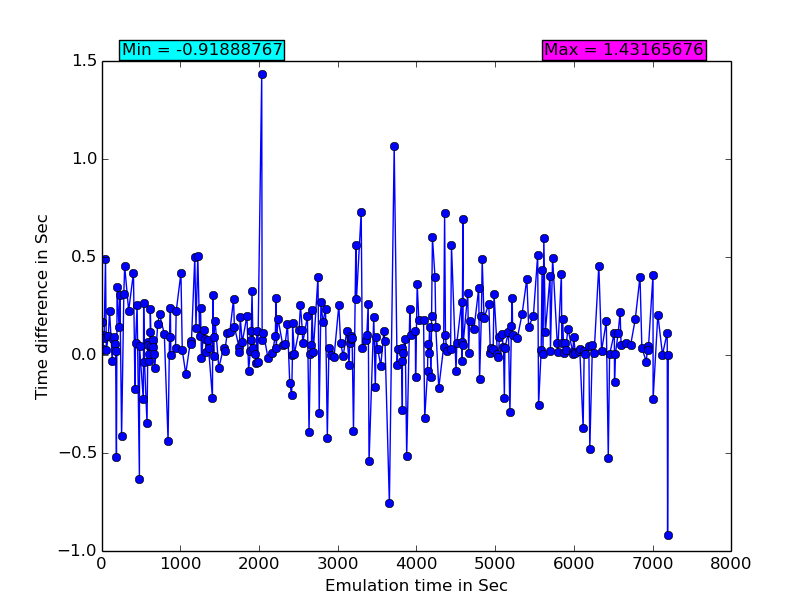
\includegraphics[width=0.48\textwidth]{36ring20gentimediff.png}
			\label{fig:ts4timediff}
		}
		\subfloat[Emulation time vs runtime]{
			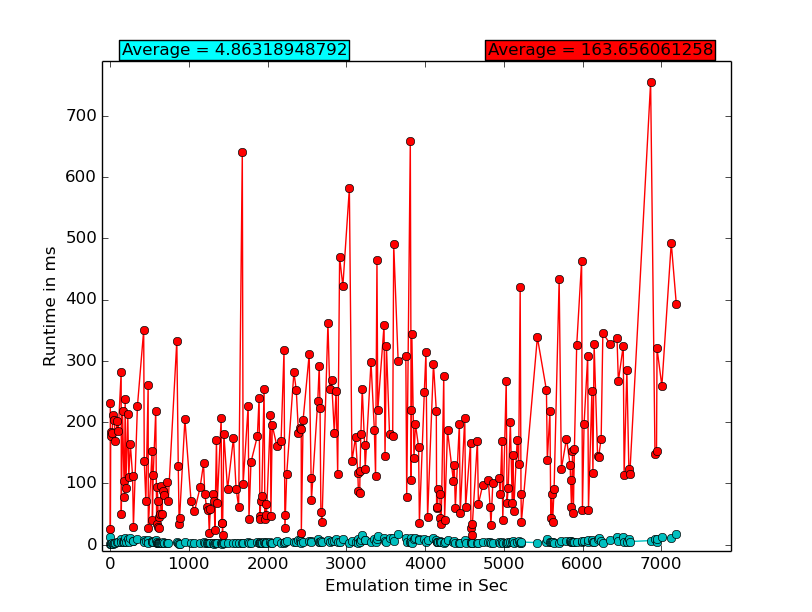
\includegraphics[width=0.48\textwidth]{36ring20genruntime.png}
			\label{fig:ts4runtime}
		}
	\end{center}
\end{figure}

Similar to other scenarios, Figure \ref{fig:ts4runtime} has two statistics: the plotting of $t_{ar}$ against $t_e$ is in cyan and $t_{rr}$ against $t_e$ is in red. Average $t_{ar}$ is around 4.86 ms and the average $t_{rr}$ is around 163.65 ms. Similar to scenario 3, the average $t_{rr}$ is low because of generic flow type. Like other generic scenarios, here the algorithm execution also happened very frequently.

\subsection{Test Scenario 5}
This scenario was also executed in MaxiNet platform, the load level scale was set to 0.02, mesh topology was used and the type of flow generated for the scenario is CoMP. Figure \ref{fig:ts5timediff} shows the plotting of $t_d$ against $t_e$. Both positive and negative $t_d$ of +11.51 to -3.87 seconds was observed in this scenario. Here, $t_d$ has bigger range since it is a CoMP scenario; when the load is higher, the testbed has to start many iperf instances and configure many traffic control objects which is why more system time passed while the $t_e$ does not move that much. In another case, while load level scale is low (0.02), then the emulation has to add very few flow in the system because of that $t_e$ move ahead of $t_s$.

\begin{figure}[H]
	\begin{center}
		\subfloat[Emulation time vs time difference]{
			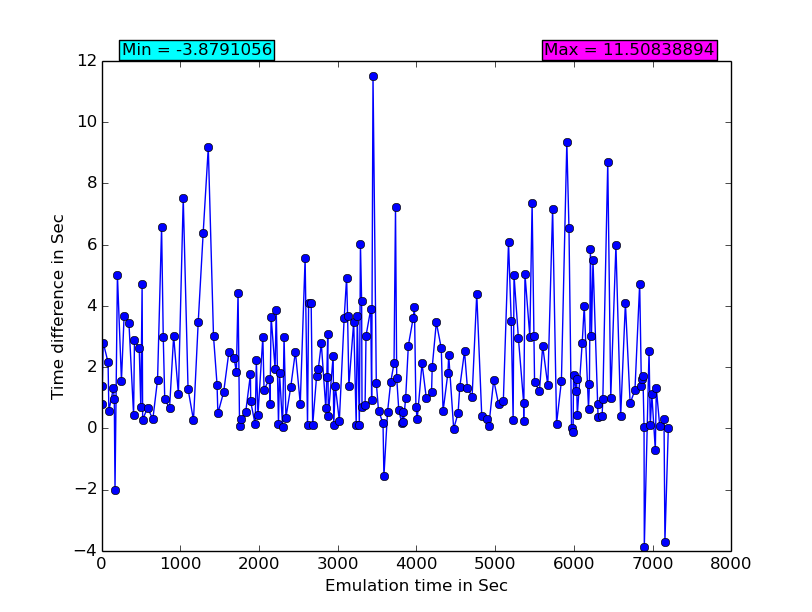
\includegraphics[width=0.48\textwidth]{36mesh02comptimediff.png}
			\label{fig:ts5timediff}
		}
		\subfloat[Emulation time vs runtime]{
			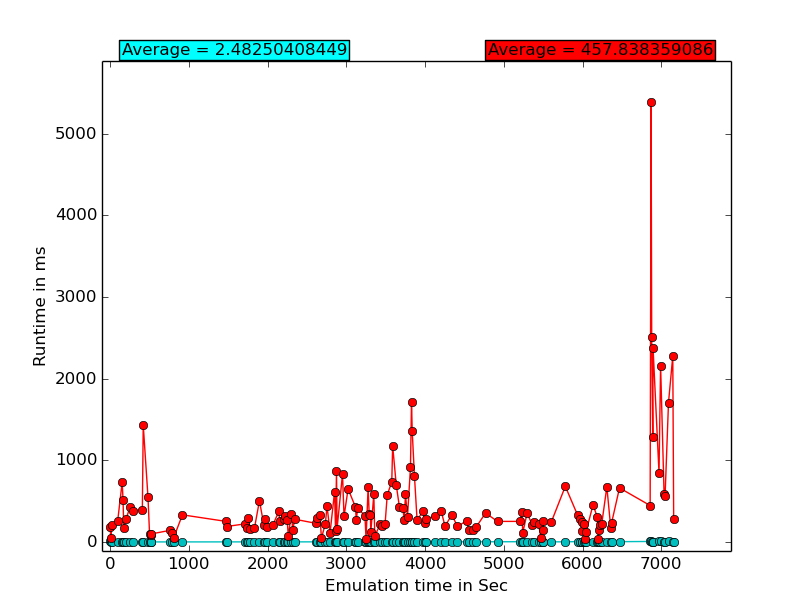
\includegraphics[width=0.48\textwidth]{36mesh02compruntime.png}
			\label{fig:ts5runtime}
		}
	\end{center}
\end{figure}

Similar to other scenarios, Figure \ref{fig:ts5runtime} has two statistics: the plotting of $t_{ar}$ against $t_e$ is in cyan and $t_{rr}$ against $t_e$ is in red. Average $t_{ar}$ is around 2.48 ms and the average $t_{rr}$ is around 457.83 ms. The average $t_{rr}$ is higher because for CoMP flow types, numerous traffic control objects are usually need to be added and for a single DFG, multiple traffic flow generation has to be started. Like other CoMP scenarios, here I observed bigger gaps between the dots, which means less number of algorithm execution happened. I observed a big spike for $t_{rr}$ at the end, which happened because at that algorithm execution, 2 LCA were removed at a time due to low load situation. This means there were many changes in the node to LCA assignment so there are many routing entry needed to be added and deleted in the underlying network. Additionally, there are many DFG which were reassigned, therefore many iperf instances that need to be started.For this reason, the emulation took a lot of time to process those tasks and $t_{rr}$ rose to 5,382 ms.

\subsection{Test Scenario 6}
This scenario was also executed in MaxiNet platform, the load level scale was set to 0.02, a ring topology was used and the type of flow generated for the scenario is CoMP. Figure \ref{fig:ts6timediff} shows the plotting of $t_d$ against $t_e$. Both positive and negative $t_d$ of +13.33 to -0.34 seconds was observed in this scenario. Similar to scenario 5, the load scale is low and flow type is CoMP so a higher range of $t_d$ has been observed in this case.

\begin{figure}[H]
	\begin{center}
		\subfloat[Emulation time vs time difference]{
			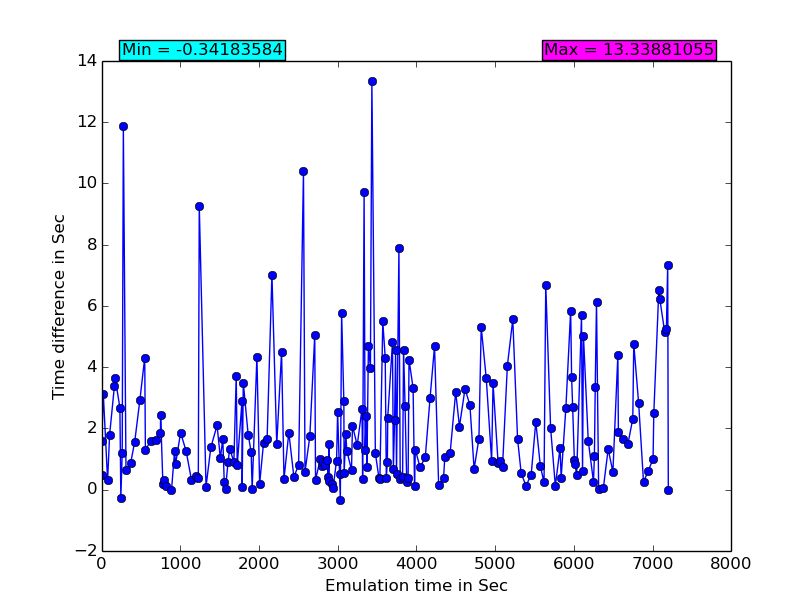
\includegraphics[width=0.48\textwidth]{36ring02comptimediff.png}
			\label{fig:ts6timediff}
		}
		\subfloat[Emulation time vs runtime]{
			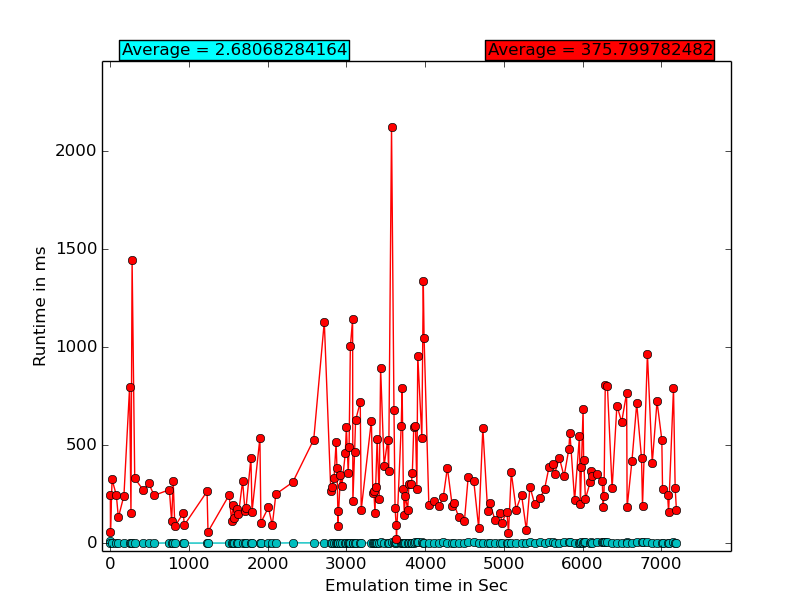
\includegraphics[width=0.48\textwidth]{36ring02compruntime.png}
			\label{fig:ts6runtime}
		}
	\end{center}
\end{figure}

Similar to other scenarios, Figure \ref{fig:ts6runtime} has two statistics: the plotting of $t_{ar}$ against $t_e$ is in cyan and $t_{rr}$ against $t_e$ is in red. Average $t_{ar}$ is around 2.68 ms and the average $t_{rr}$ is around 375.79 ms. Similar to scenario 5, average $t_{rr}$ is high because of the CoMP flow type, and bigger gaps between algorithm run has been observed here as well. 

Usually, in the generic scenario, algorithm runs happen very frequently which means many reassignments happen and which is why there are many fluctuating spikes seen in $t_{rr}$ plotting. Whereas in the case of CoMP scenario, the number of algorithm run was lesser which is why bigger gaps between dots have been observed in $t_{rr}$ plotting. Even though there are very few long spikes in CoMP scenario, the average $t_{rr}$ is very high which means for CoMP scenario there are many traffic control objects to configure and many iperf instances to start after the algorithm run. Another important observation in CoMP scenario is a high range of $t_d$ due to the lesser number of DFG to be added in the system, though the number of traffic control objects to configure and the number of iperf instances to be run is higher which caused higher $t_d$ range. A common pattern is observed across all scenarios, all $t_{rr}$ plotting followed the load level curve specified in Figure \ref{fig:24loadlevel}. Initially, the load is high in the system so $t_{rr}$ is high; it goes down to lowest around 900 seconds then it starts increasing and reach high at around 3,500 seconds and again start decreasing and goes down to lowest around 4,500 seconds and reach high again at around 7,000 seconds.

\section{Comparison with Simulation}\label{sec:cws}
I did not modify the actual FlexFCAPF algorithm for emulation. The algorithm was executed in simulation and the evaluation results of the simulation are presented in \cite{7343600}. I mainly focused on evaluating emulation aspects which were not possible in the simulation. Virtual network elements and hosts are created in the emulation testbed and real application is running on them (ipref, Wireshark, socat, etc.). Actual OpenFlow protocol is used to communicate between the SDN controller and the network elements. The real forwarding entries are populated in the network elements and tested traffic is following the exact path as specified. A real data processing capability is implemented, real traffic is generated and transmitted between hosts, and verified that the traffic bandwidth and duration can be controlled as desired. Finally, the emulation evaluation scenarios are executed in real time so the algorithm performance is proven in a more realistic environment.
\begin{figure}[H]
	\begin{center}
		\subfloat[Simulation time vs number of LCA used]{
			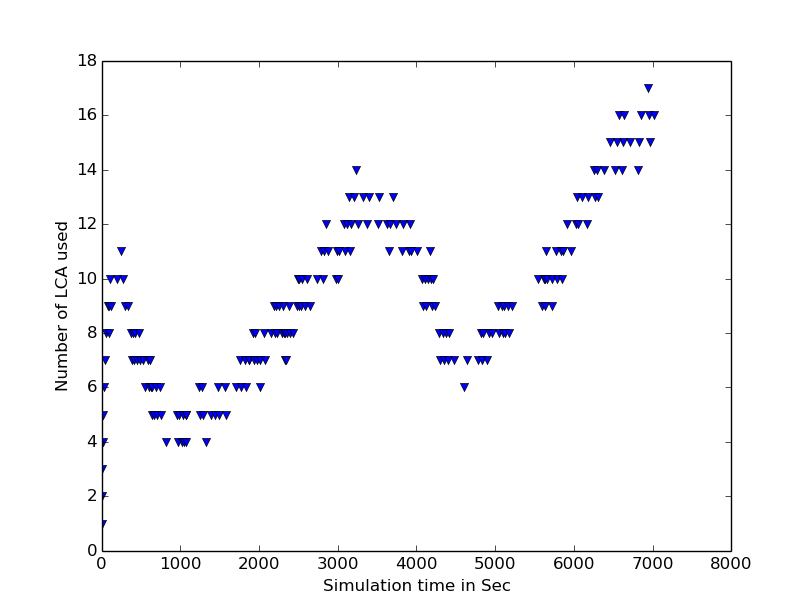
\includegraphics[width=0.48\textwidth]{sim-lcaused.png}
			\label{fig:simlca}
		}
		\subfloat[Emulation time vs number of LCA used]{
			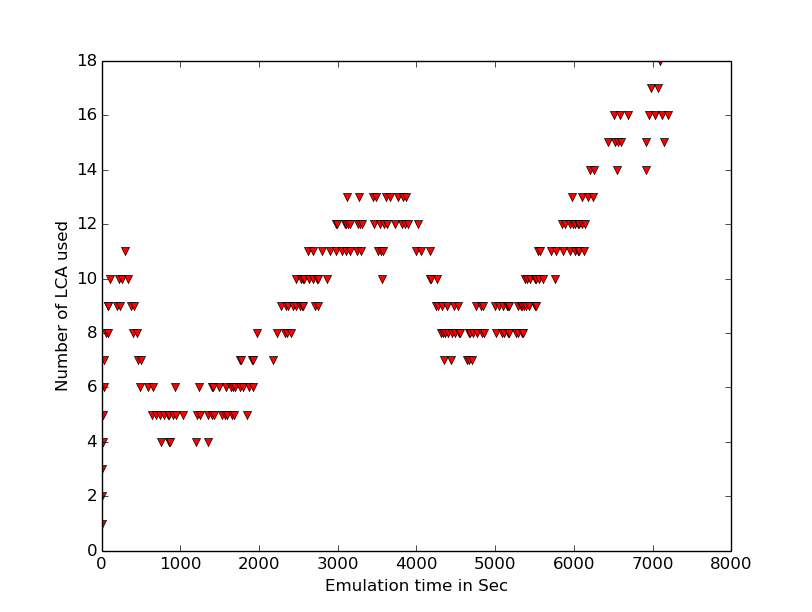
\includegraphics[width=0.48\textwidth]{emu-lcaused.png}
			\label{fig:emulca}
		}
	\end{center}
\end{figure}

I executed a scenario to show that the outcome of the algorithm is independent of the simulation or emulation. Figure \ref{fig:simlca} and \ref{fig:emulca} show the number of LCA used in simulation and emulation execution, respectively. Both simulation and emulation are executed for 7,200 seconds using same topology description (mesh) with 36 nodes and generic type DFG are added during the execution. I observed similar number of LCA used in both cases and LCAs are adjusted in similar pattern during the complete execution.
         % Chapter 4
% chap5.tex (Conclusion)
\newpage
\thispagestyle{empty}
\mbox{}


\chapter{Conclusion \& Future Work} \label{CONC-CHAP}

\section{Conclusion}
I built an SDN-based emulation testbed which is flexible, realistic, scalable and agile. Any kind of network topology can be created and execute experiment on it. A flexible way for manipulating the load level is defined. It is possible to use either Mininet or MaxiNet emulation framework to create an emulation network, run any SDN controller and control the link bandwidth and CPU power if necessary. The testbed is designed to evaluate any FCAPP solution approach.

The testbed provides almost similar functionality as a real hardware network. It runs a real SDN controller which has the capability of discovering the underlying network and has a REST interface to accept a request from other applications and implement it in the underlying network. The testbed supports real traffic generation and traffic characteristics (data rate, duration) can be controlled. It is also possible to pass user defined identifier in the packet of the generated traffic. The testbed has a high fidelity data processing capability which is implemented in a very lightweight manner, it takes very less (almost negligible) processing power of the hardware. The testbed also has the ability to receive and regenerate real traffic. Most importantly, experiments can be executed in real time.

The testbed is designed to be highly scalable; it is possible to create a network with just 9 nodes and the number of nodes can be increased to 64 nodes with low load level. But this constraint is due to limited hardware capacity; it is possible to prepare a network of thousands of nodes with a right amount of hardware.

The testbed source code is not dependent on the hardware. It is possible to move the source code to any system with Debian 8.0 and Ubuntu 14.04 and execute emulation.

Different tests have been executed to verify if all the aforementioned functionalities are working. To verify controller functionality a test has been executed and demonstrated that the traffic in the underlying network follows the right path as specified. Traffic generation logs are saved for the whole experiment executed and later verified that more than 90\% of real traffic generation happened as desired. Multiple traffic control objects are configured in the same interface and packet are passed through it; it has been observed that right delay has been applied to each packet passing through that interface based on the packet identifier. To verify the data processing capability under high load situation, 100 parallel connections were established between two nodes and 1,000 packets were transferred between them. It was observed that the right average delay was applied to all the packets as specified and 0\% packet loss was observed.

A varying load level is maintained during the whole execution and it is observed that FlexFCAPF algorithm successfully adjust the network based on the load level in the system. This proves that FlexFCAPF is a feasible solution in more realistic network setup (i.e., emulation). It was observed that even at the peak load situation FlexFCAPF does not take more than 20 ms to reconfigure the whole network. No dereference was observed in terms of performance of the algorithm execution in simulation and emulation. A similar amount of LCA was used for test execution with similar kind of load level in both simulation and emulation. These evaluations prove that functionality wise, FlexFCAPF is working correctly.

\section{Future Work}
Even though I successfully achieved all the goals of my thesis, I still observed some aspects during the course of the thesis which could be tackled in future research. The Ryu SDN controller used cannot survive for long hours if the load in the testbed is high. There is a problem in the SDN controller when multiple connection requests come from the network elements with same DPID. This situation was observed when there is huge load in the OVS, it restarts (see Section \ref{sec:expscn}) and causes multi-connection problem. This kind of problem can be analysed easily if a monitoring tool (e.g., Ntop \cite{ntop}, Zenoss \cite{zenoss}) is running on the testbed. A monitoring tool not only identify problems it can also be used to see real time statistics of traffic flows, load on a network elements and many more. Running any network monitoring tool would need lot of hardware resources. 

Currently, I am using iperf for traffic generation and socat as traffic receiver. With this setup, it is not possible to track each and every packet from source node to the destination, which is why I could not measure the packet loss in the network (if any) for the whole execution of the experiments. A possible, yet labor-intensive solution would be to develop a custom traffic generator and traffic receiver like iperf so that one can track each packet travelling in the network and calculate packet loss for the whole experiment execution. 

A real data processing application can be implemented in the testbed (e.g., a simple traffic summary aggregator or a complex data encryption application), provided the right amount of hardware resource is available in the testbed. Right now RCA has no realistic significance in the testbed. Since the SDN controller has a complete view of the network, a logical connection can be created between the RCA and the SDN controller to have a realistic implementation.

\newpage
\thispagestyle{empty}
\mbox{}
         % Chapter 5
%\include{chapter6}         % Chapter 6
%\include{chapter7}         % Chapter 7, chap7.tex contains an
                        % example of figs and tables and inclusion of pdf.

%%%%%%%%%%%%%%%%%%%%
% Concluding Pages %
%%%%%%%%%%%%%%%%%%%%%%%%%%%%%%%%%%%%%%%%%%%%%%%%%%%%%%%%%%%%%%%%%%%%%%%%%%%%%%%%

% Bibliography or References, REQUIRED

% If using bibtex, create or modify the refs.bib file
% and use (uncomment) the following three lines.
\bibliographystyle{plain}     %You may prefer \bibliographystyle{alpha}
\addcontentsline{toc}{chapter}{\bibname}
\bibliography{refs}         

% If using the ``thereference'' environment instead, modify the ref.tex file
% and use the following line
%\include{ref}

% If including appendices, uncomment the following lines,
% adding more includes if needed.
\StartAppendix
% appendix.tex (Appendix)
\newpage
\thispagestyle{empty}
\mbox{}


\chapter{Appendix A}\label{APPD-CHAP}
This chapter covers the infrastructure and operation aspects of the testbed. It provides the hardware details along with basic structure and elements of the testbed. It also presents a stepwise procedure to install and configure the testbed as well as configure FlexFCAPF emulation.

\section{Infrastructure}\label{sec:infra}
Figure \ref{fig:testinfra} shows the overview of the current testbed infrastructure. The testbed consists of four physical machines (PC1, PC2, PC3, and PC4). All these four machines are connected to Paderborn University's network with an ethernet switch (20Gbits) using their internal Network Interface Cards (NICs). A terminal is connected to the first machine. A user can access the testbed using the terminal or using ssh through the university network. PC1 is used as MaxiNet frontend and the other three machines are used as MaxiNet worker. FlexFCAPF and the Ryu Controller Framework also run on PC1. Altogether, these machines build the MaxiNet Cluster. The system configuration of the testbed is described in Table \ref{tab:sysconf}.

\begin{table}[h!]
	\centering
	\caption{System configuration of testbed machine}
	\label{tab:sysconf}
	{\footnotesize
	\begin{tabular}{|c|c|c|c|c|c|c|}
		\hline
		\textbf{Details} & \textbf{CPU} & \textbf{Core} & \textbf{RAM} & \textbf{OS} & \textbf{Host Name} & \textbf{IP Address}\\
		\hline
		\textbf{PC1} & 3.00GHz & 2 & 4GB & Ubuntu 14.04 LTS & fg-cn-crowd-1.cs.upb.de & 131.234.250.30\\
		\hline
		\textbf{PC2} & 3.00GHz & 2 & 8GB & Ubuntu 14.04 LTS & fg-cn-crowd-2.cs.upb.de & 131.234.250.31\\
		\hline
		\textbf{PC3} & 3.00GHz & 2 & 8GB & Ubuntu 14.04 LTS & fg-cn-crowd-3.cs.upb.de & 131.234.250.32\\
		\hline
		\textbf{PC4} & 3.00GHz & 2 & 8GB & Ubuntu 14.04 LTS & fg-cn-crowd-4.cs.upb.de & 131.234.250.33\\
		\hline
		\multicolumn{7}{|c|}{All are Intel(R) Core(TM)2 Duo CPU E8400 processor}\\
		\hline
	\end{tabular}
	}
\end{table}

\section{Software Installation and Configuration}
All machines run on Ubuntu 14.04 LTS OS. The testbed has two user accounts configured, \textit{crowd} and \textit{maxinet}. The \textit{crowd} user can be used for running any application, including SDN Controller. On the other hand, the \textit{maxinet} user can execute commands as root with sudo without a password and is needed to run the MaxiNet emulation.

The following softwares are installed in the MaxiNet Frontend (PC1):

\begin{enumerate}
	\item Mininet v2.2.1
	\item Maxinet v1.0
	\item Metis v5.1
	\item Pyro v4.37
	\item Ryu v4.13
\end{enumerate}

Meanwhile, the following softwares listed below are installed in the MaxiNet Worker (PC2, PC3, and PC4):
\begin{enumerate}
	\item Mininet v2.2.1
	\item Maxinet v1.0
	\item Metis v5.1
	\item Pyro v4.37
	\item iperf v2.0.5 (Customized)
\end{enumerate}

I assumed that the version control utility \textit{git}, programming language \textit{Python v2.7.6}, and package manager \textit{pip} are already installed in all the machines. Below, I describe the installation instruction of the software mentioned above:

\paragraph{Metis:} 
The archived source code of \textit{Metis v5.1} was downloaded and installed (see Listing \ref{lst:metisi}). There is no specific configuration necessary for \textit{Metis}.

\begin{lstlisting}[caption={Metis nstallation},label={lst:metisi},language=bash,tabsize=2,basicstyle=\footnotesize,breaklines=true,showspaces=false,showstringspaces=false,showtabs=false,frame=single]
wget http://glaros.dtc.umn.edu/gkhome/fetch/sw/metis/metis-5.1.0.tar.gz
tar -xzf metis-5.1.0.tar.gz
cd metis-5.1.0
make config
make
sudo make install
\end{lstlisting}

\paragraph{Pyro:} 
The archived source code of \textit{Pyro v4.37} was downloaded and installed (see Listing \ref{lst:pyroi}). There is no specific configuration necessary for \textit{Pyro}.
\begin{lstlisting}[caption={Pyro installation},label={lst:pyroi},language=bash,tabsize=2,basicstyle=\footnotesize,breaklines=true,showspaces=false,showstringspaces=false,showtabs=false,frame=single]
git clone git://github.com/mininet/mininet
cd mininet
git checkout -b 2.2.1 2.2.1
cd util/
./install.sh
\end{lstlisting}

\paragraph{Mininet:} 
The latest source code from the \textit{Mininet} repository was downloaded and installed (see Listing \ref{lst:minineti}). There is no specific configuration necessary for \textit{Mininet}.
\begin{lstlisting}[caption={Mininet installation},label={lst:minineti},language=bash,tabsize=2,basicstyle=\footnotesize,breaklines=true,showspaces=false,showstringspaces=false,showtabs=false,frame=single]
git clone git://github.com/mininet/mininet
cd mininet
git checkout -b 2.2.1 2.2.1
cd util/
./install.sh
\end{lstlisting}

\paragraph{MaxiNet:} 
The latest source code from the \textit{MaxiNet} repository was downloaded and installed (see Listing \ref{lst:maxineti}).
\begin{lstlisting}[caption={MaxiNet installation},label={lst:maxineti},language=bash,tabsize=2,basicstyle=\footnotesize,breaklines=true,showspaces=false,showstringspaces=false,showtabs=false,frame=single]
git clone git://github.com/MaxiNet/MaxiNet.git
cd MaxiNet
git checkout v1.0
sudo make install
\end{lstlisting}

Since I am running Ubuntu, I have to set up a user (\textit{maxinet}) to use \textit{sudo} without password (see Listing \ref{lst:nopass}). This is done by adding the following line to in the \textit{/etc/sudoers} file.
\begin{lstlisting}[caption={Set no password},label={lst:nopass},language=bash,tabsize=2,basicstyle=\footnotesize,breaklines=true,showspaces=false,showstringspaces=false,showtabs=false,frame=single]
maxinet ALL=(ALL) NOPASSWD: ALL
\end{lstlisting}

The next thing I did was, copied the \textit{MaxiNet.cfg} to \textit{/etc/} and modified it (see Listing \ref{lst:cmaxinetc} and \ref{lst:emaxinetc}).
\begin{lstlisting}[caption={Copy MaxiNet configuration},label={lst:cmaxinetc},language=bash,tabsize=2,basicstyle=\footnotesize,breaklines=true,showspaces=false,showstringspaces=false,showtabs=false,frame=single]
sudo cp ~/MaxiNet/share/MaxiNet-cfg-sample /etc/MaxiNet.cfg
\end{lstlisting}

\begin{lstlisting}[caption={Edit MaxiNet configuration},label={lst:emaxinetc},language=bash,tabsize=2,basicstyle=\footnotesize,breaklines=true,showspaces=false,showstringspaces=false,showtabs=false,frame=single]
[all]
password = HalloWelt
controller = 131.234.250.30:6633
logLevel = INFO        ; Either CRITICAL, ERROR, WARNING, INFO  or DEBUG
port_ns = 9090         ; Nameserver port
port_sshd = 5345       ; Port where MaxiNet will start an ssh server on each worker
runWith1500MTU = True ; Set this to True if your physical network can not handle MTUs >1500.
useMultipleIPs = 0     ; for RSS load balancing. Set to n > 0 to use multiple IP addresses per worker. More information on this feature can be found at MaxiNets github Wiki.
deactivateTSO = True   ; Deactivate TCP-Segmentation-Offloading at the emulated hosts.
sshuser = maxinet         ; On Debian set this to root. On ubuntu set this to user which can do passwordless sudo
usesudo = True        ; If sshuser is set to something different than root set this to True.

[FrontendServer]
ip = 131.234.250.30

[fgcn-crowd-2]
ip = 131.234.250.31
share = 1

[fgcn-crowd-3]
ip = 131.234.250.32
share = 1

[fgcn-crowd-4]
ip = 131.234.250.33
share = 1
\end{lstlisting}

\paragraph{Ryu:} 
The latest source code from the \textit{Ryu} repository was downloaded and installed (see Listing \ref{lst:ryui}). There is no specific configuration necessary for \textit{Ryu}, but it is good to check if the \textit{/usr/local/etc/ryu/ryu.conf} has been configured for expected host and port. For example, FCAPF Network Controller is running on PC1 and it uses WSGI port 8080 and OpenFlow listen port 6633 and host as localhost, these are default Ryu settings. It is important to note that the OpenFlow listen host and port should match the \textit{MaxiNet} configuration, and WSGI host and port should match the FlexFCAPF configuration. FlexFCAPF uses this host and port information to call REST APIs provided by the FlexFCAPF Network Controller.
\begin{lstlisting}[caption={Ryu installation},label={lst:ryui},language=bash,tabsize=2,basicstyle=\footnotesize,breaklines=true,showspaces=false,showstringspaces=false,showtabs=false,frame=single]
git clone git://github.com/osrg/ryu.git
cd ryu
sudo pip install .
\end{lstlisting}

\paragraph{Iperf:} 
Standard \textit{iperf} is not suitable for the testbed I built because I need to add a \textit{bucket\_id} in the \textit{iperf} packet. The modified \textit{iperf} code is available in the \textit{FlexFCAPF} repository. The steps for building the \textit{iperf} from source code is as follows (see Listing \ref{lst:iperfi}):

\begin{lstlisting}[caption={Iperf installation},label={lst:iperfi},language=bash,tabsize=2,basicstyle=\footnotesize,breaklines=true,showspaces=false,showstringspaces=false,showtabs=false,frame=single]
git clone git@github.com:tarunsarkar/flexfcapf.git
cd flexfcapf/iperf2
./configure
make
cd ../
cp iperf2/src/iperf .
\end{lstlisting}

All the following scripts or executables are expected to be present inside \textit{flexfcapf} directory of the home directory of the \textit{maxinet} user. If not present, then the hard coded path in FlexFCAPF code referring them should be modified. They are all available in the FlexFCAPF repository:

\begin{enumerate}
	\item fcapf\_ryu\_controller.py, the network controller.
	\item cleanfront.sh, script to clean up and restart MaxiNet Frontend.
	\item cleanworker.sh, script to clean up and restart MaxiNet Worker.
	\item configure\_delay.sh, script to configure processing delay in the LCAs.
	\item iperf, the customized built \textit{iperf} to generate traffic with given \textit{bucket\_id}.
\end{enumerate}

\section{System Operation}
It is recommended to clone the \textit{FlexFCAPF} repository in all the machines inside the home directory of \textit{maxinet} user, which would create a sub-directory named \textit{flexfcapf}. This way, all the required code, scripts, and executable are available inside \textit{~/flexfcapf} directory. Login as \textit{maxinet} user in all the Workers (PC2, PC3, and PC4) and execute the following command; this will clean the environment and start the worker (see Listing \ref{lst:cworker}):

\begin{lstlisting}[caption={Clean worker},label={lst:cworker},language=bash,tabsize=2,basicstyle=\footnotesize,breaklines=true,showspaces=false,showstringspaces=false,showtabs=false,frame=single]
cd ~
git clone git@github.com:tarunsarkar/flexfcapf.git
cd flexfcapf
bash cleanworker.sh
\end{lstlisting}

Login as \textit{maxinet} user in the Frontend (PC1) and execute the following command (see Listing \ref{lst:cfront}):

\begin{lstlisting}[caption={Clean frontend},label={lst:cfront},language=bash,tabsize=2,basicstyle=\footnotesize,breaklines=true,showspaces=false,showstringspaces=false,showtabs=false,frame=single]
cd ~
git clone git@github.com:tarunsarkar/flexfcapf.git
cd flexfcapf
bash cleanfront.sh
\end{lstlisting}

The steps above will start the MaxiNet Frontend and will start the FCAPFNetworkController in the background. Next, a Topology description file needs to be generated in the Frontend itself. The following command will generate a mesh topology description file with 36 nodes and 1000 flows (see Listing \ref{lst:gtd}):

\begin{lstlisting}[caption={Generate topology description},label={lst:gtd},language=bash,tabsize=2,basicstyle=\footnotesize,breaklines=true,showspaces=false,showstringspaces=false,showtabs=false,frame=single]
cd ~/flexfcapf
python Generator_mesh.py 6 6 1000 Test_36_mesh.dat
\end{lstlisting}

Next execute the following command to start the emulation test (see Listing \ref{lst:semue}).

\begin{lstlisting}[caption={Start emulation exeution},label={lst:semue},language=bash,tabsize=2,basicstyle=\footnotesize,breaklines=true,showspaces=false,showstringspaces=false,showtabs=false,frame=single]
cd ~/flexfcapf
python csimpfo_fcfs.py MaxiNet 7200 Test_36_mesh.dat
\end{lstlisting}
This will execute the test for 2 hours and test results will be saved in \textit{~/flexfcapf/results} directory.

Execute the following command to setup the network without the emulation (see Listing \ref{lst:snwe}).
\begin{lstlisting}[caption={Setup network without emulation},label={lst:snwe},language=bash,tabsize=2,basicstyle=\footnotesize,breaklines=true,showspaces=false,showstringspaces=false,showtabs=false,frame=single]
cd ~/flexfcapf
python crun_flexfcfs.py MaxiNet Test_36_mesh.dat
\end{lstlisting}

This will set up a network with 36 nodes and will also run the algorithm once so that forwarding entries are added in the underlying network elements.         % Example of how to include an appendix

%\include{vitae}         % Curriculum Vitae      REQUIRED

%%%%%%%%%%%%%%%%%%%%%%%%%%%%%%%%%%%%%%%%%%%%%%%%%%%%%%%%%%%%%%%%%%%%%%%%%%%%%%%%

\end{document}
